
\chapter{Results and Discussions}
\section{Work Summary}
The experimentally measured production cross section $ \sigma \times BR(W \rightarrow l \nu,Z \rightarrow ll)$ of vector bosons is compared with the theoretical predictions of $W$, $Z$, $W^{+}$ and $W^{-}$ vector boson using NNPDF3.1 PDF set. The cross sections are predicted at Leading-order~(LO), Next-to-Leading Order~(NLO) and Next-to-Next-to-Leading~(NNLO) perturbative theory. The Uncertainties in the cross-section predictions including PDF, $\alpha_{S}$, combined $PDF+~\alpha_{s}$ are measured. The uncertainty in the prediction due to the choice of perturbative QCD scale,~i.e., Factorisation scale~$\mu_{F}$ and renormalisation scale $\mu_{R}$ are also measured. These  uncertainties are measured for both confidence levels $68\%$~C.L. and $90\%$~C.L. The ratio of predicted cross sections of vector bosons are calculated with LO, NLO and NNLO. These predicted ratios are compared with the measured cross-section ratios at $68\%$~C.L. and $90\%$~C.L.
The uncertainties in predictions due to choice of strong coupling constant $\alpha_{s}$ at $13~TeV$ and $14~TeV$ are measured.\\
The kinematics of vector bosons, transverse momentum~$(p_{T})$, pseudo rapidity~($\eta$) and rapidity~(y) at LO, NLO and NNLO are predicted, with variation of QCD scale parameter, $\mu_{R}$ and $\mu_{F}$. The kinematics of decayed leptons from $W$ and $Z$ boson are also plotted.\\
For the prediction NNPDF3.1 PDF is used and for event generation we use POWHEG-V2,~MadGraph and Pythia8.
\section{NNPDF3.1 Parton Distribution Function}
A precise understanding of PDF played an important role in the discovery of Higgs boson at LHC, and also gives a clear insight for the search of new physics at LHC. The NNPDF3.1 PDF is the most recent PDF set and is an up gradation of NNPDF3.0, and is released at LO, NLO and NNLO accuracy.\\
In the following plots Fig.~\ref{nnpdflo},~Fig.~\ref{nnpdf_nlo},~Fig.~\ref{nnpdf_nnlo} and Fig.~\ref{nnpdf_nnlo1} are the Parton Distribution Functions~(PDFs) for the quarks and anti-quarks are plotted at various $\mu_{F}=Q^{2}$ for LO, NLO and NNLO.

\subsection{NNPDF3.1 PDFs}

\begin{figure}[H]
\centering
\begin{subfigure}{0.49\textwidth}
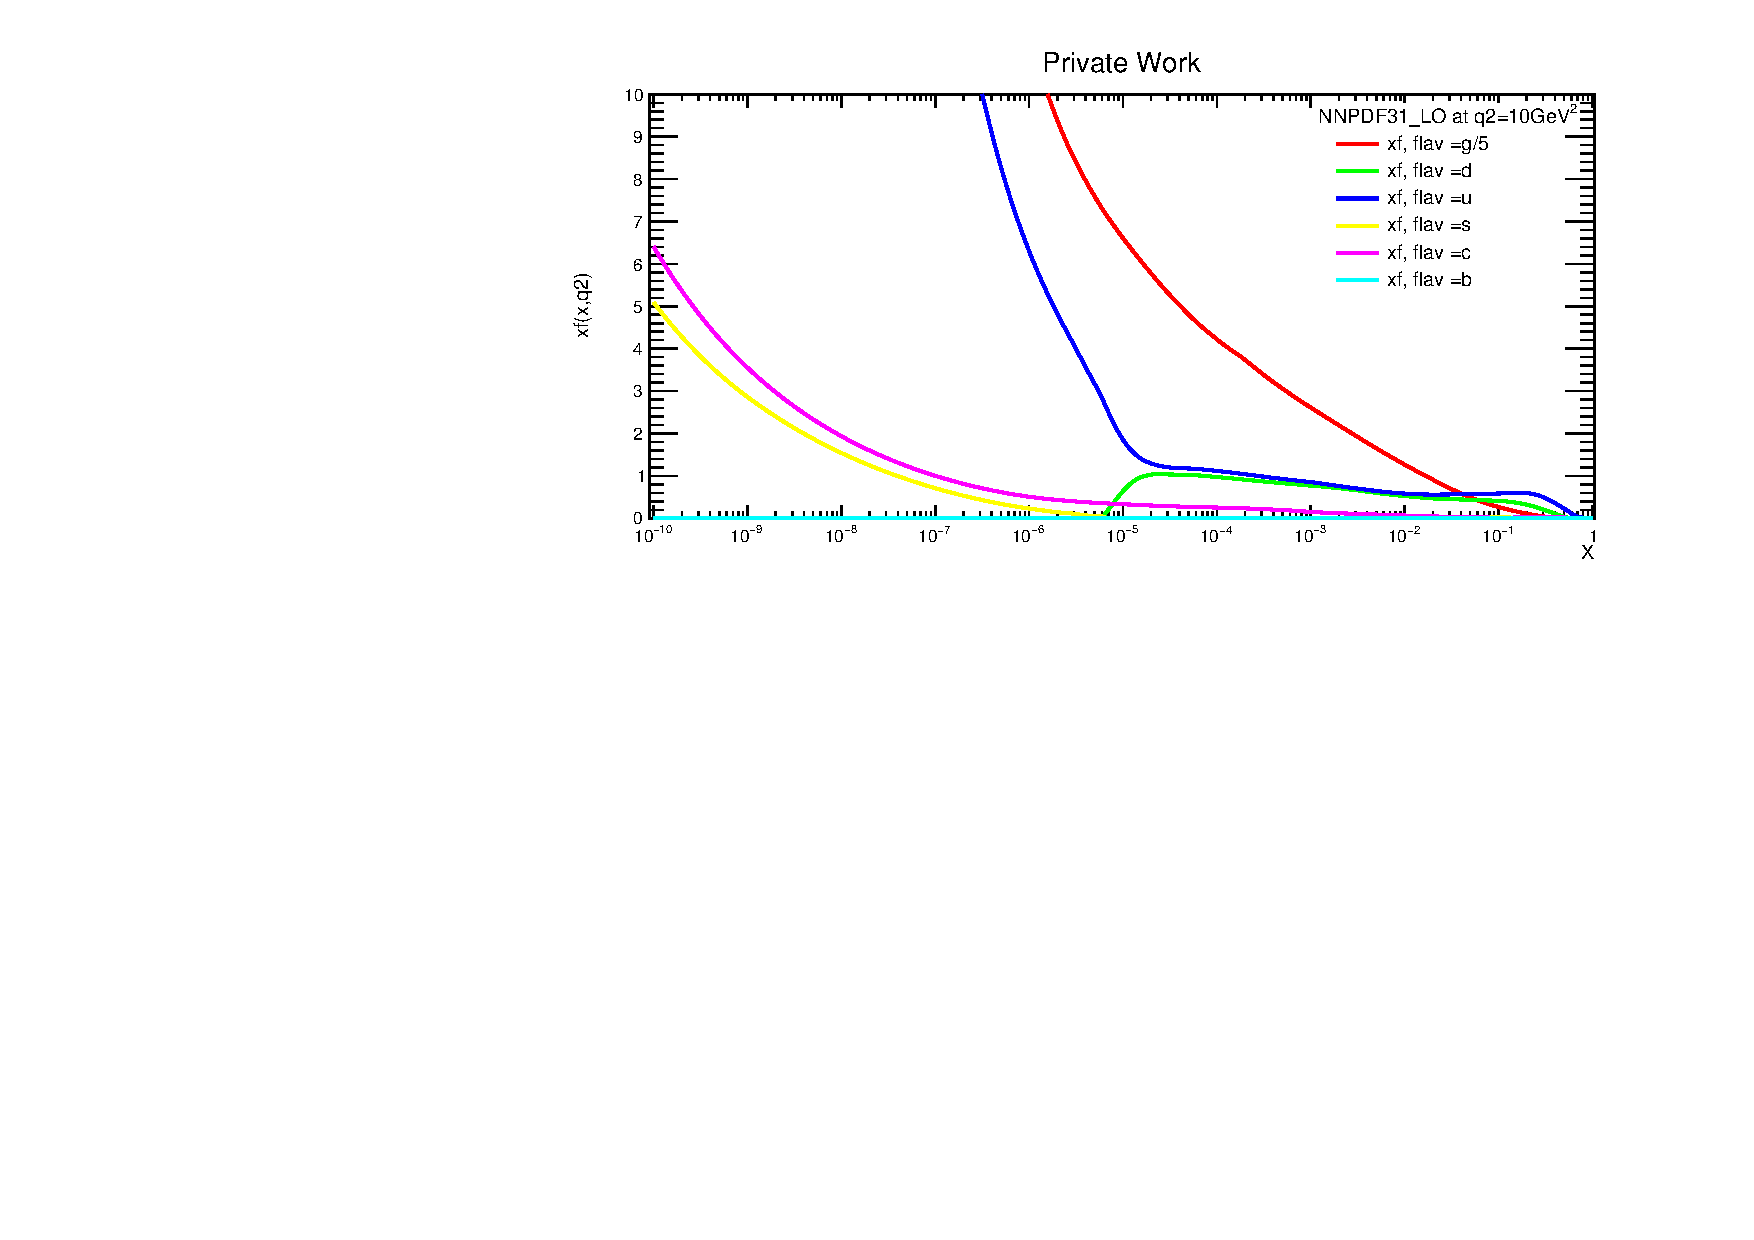
\includegraphics[height=6cm ,width=\textwidth]{chapter4/xfx10gev_lo.pdf}
\vspace*{-8mm}
\caption{}
\end{subfigure}
\begin{subfigure}{0.49\textwidth}
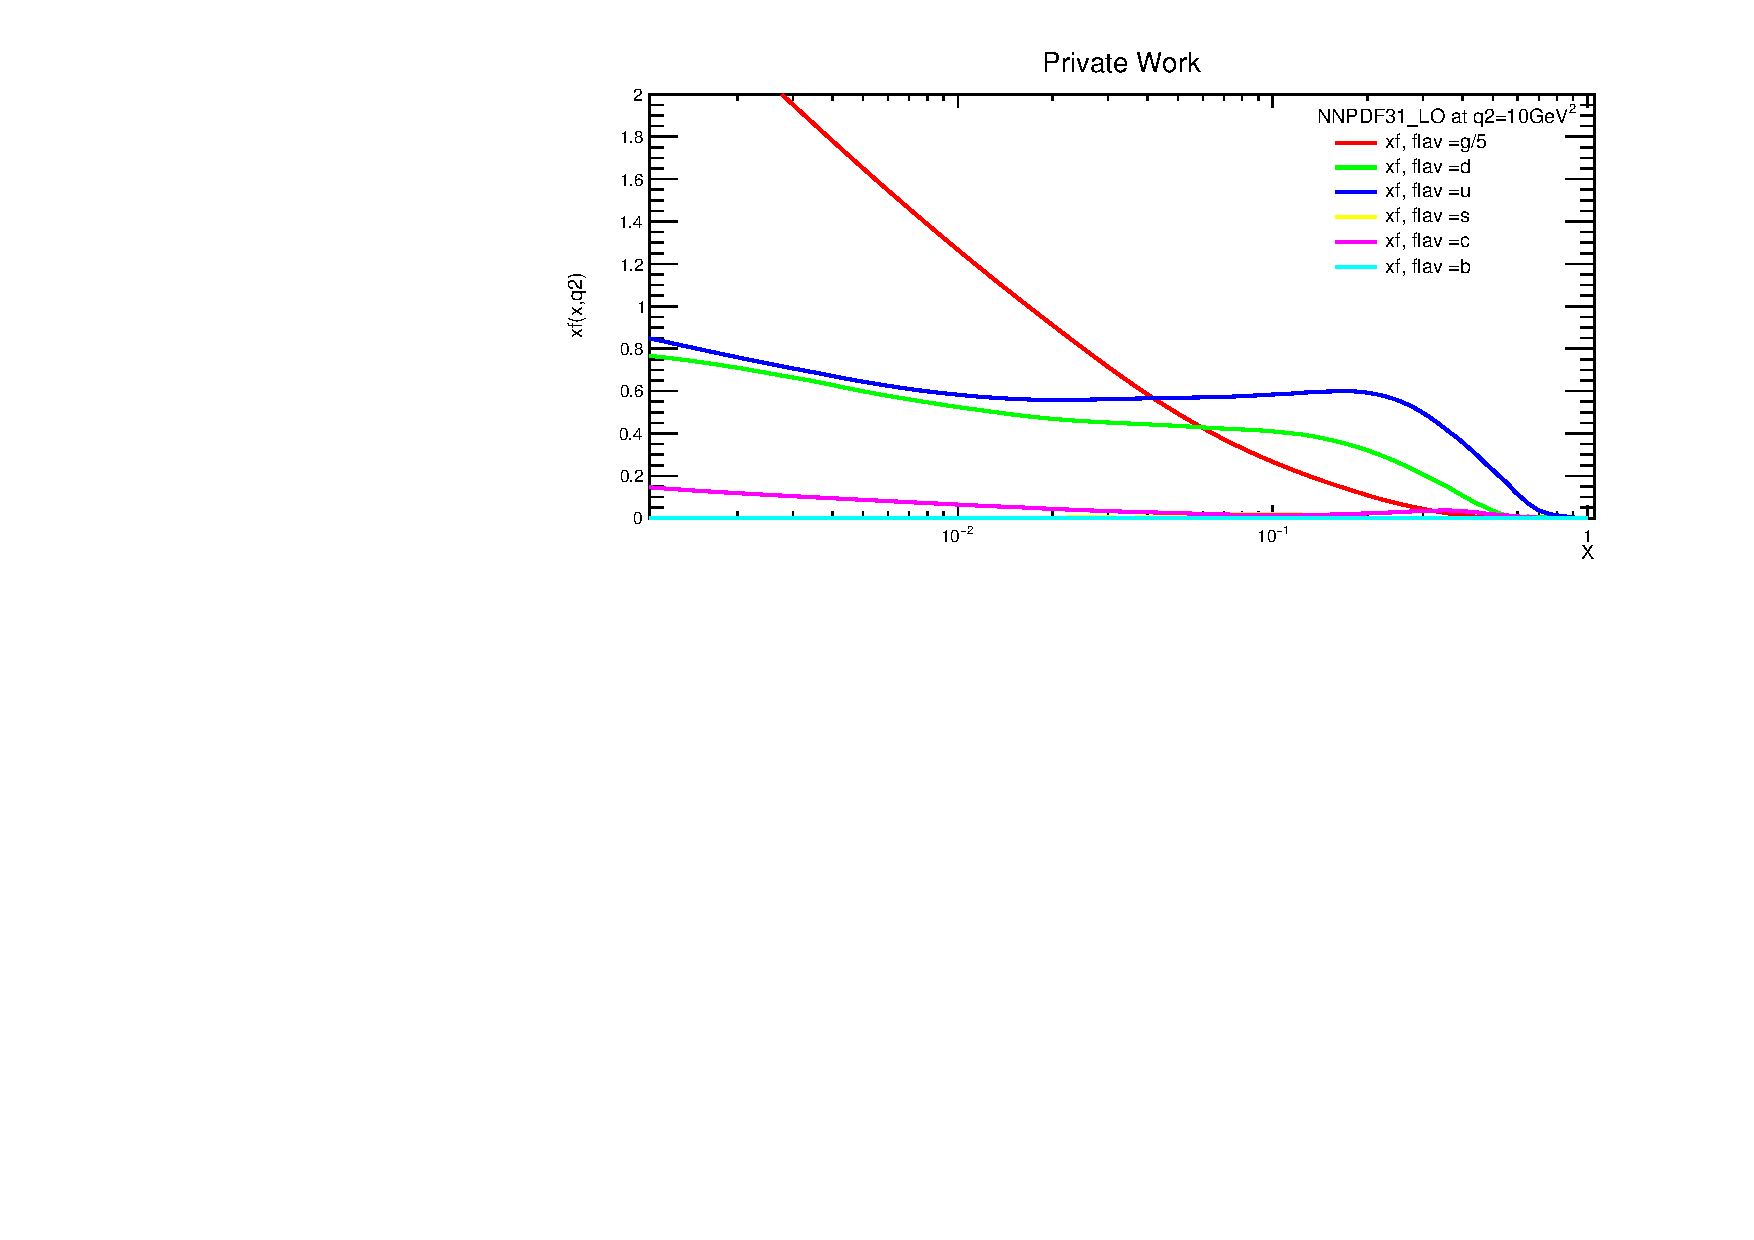
\includegraphics[height=6cm, width=\textwidth]{chapter4/xfx10gev_lo1.pdf}
\vspace*{-8mm}
\caption{}
\end{subfigure}
\begin{subfigure}{0.49\textwidth}
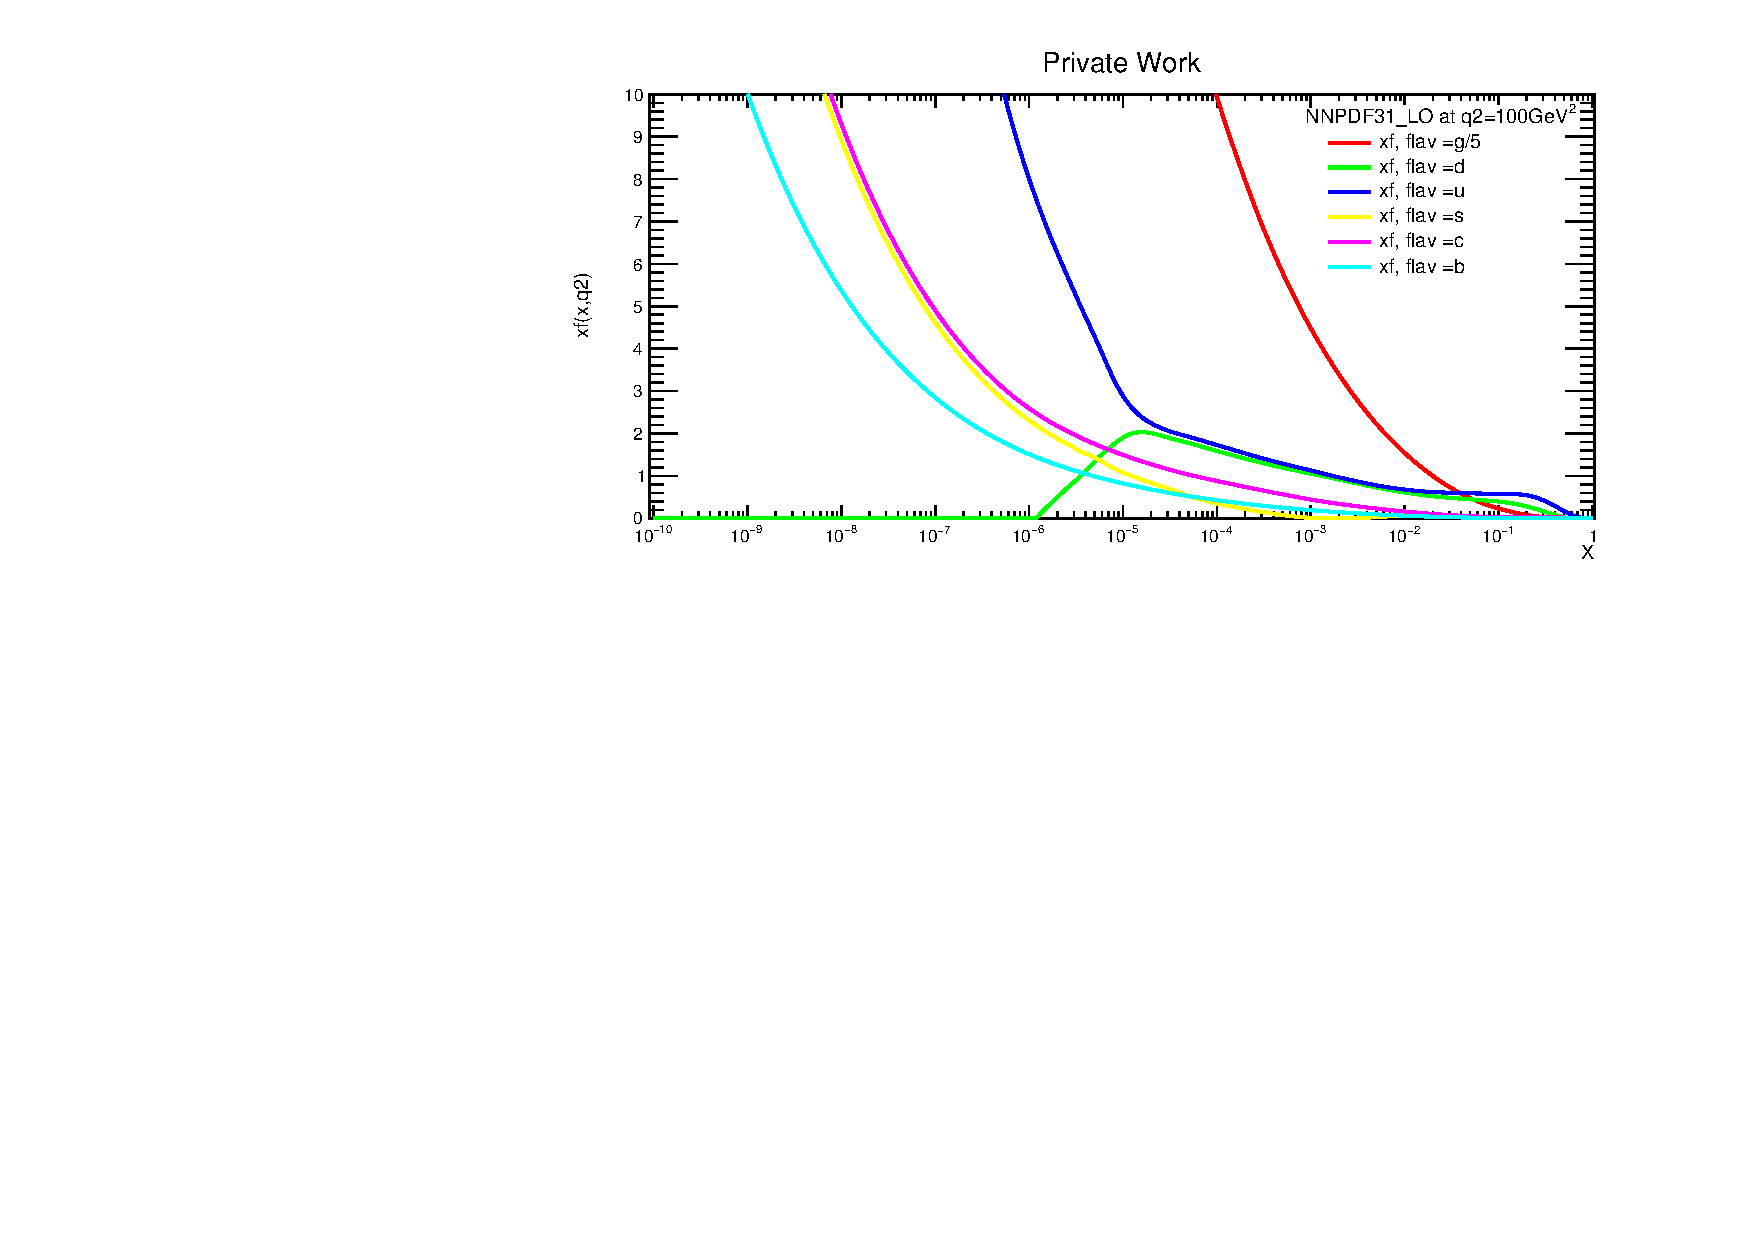
\includegraphics[height=6cm, width=\textwidth]{chapter4/xfx100gev_lo.pdf}
\vspace*{-8mm}
\caption{}
\end{subfigure}
\begin{subfigure}{0.49\textwidth}
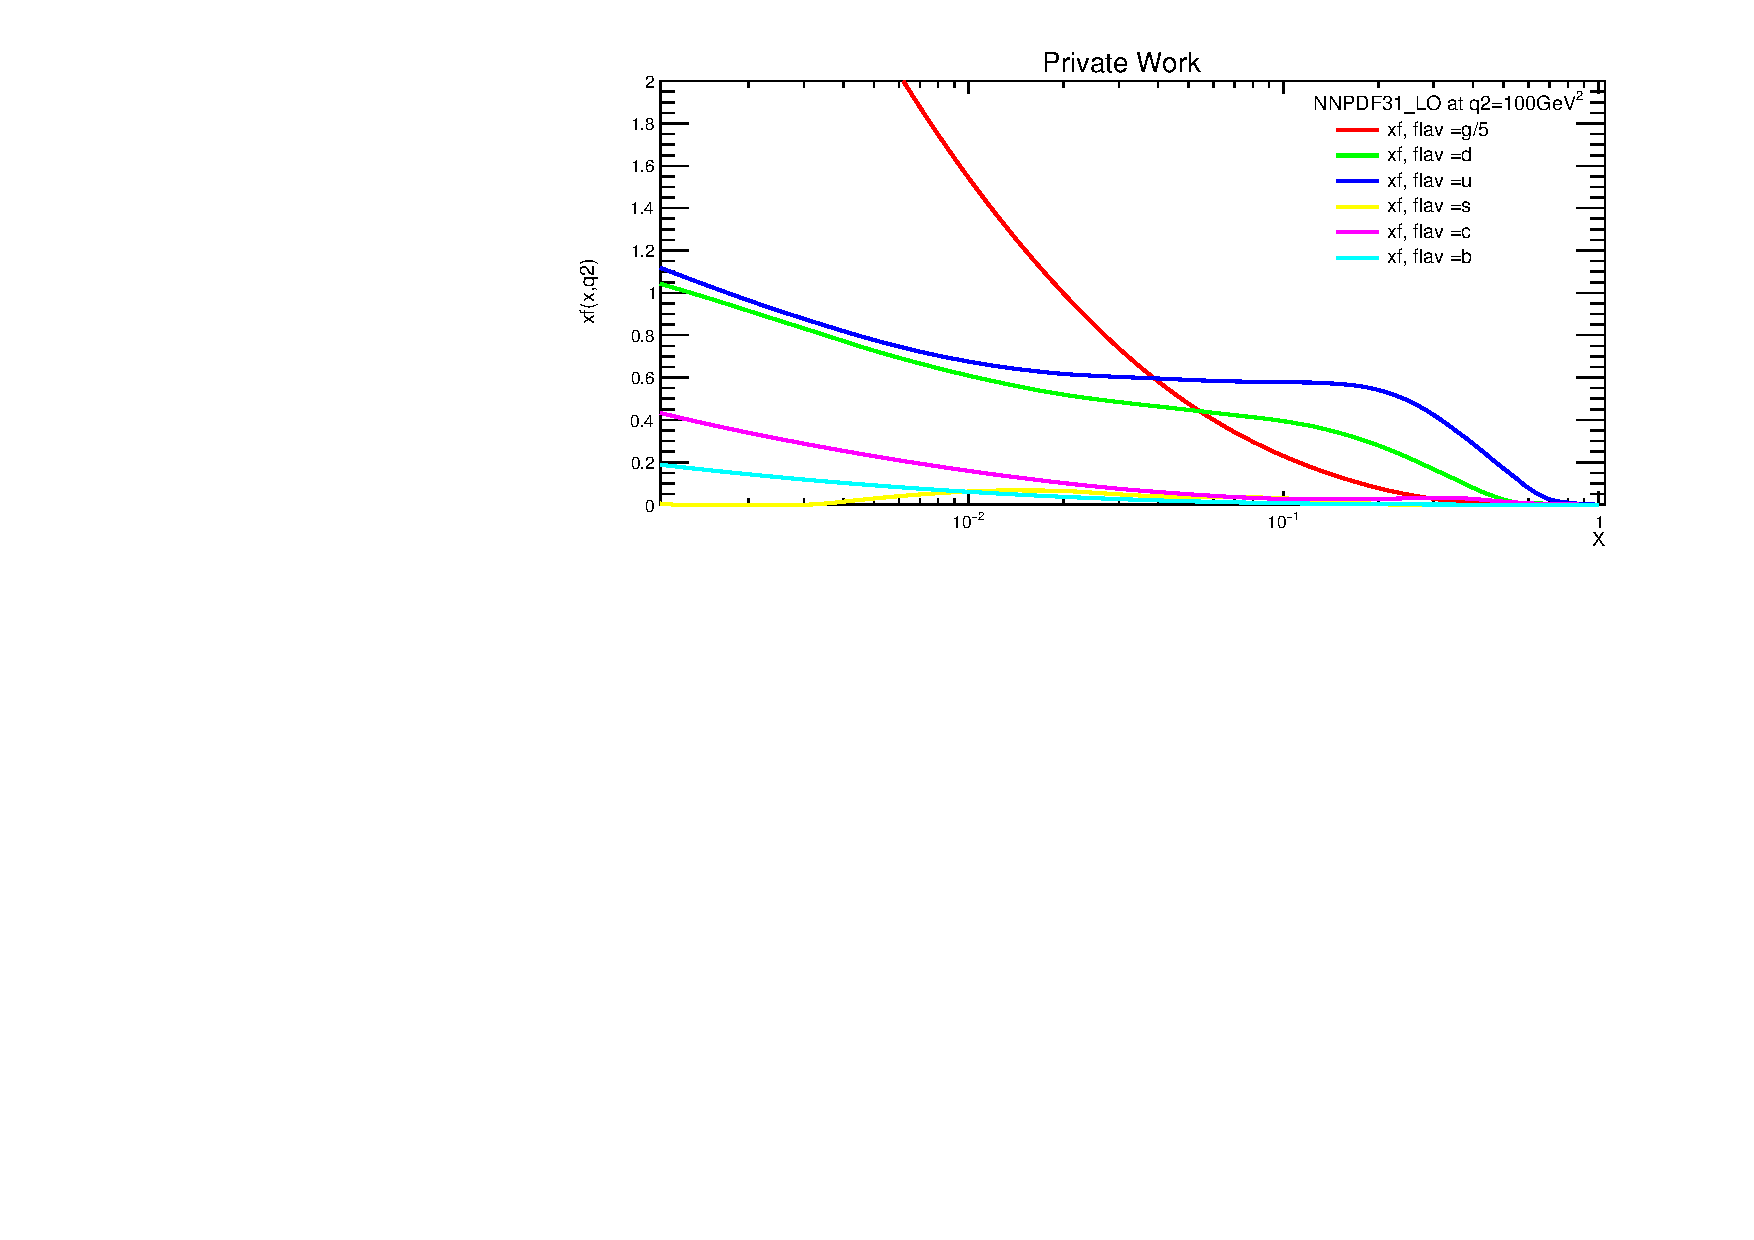
\includegraphics[height=6cm, width=\textwidth]{chapter4/xfx100gev_lo1.pdf}
\vspace*{-8mm}
\caption{}
\end{subfigure}
\begin{subfigure}{0.49\textwidth}
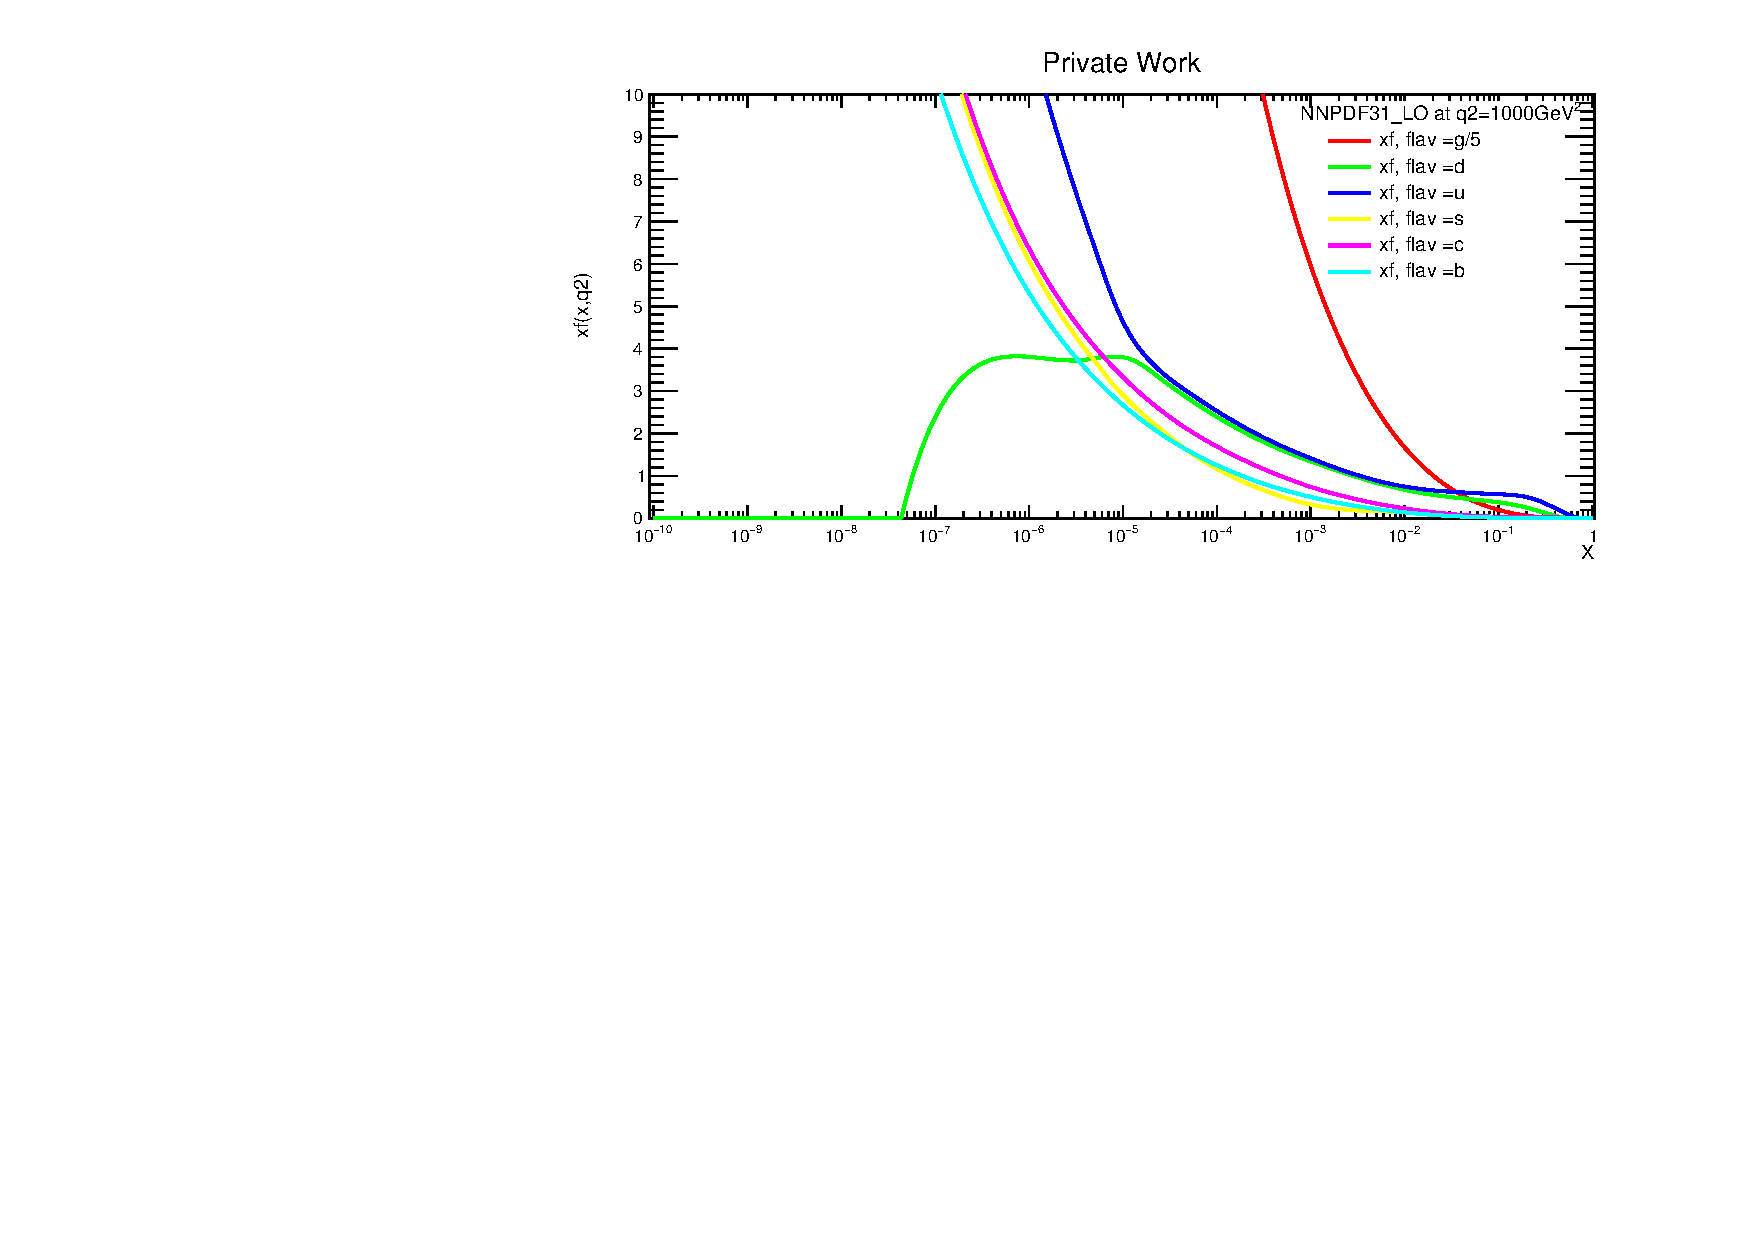
\includegraphics[height=6cm, width=\textwidth]{chapter4/xfx1000gev_lo.pdf}
\vspace*{-8mm}
\caption{}
\end{subfigure}
\begin{subfigure}{0.49\textwidth}
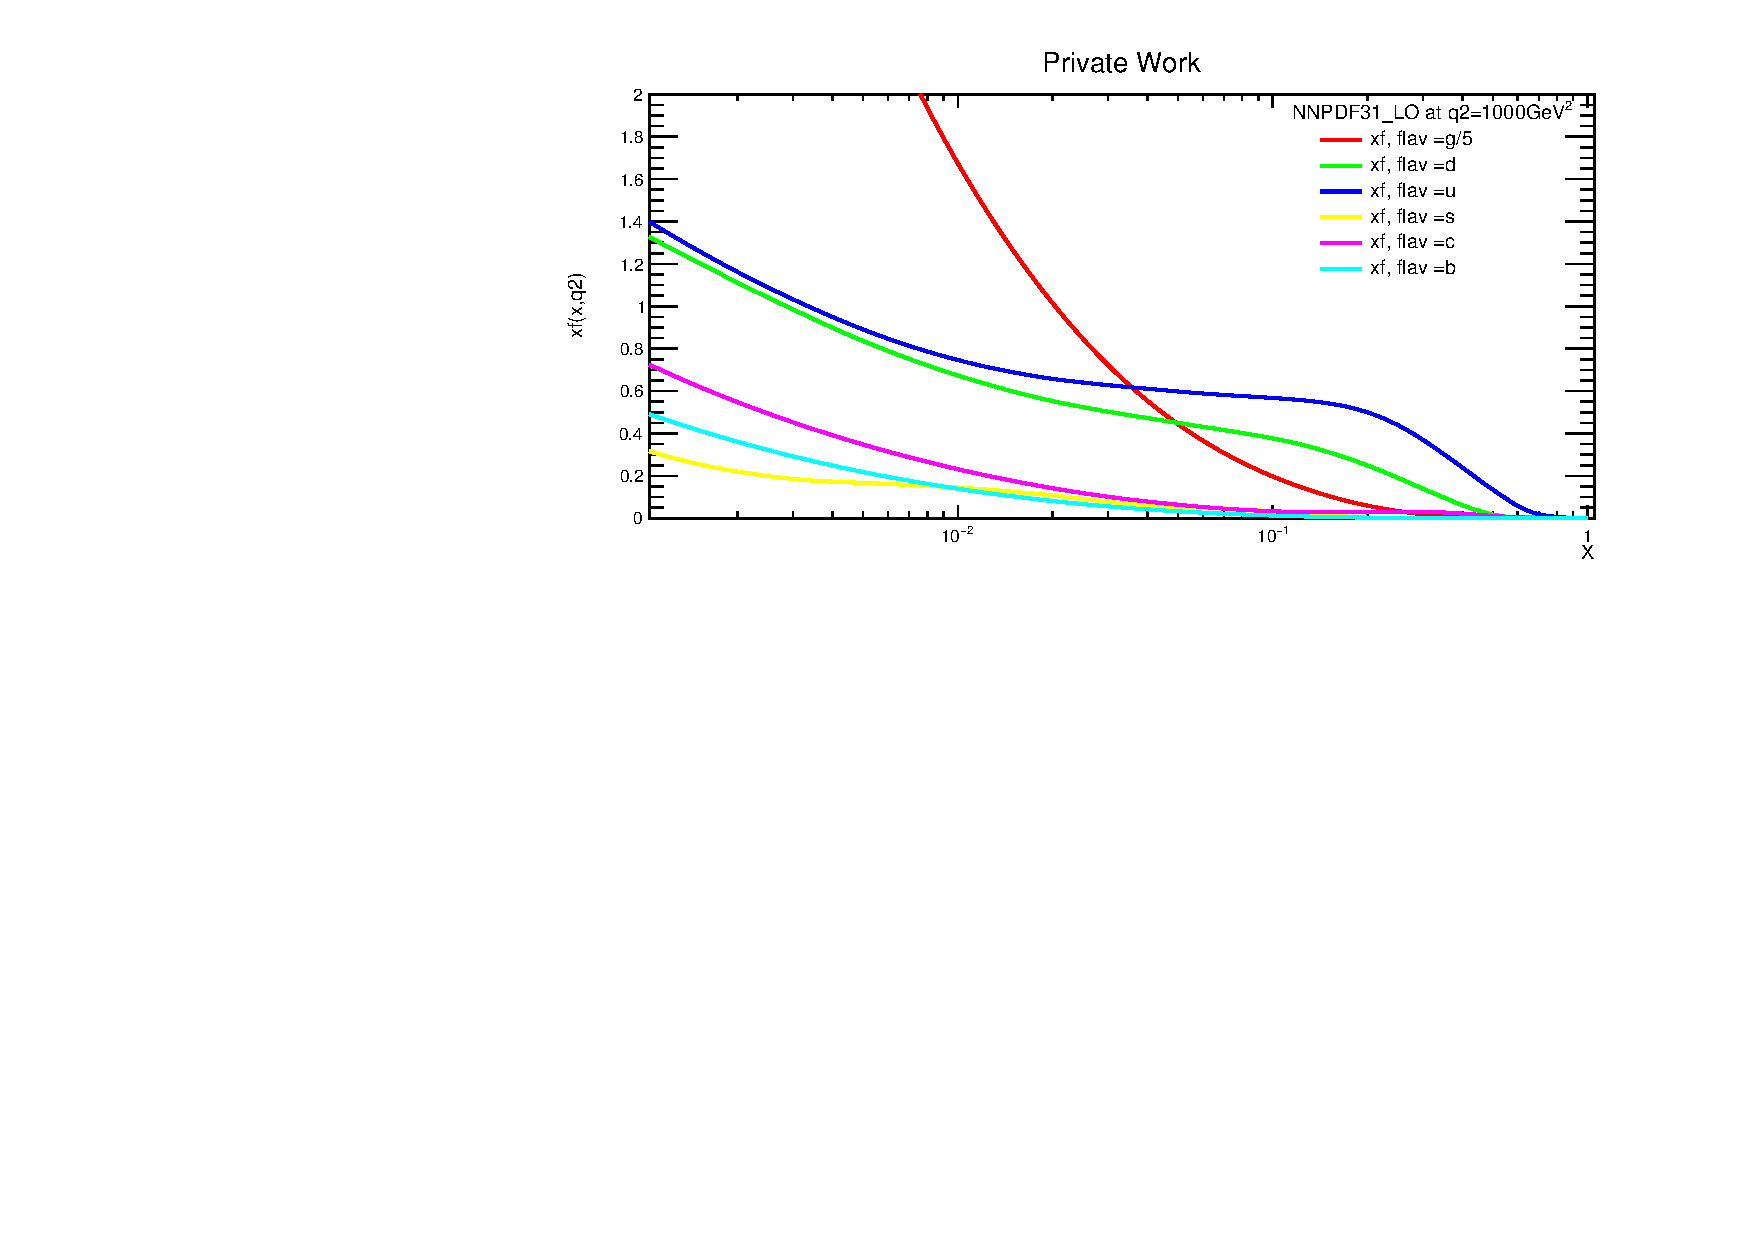
\includegraphics[height=6cm, width=\textwidth]{chapter4/xfx1000gev_lo1.pdf}
\vspace*{-8mm}
\caption{}
\end{subfigure}
\caption{The NNPDF3.1-LO PDFs for the gluon~(g), down~(d),~up(u), strange~(s), charm~(c) and bottom~(b) quarks. (a), (b): for $Q^{2}= 10GeV^{2}$, (c), (d): for $Q^{2}=100GeV^{2}$ and (e), (f): for $Q^{2}=1000GeV^{2}$} 
\label{nnpdflo}
\end{figure}

\begin{figure}[H]
\centering
\begin{subfigure}{0.45\textwidth}
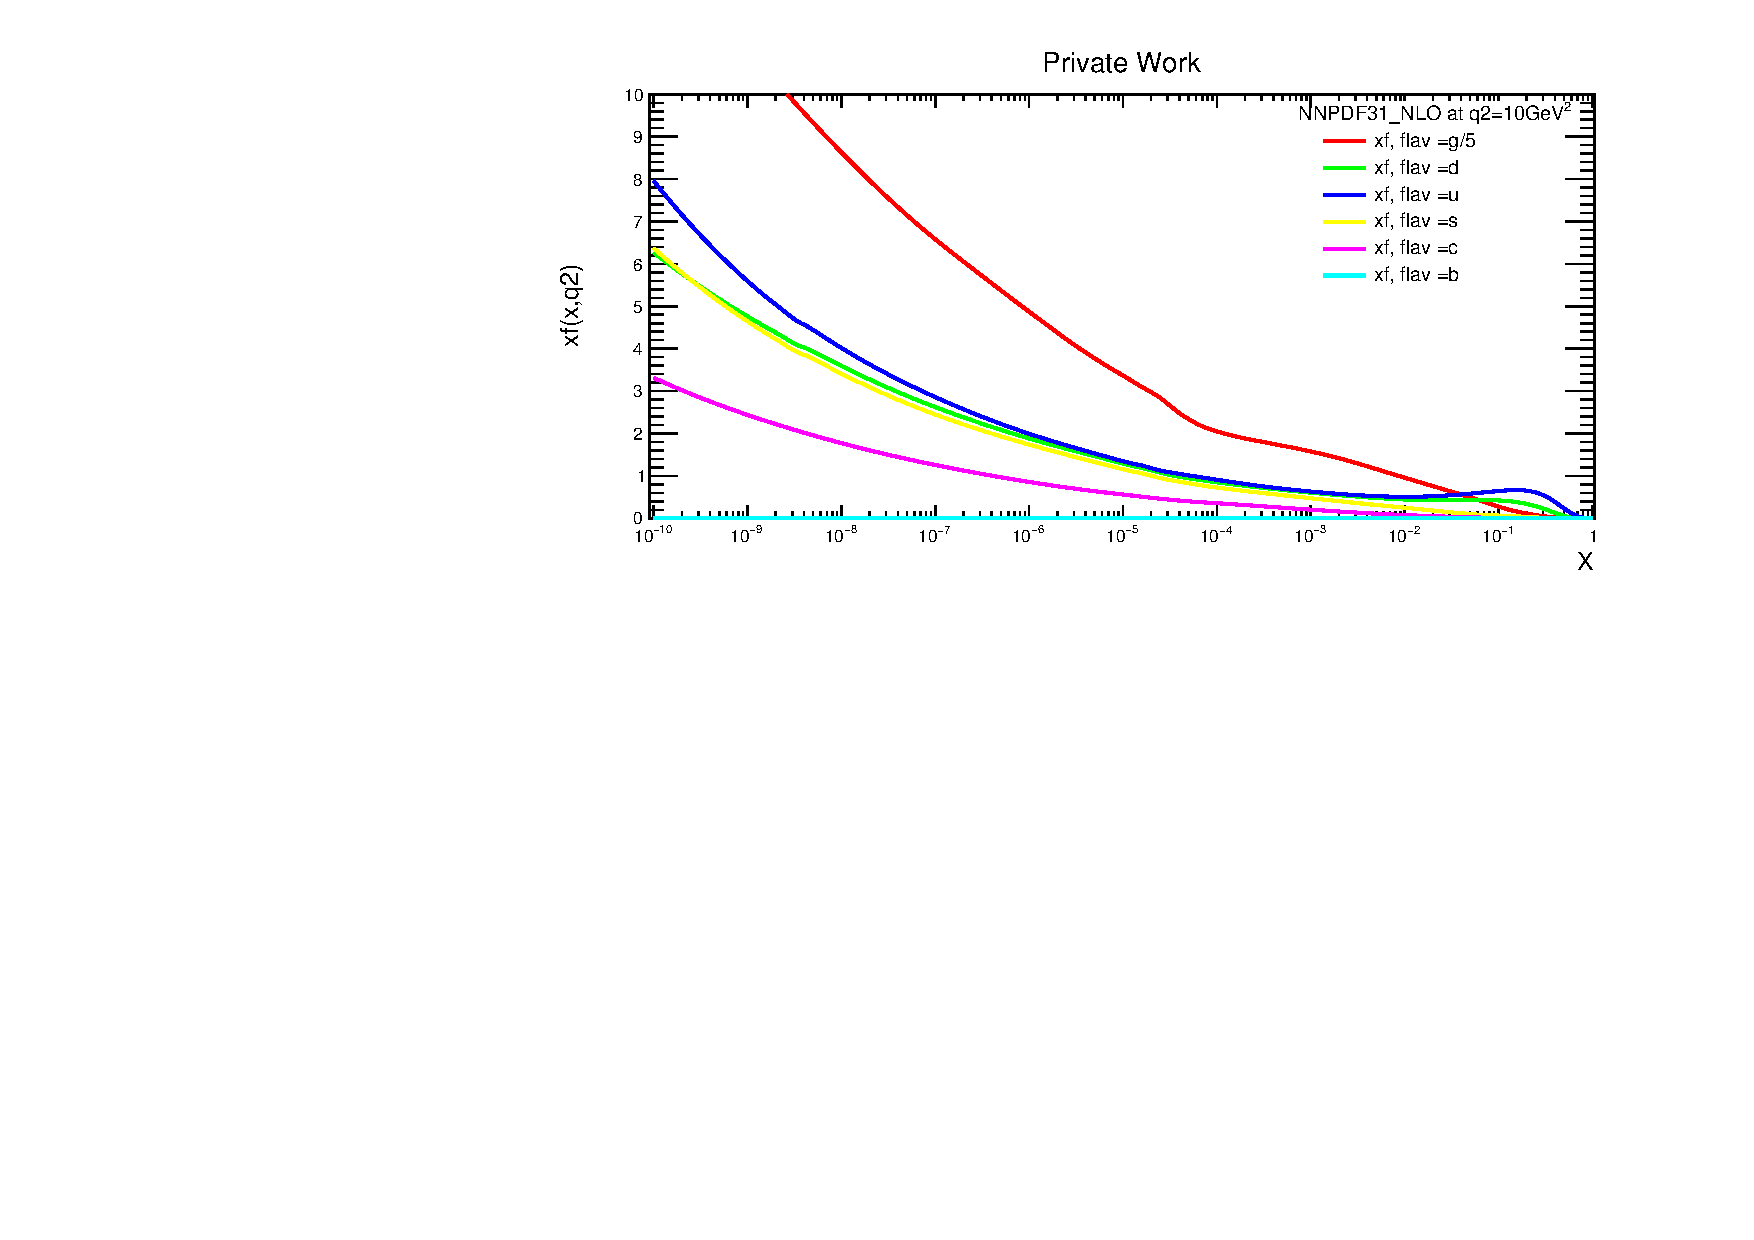
\includegraphics[height=5cm ,width=\textwidth]{chapter4/xfx10gev_nlo.pdf}
\vspace*{-8mm}
\caption{}
\end{subfigure}
\begin{subfigure}{0.45\textwidth}
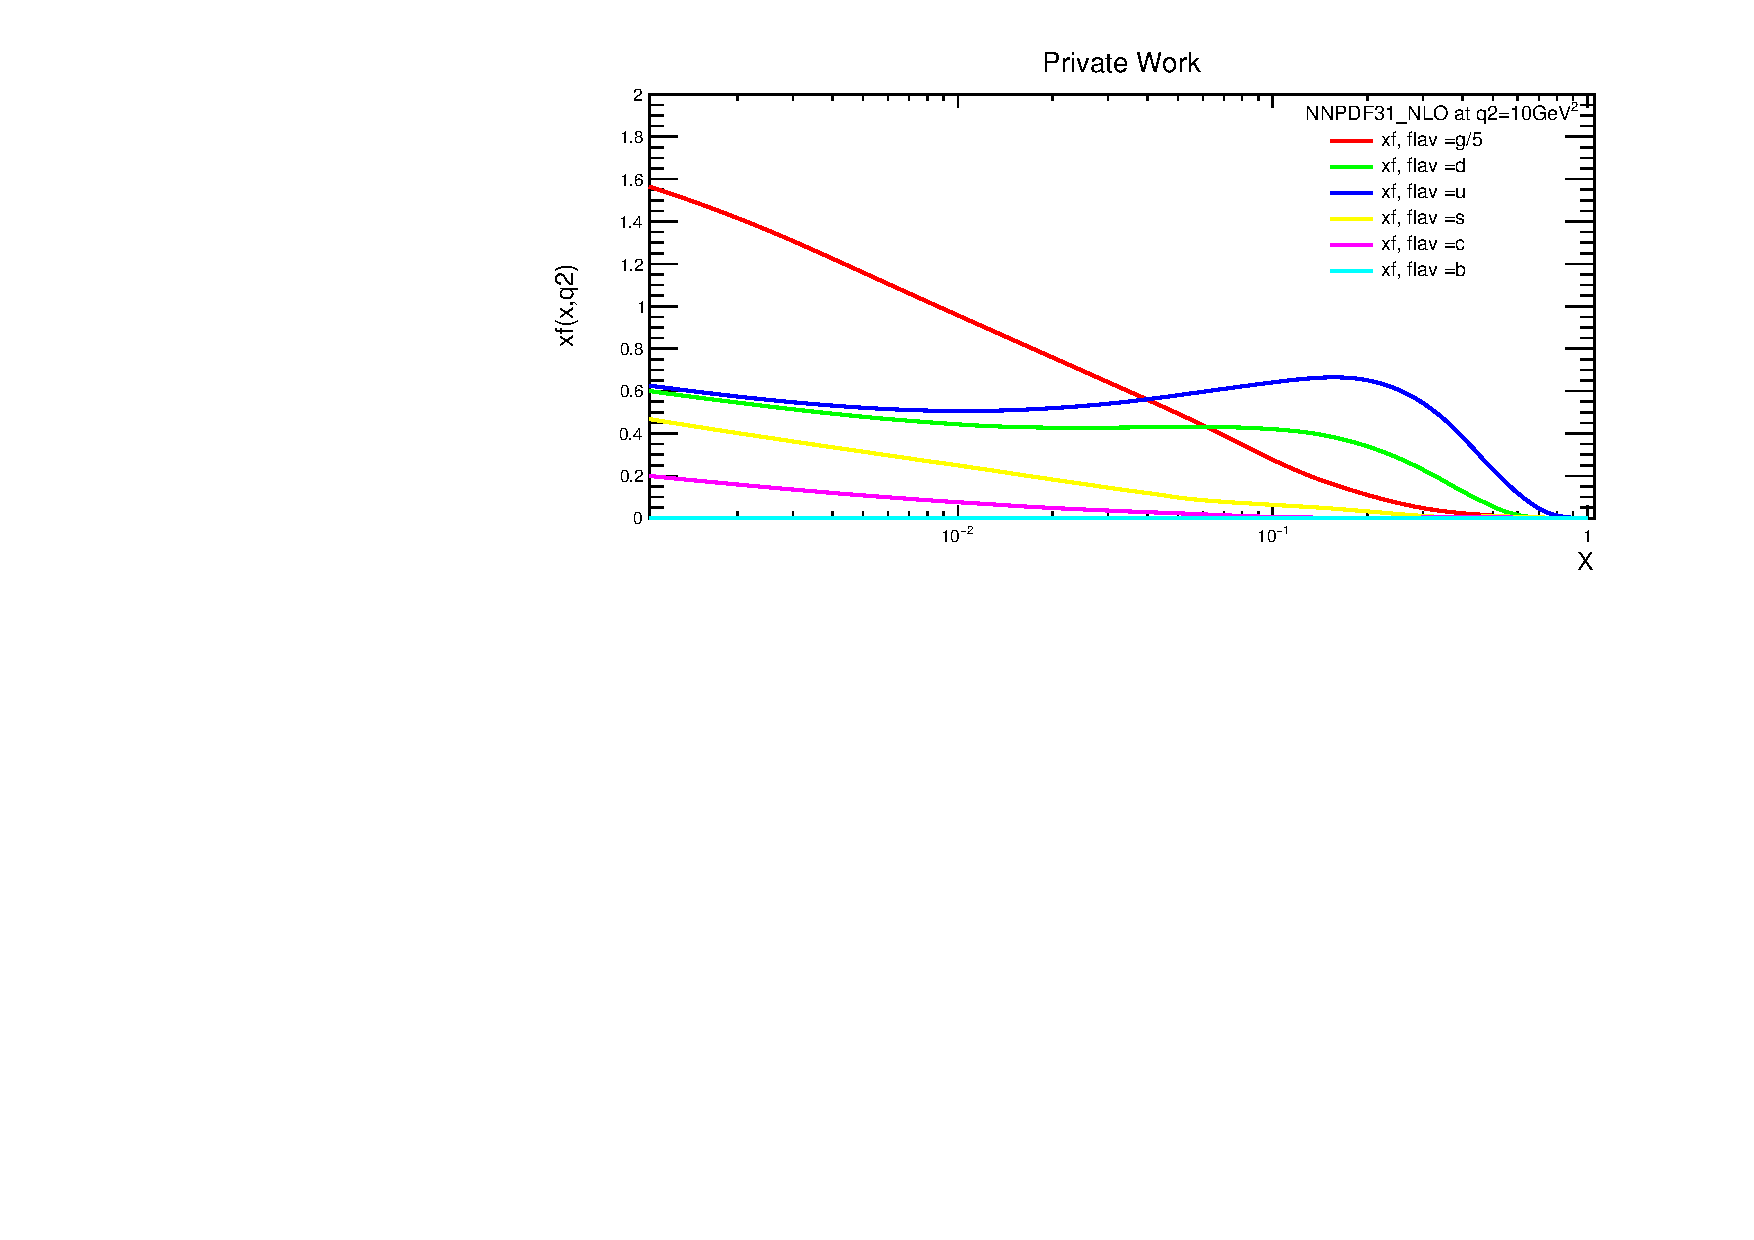
\includegraphics[height=5cm, width=\textwidth]{chapter4/xfx10gev_nlo1.pdf}
\vspace*{-8mm}
\caption{}
\end{subfigure}
\begin{subfigure}{0.45\textwidth}
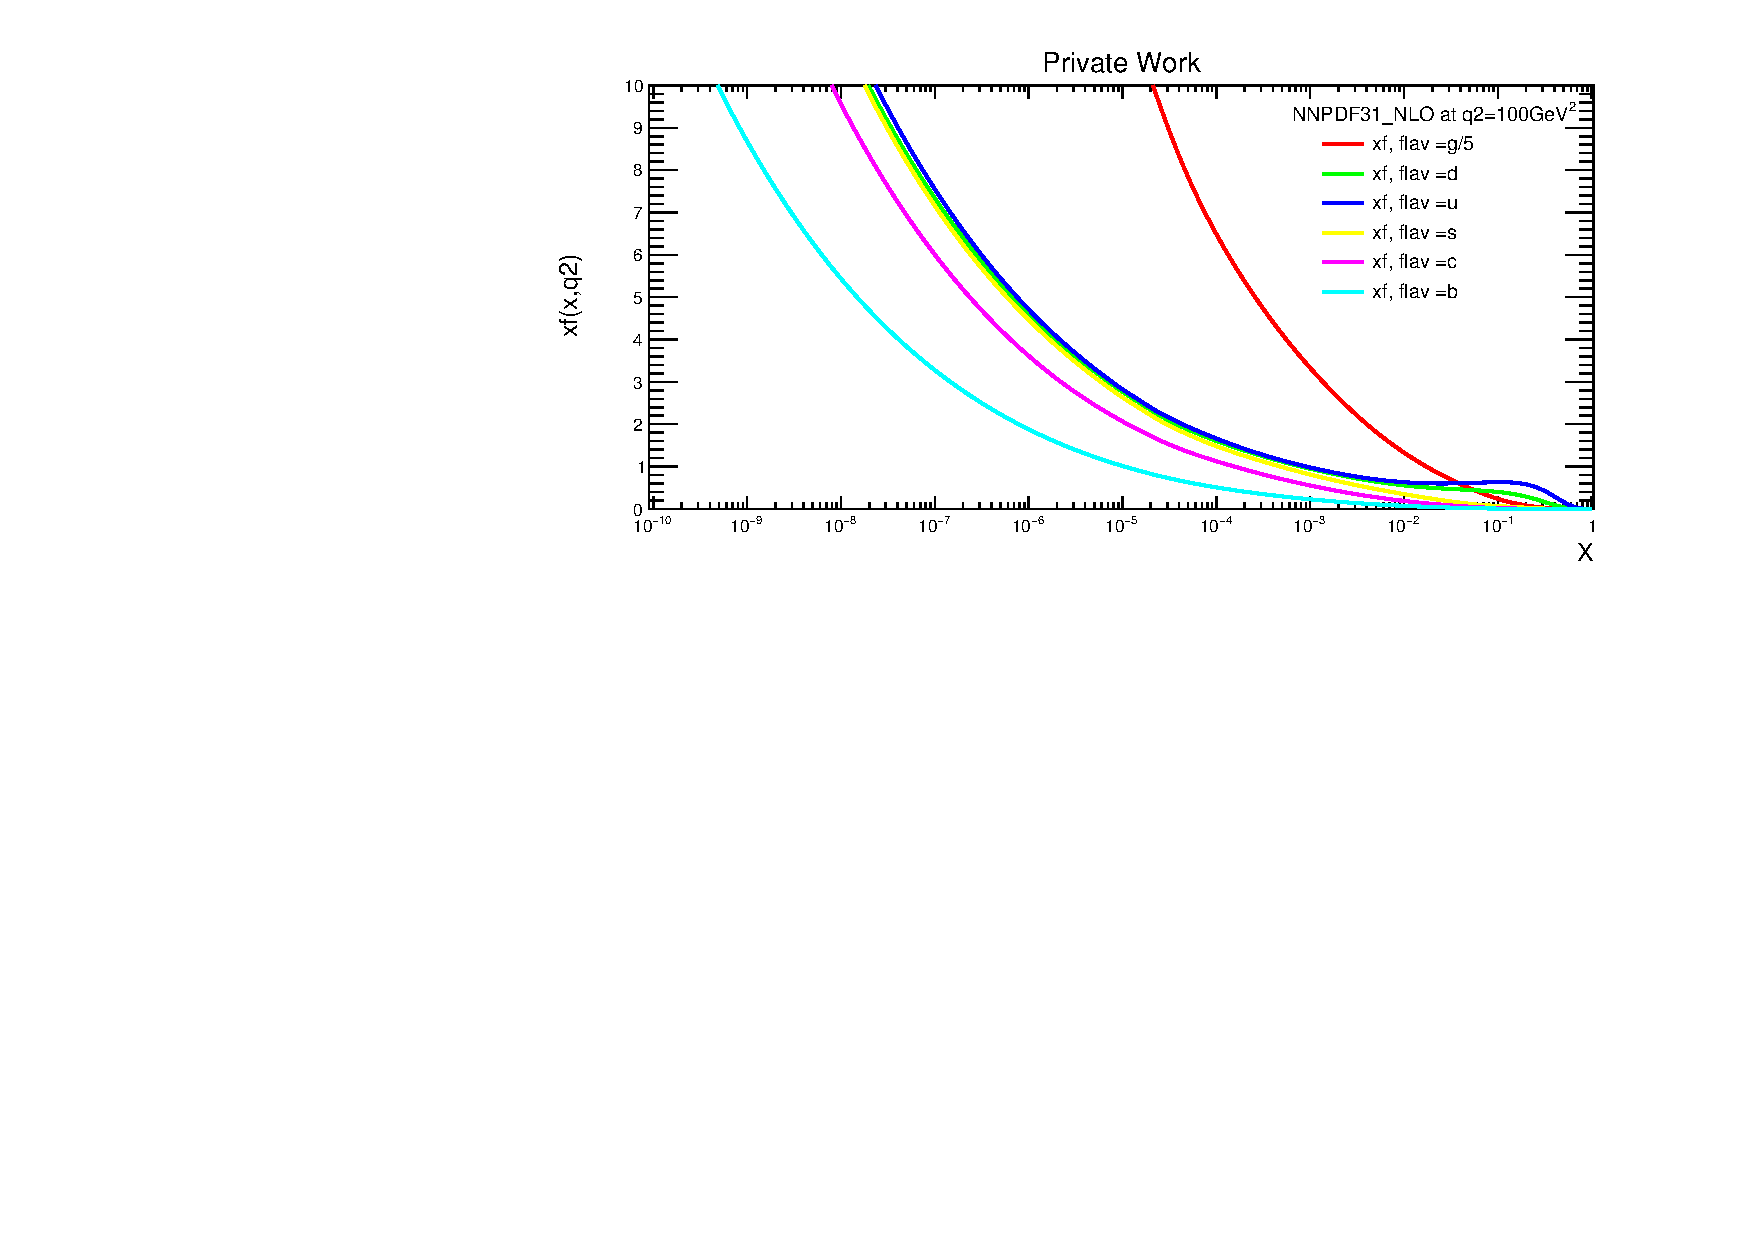
\includegraphics[height=5cm, width=\textwidth]{chapter4/xfx100gev_nlo.pdf}
\vspace*{-8mm}
\caption{}
\end{subfigure}
\begin{subfigure}{0.45\textwidth}
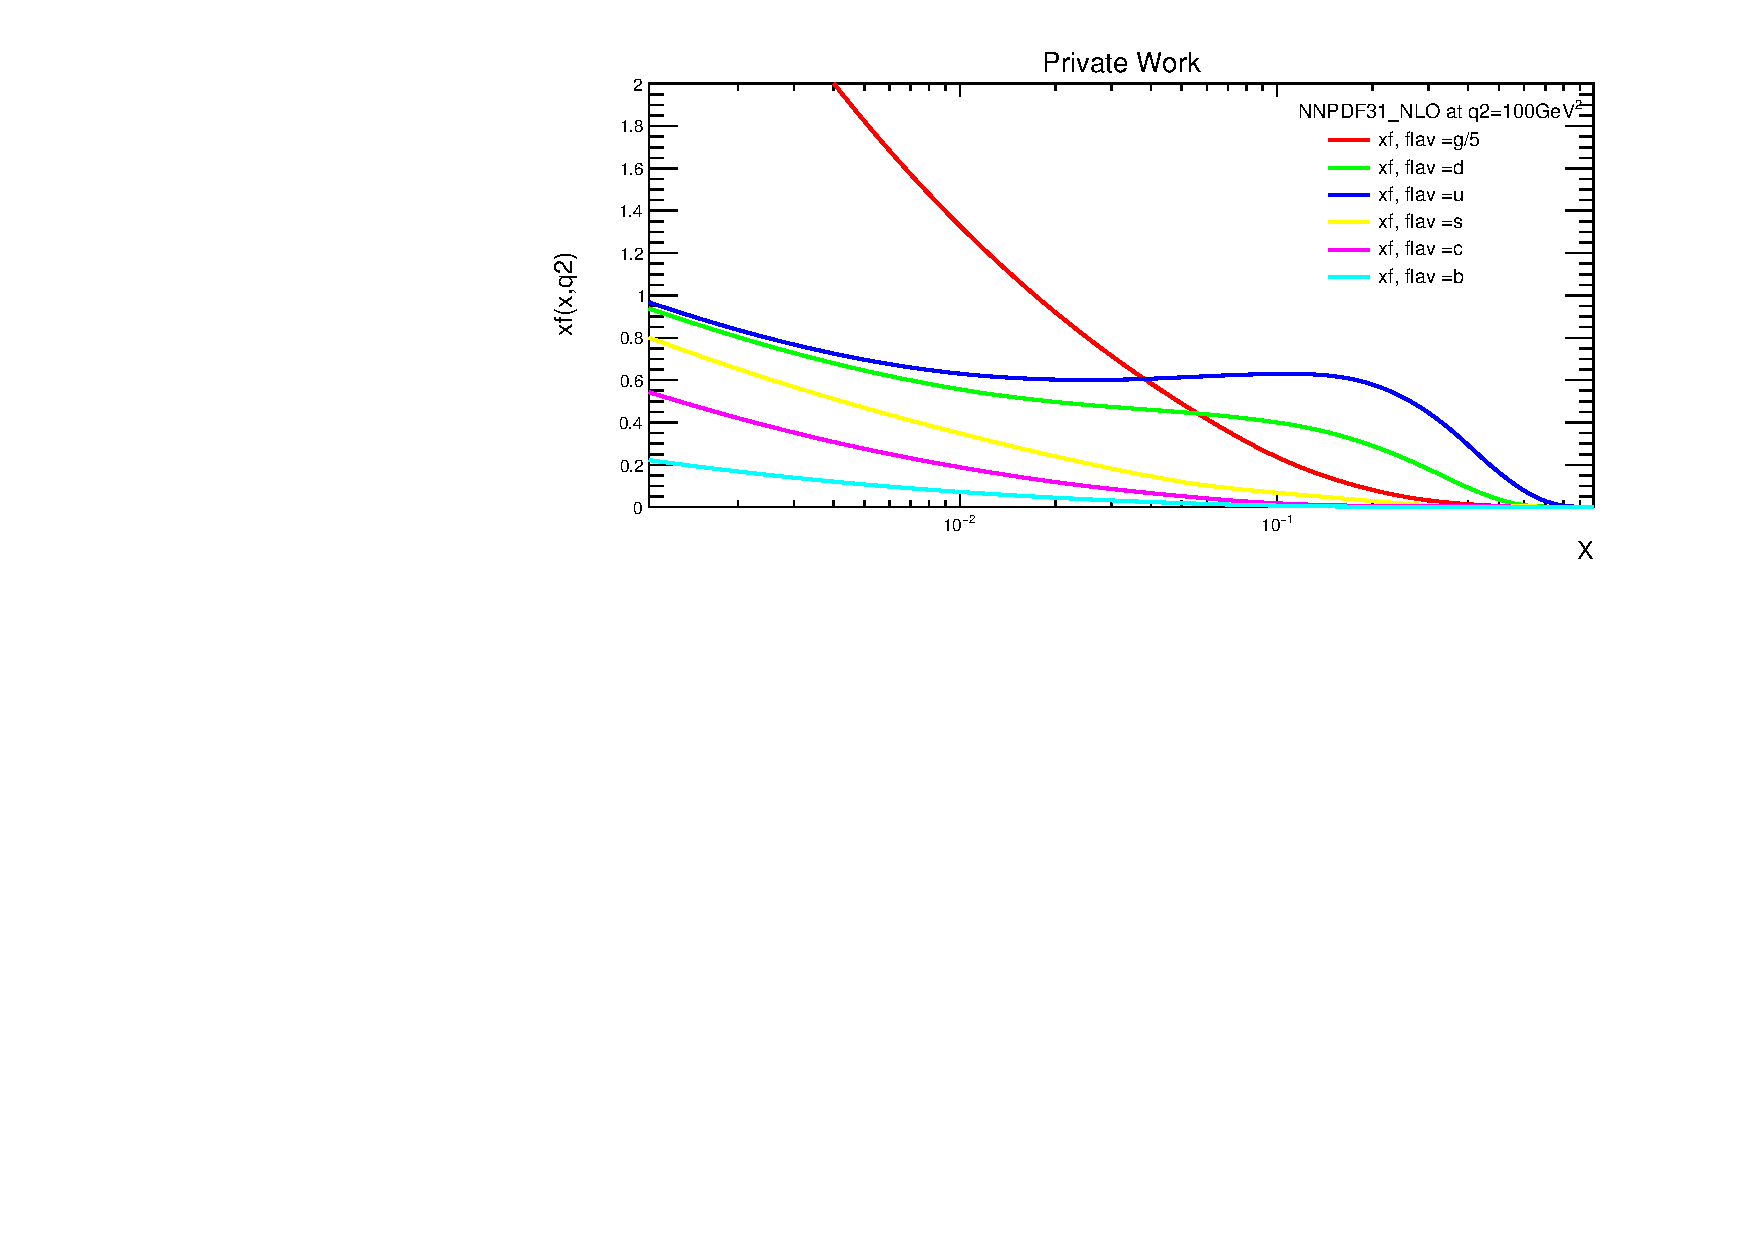
\includegraphics[height=5cm, width=\textwidth]{chapter4/xfx100gev_nlo1.pdf}
\vspace*{-8mm}
\caption{}
\end{subfigure}
\begin{subfigure}{0.45\textwidth}
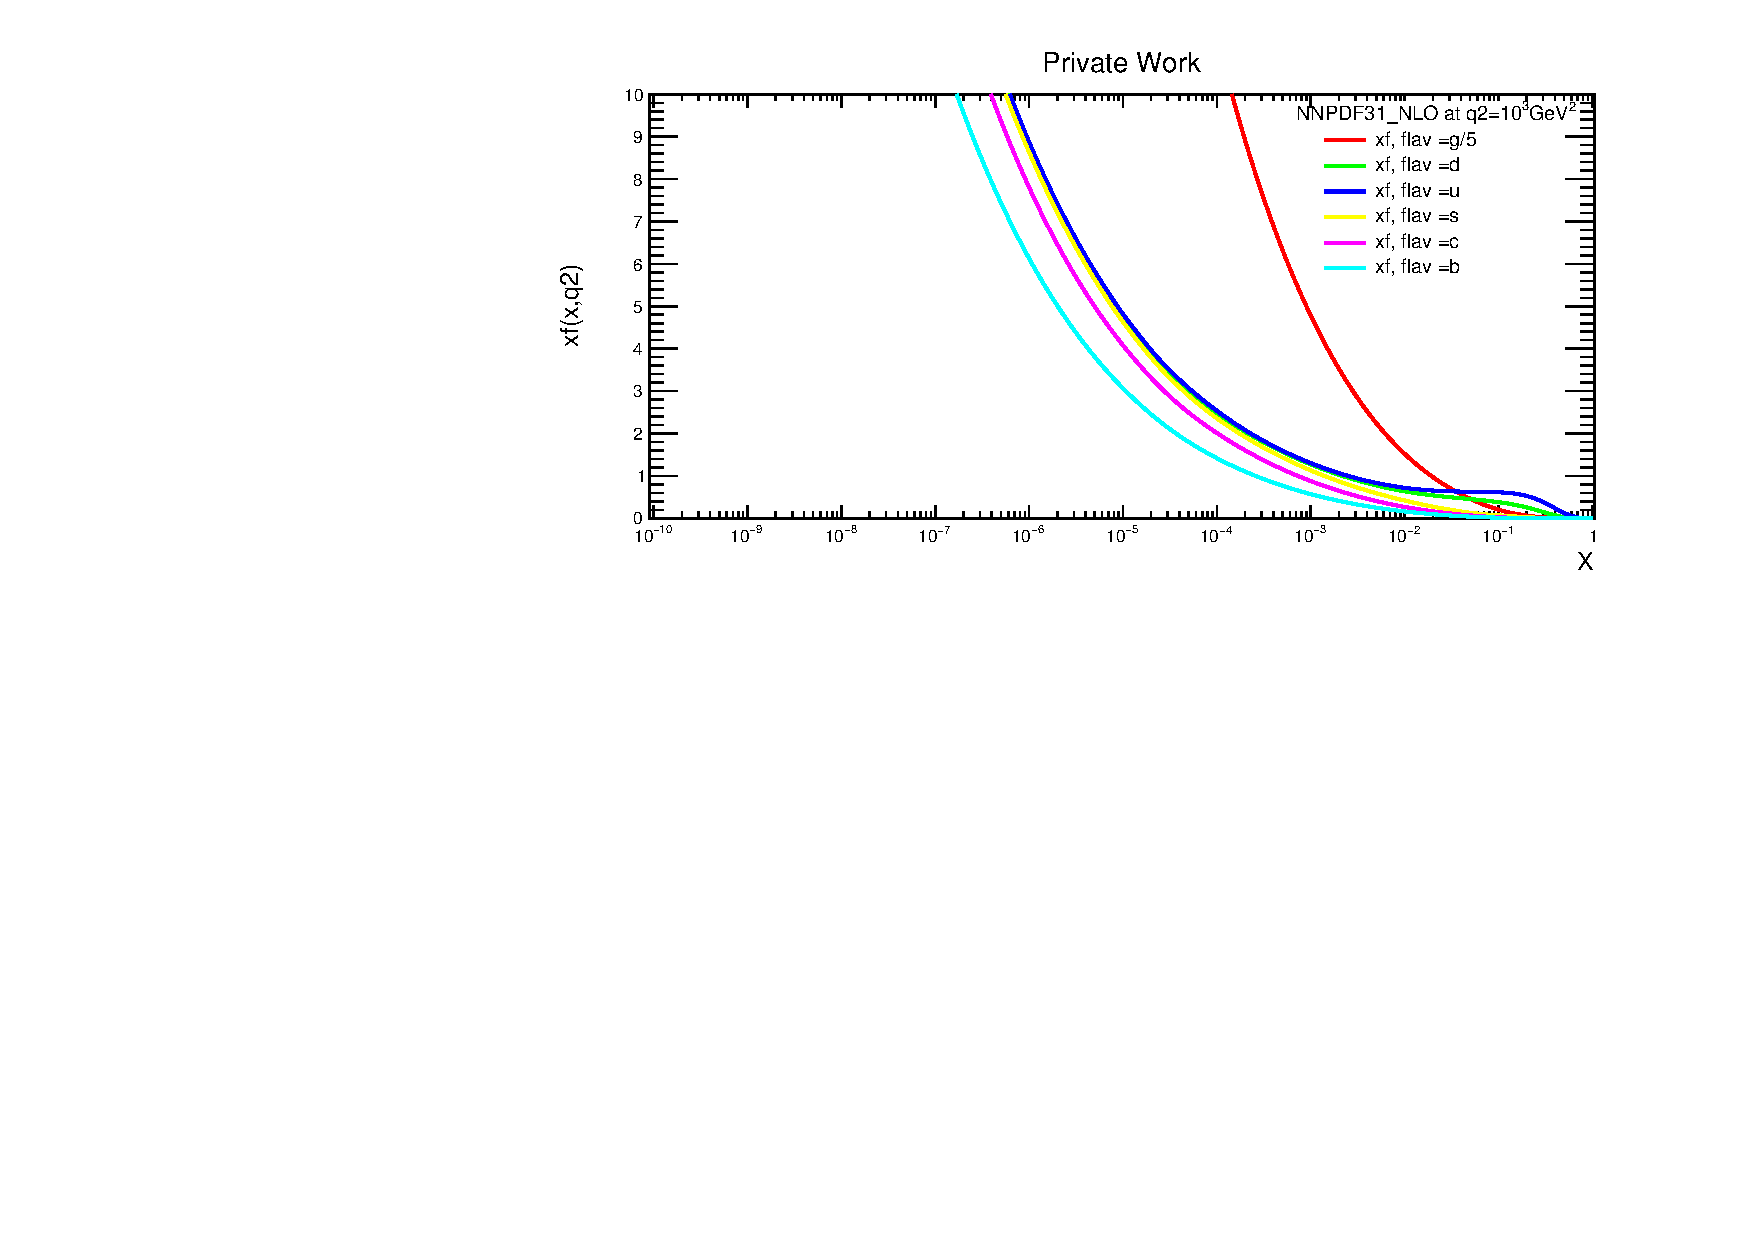
\includegraphics[height=5cm, width=\textwidth]{chapter4/xfx1000gev_nlo.pdf}
\vspace*{-8mm}
\caption{}
\end{subfigure}
\begin{subfigure}{0.45\textwidth}
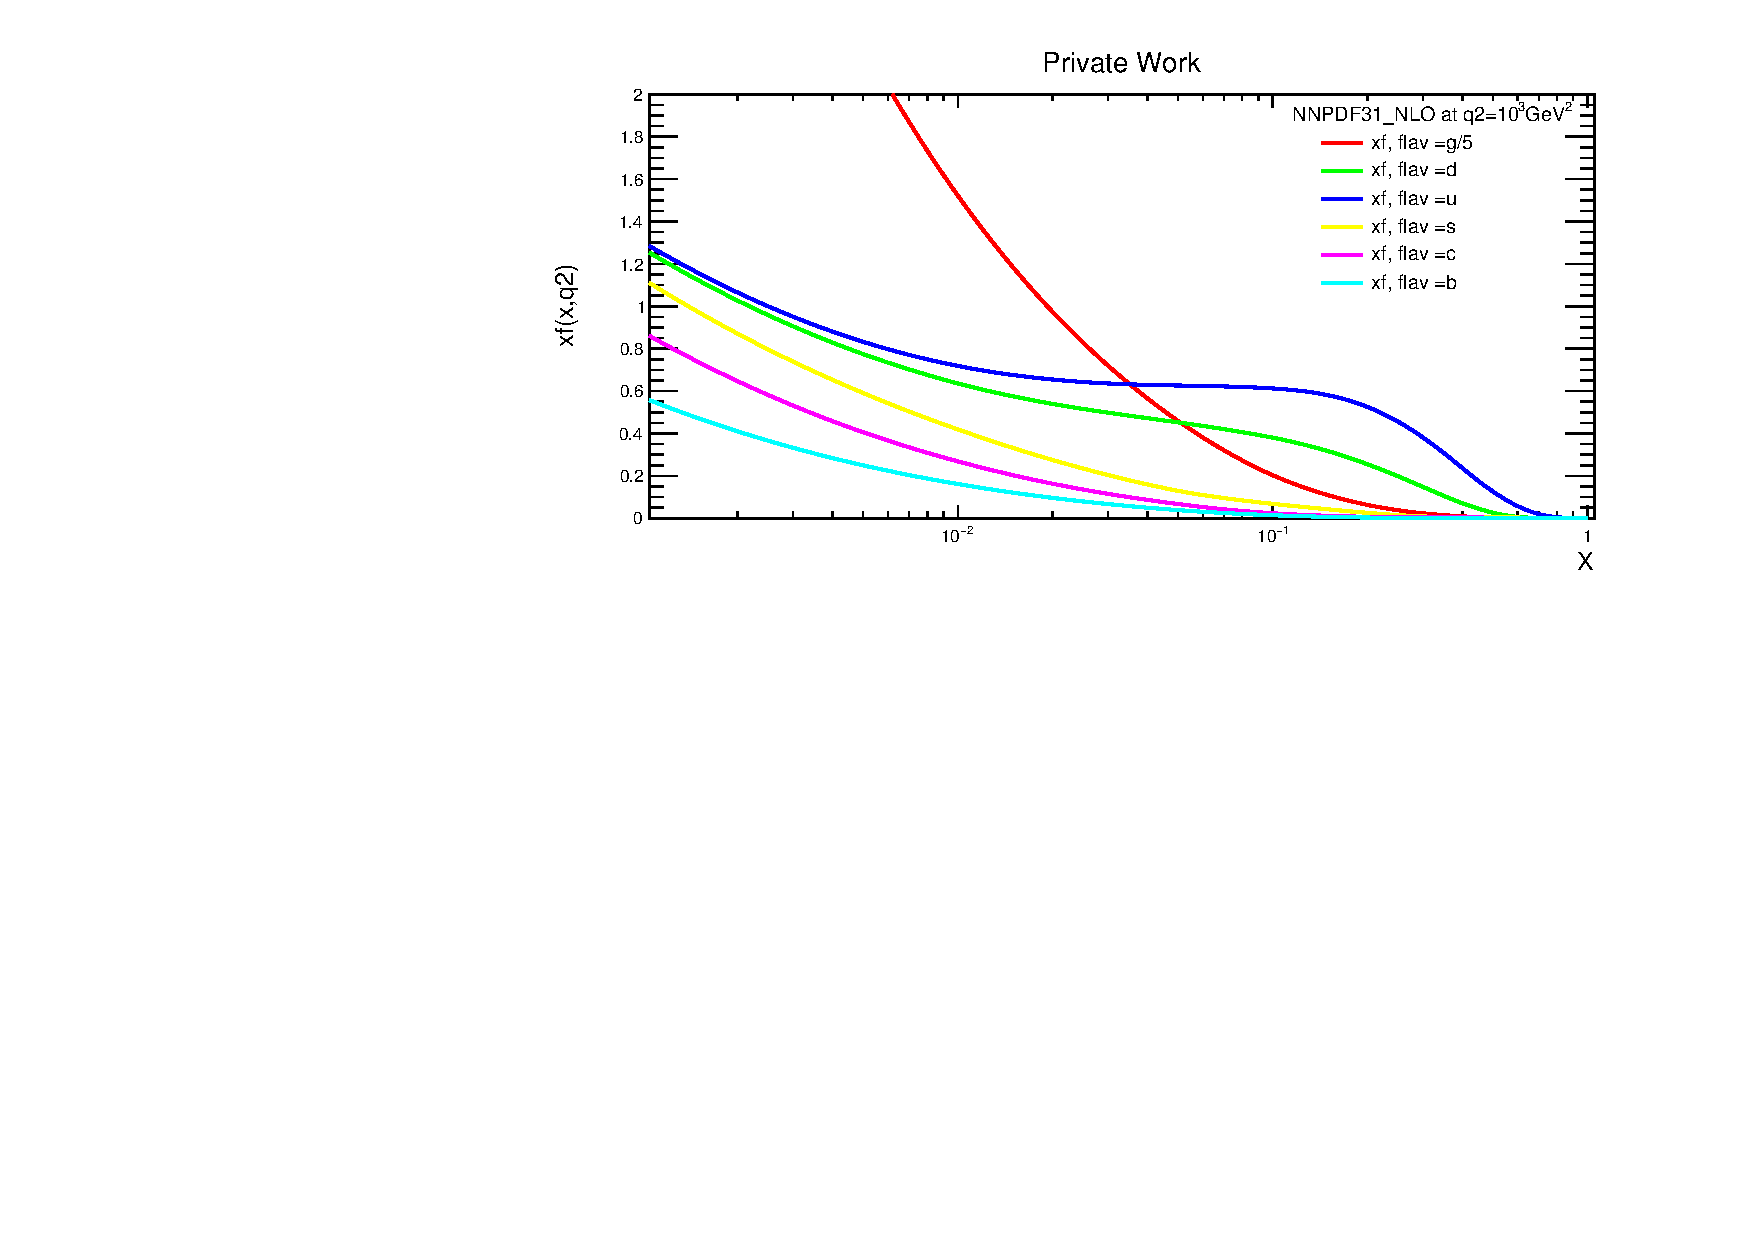
\includegraphics[height=5cm, width=\textwidth]{chapter4/xfx1000gev_nlo1.pdf}
\vspace*{-8mm}
\caption{}
\end{subfigure}
\begin{subfigure}{0.45\textwidth}
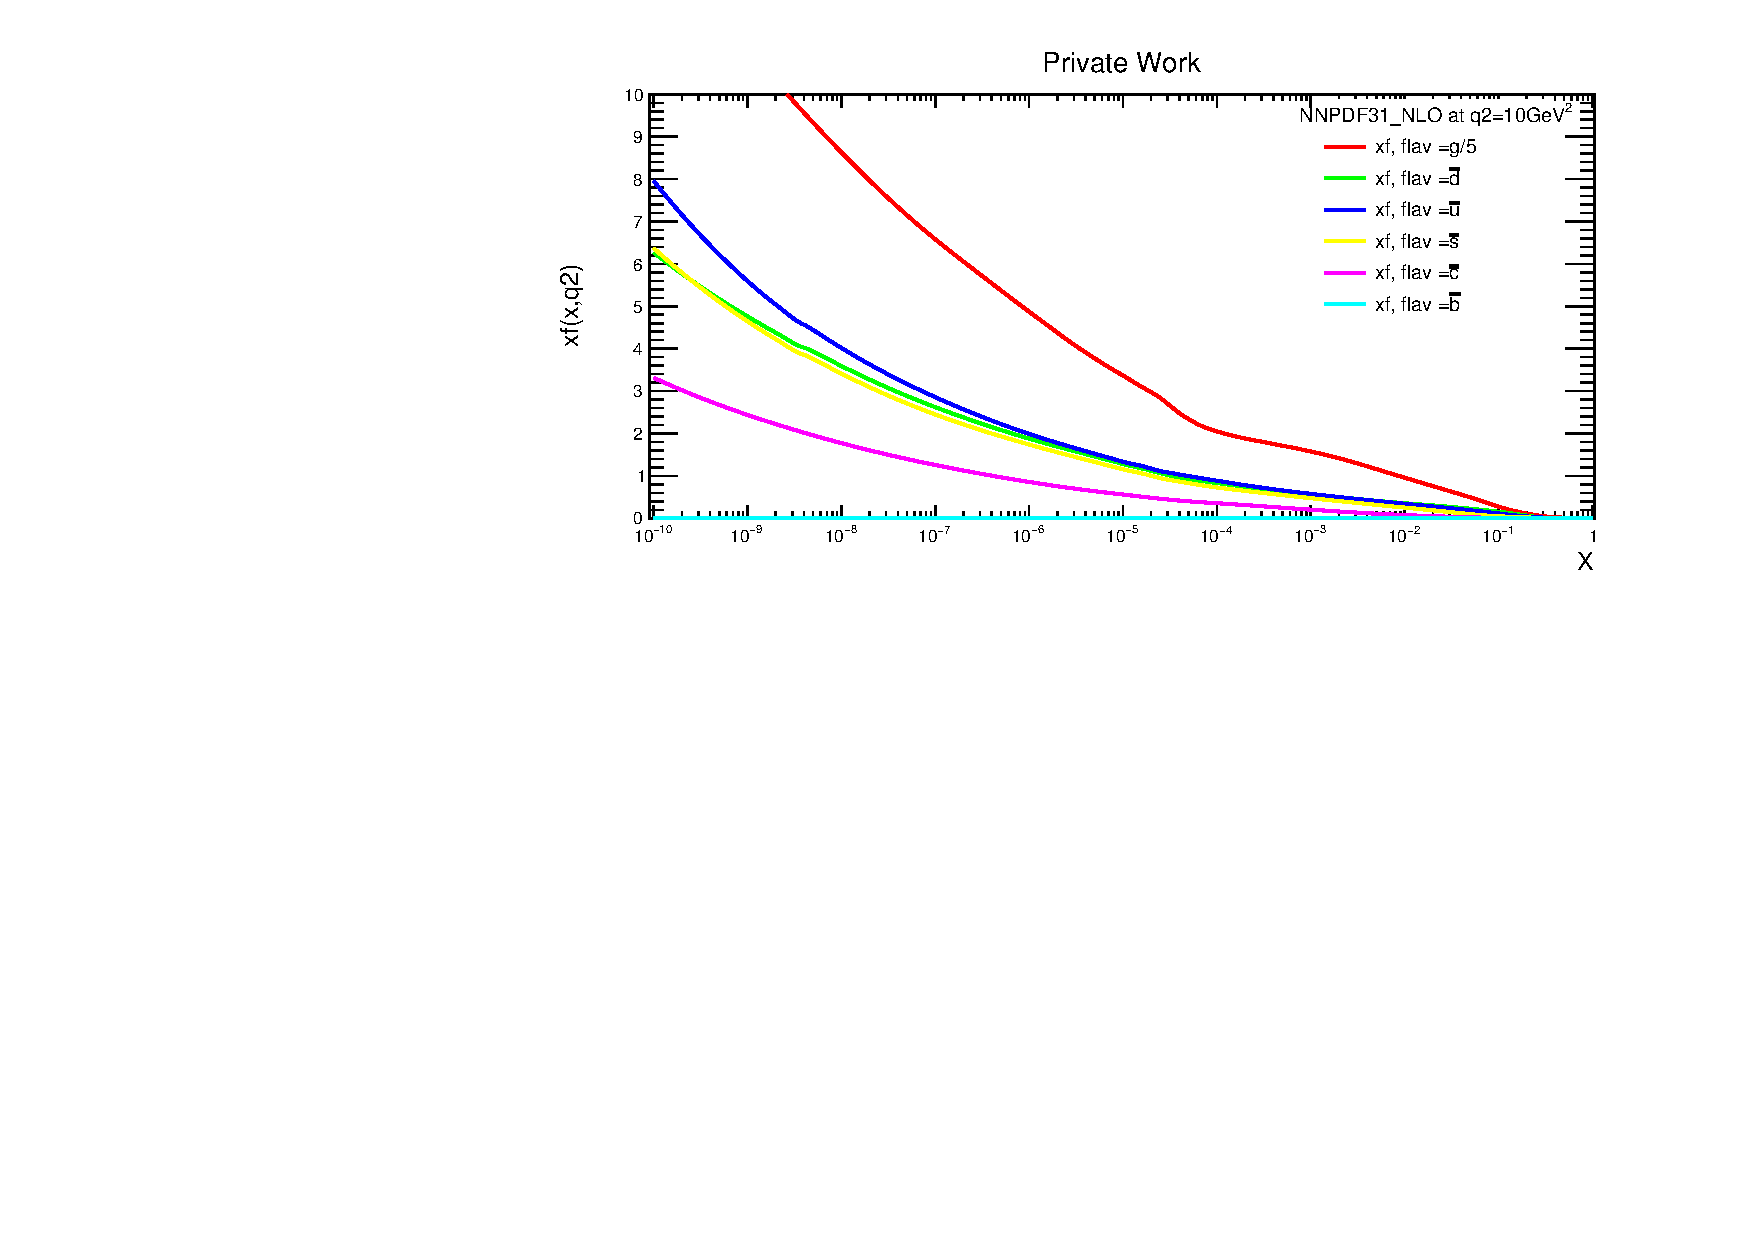
\includegraphics[height=5cm, width=\textwidth]{chapter4/barxfx10gev_nlo.pdf}
\vspace*{-8mm}
\caption{}
\end{subfigure}
\begin{subfigure}{0.45\textwidth}
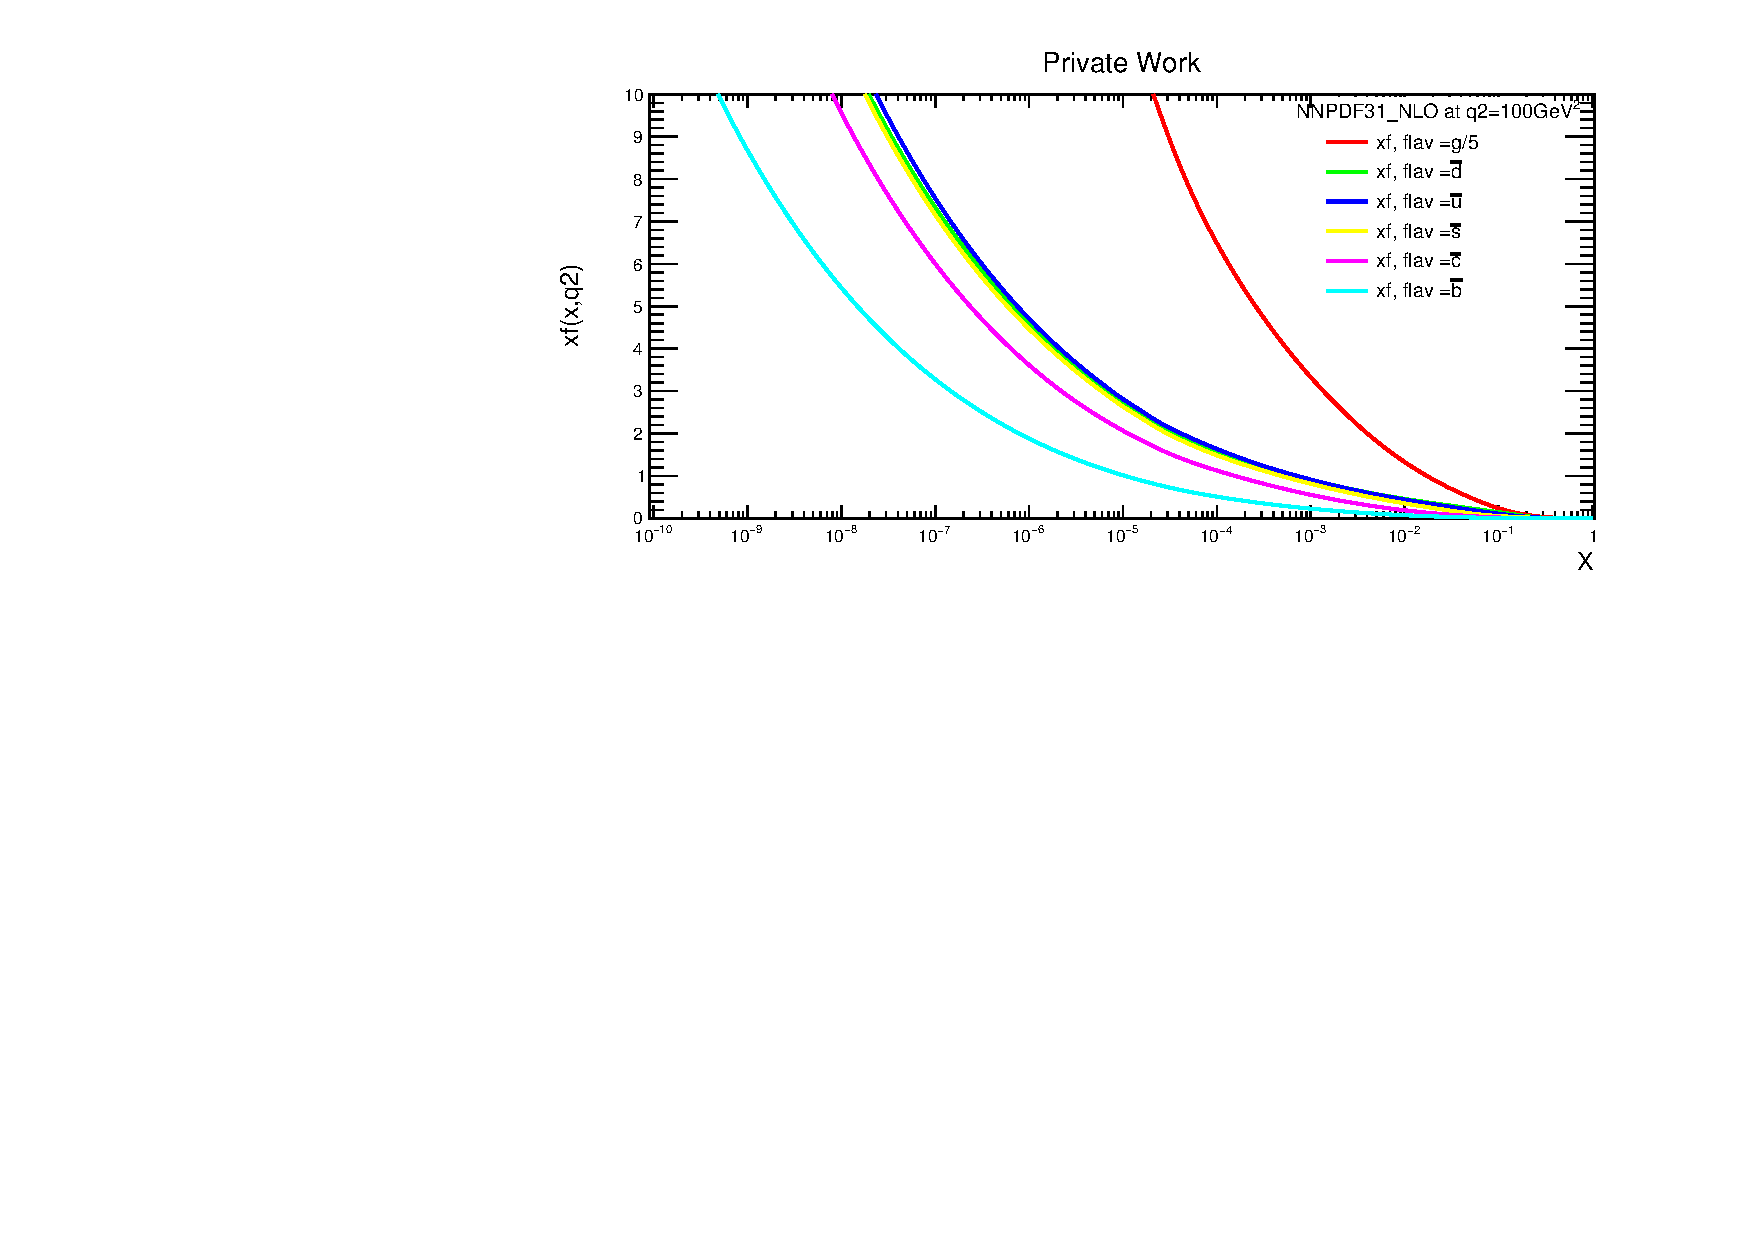
\includegraphics[height=5cm, width=\textwidth]{chapter4/barxfx100gev_nlo.pdf}
\vspace*{-8mm}
\caption{}
\end{subfigure}
\caption{The NNPDF3.1-NLO PDFs as a function of $x$ for the gluon~(g), down~(d),~up(u), strange~(s), charm~(c) and bottom~(b) quarks and also for the corresponding anti-quarks. (a), (b): for $Q^{2}= 10GeV^{2}$, (c), (d): for $Q^{2}=100GeV^{2}$ and (e), (f): for $Q^{2}=1000GeV^{2}$, (g), (H): for anti-quarks at $10GeV^{2}$ and $100GeV^{2}$ respectively.} 
\label{nnpdf_nlo}
\end{figure}

\begin{figure}[H]
\centering
\begin{subfigure}{0.45\textwidth}
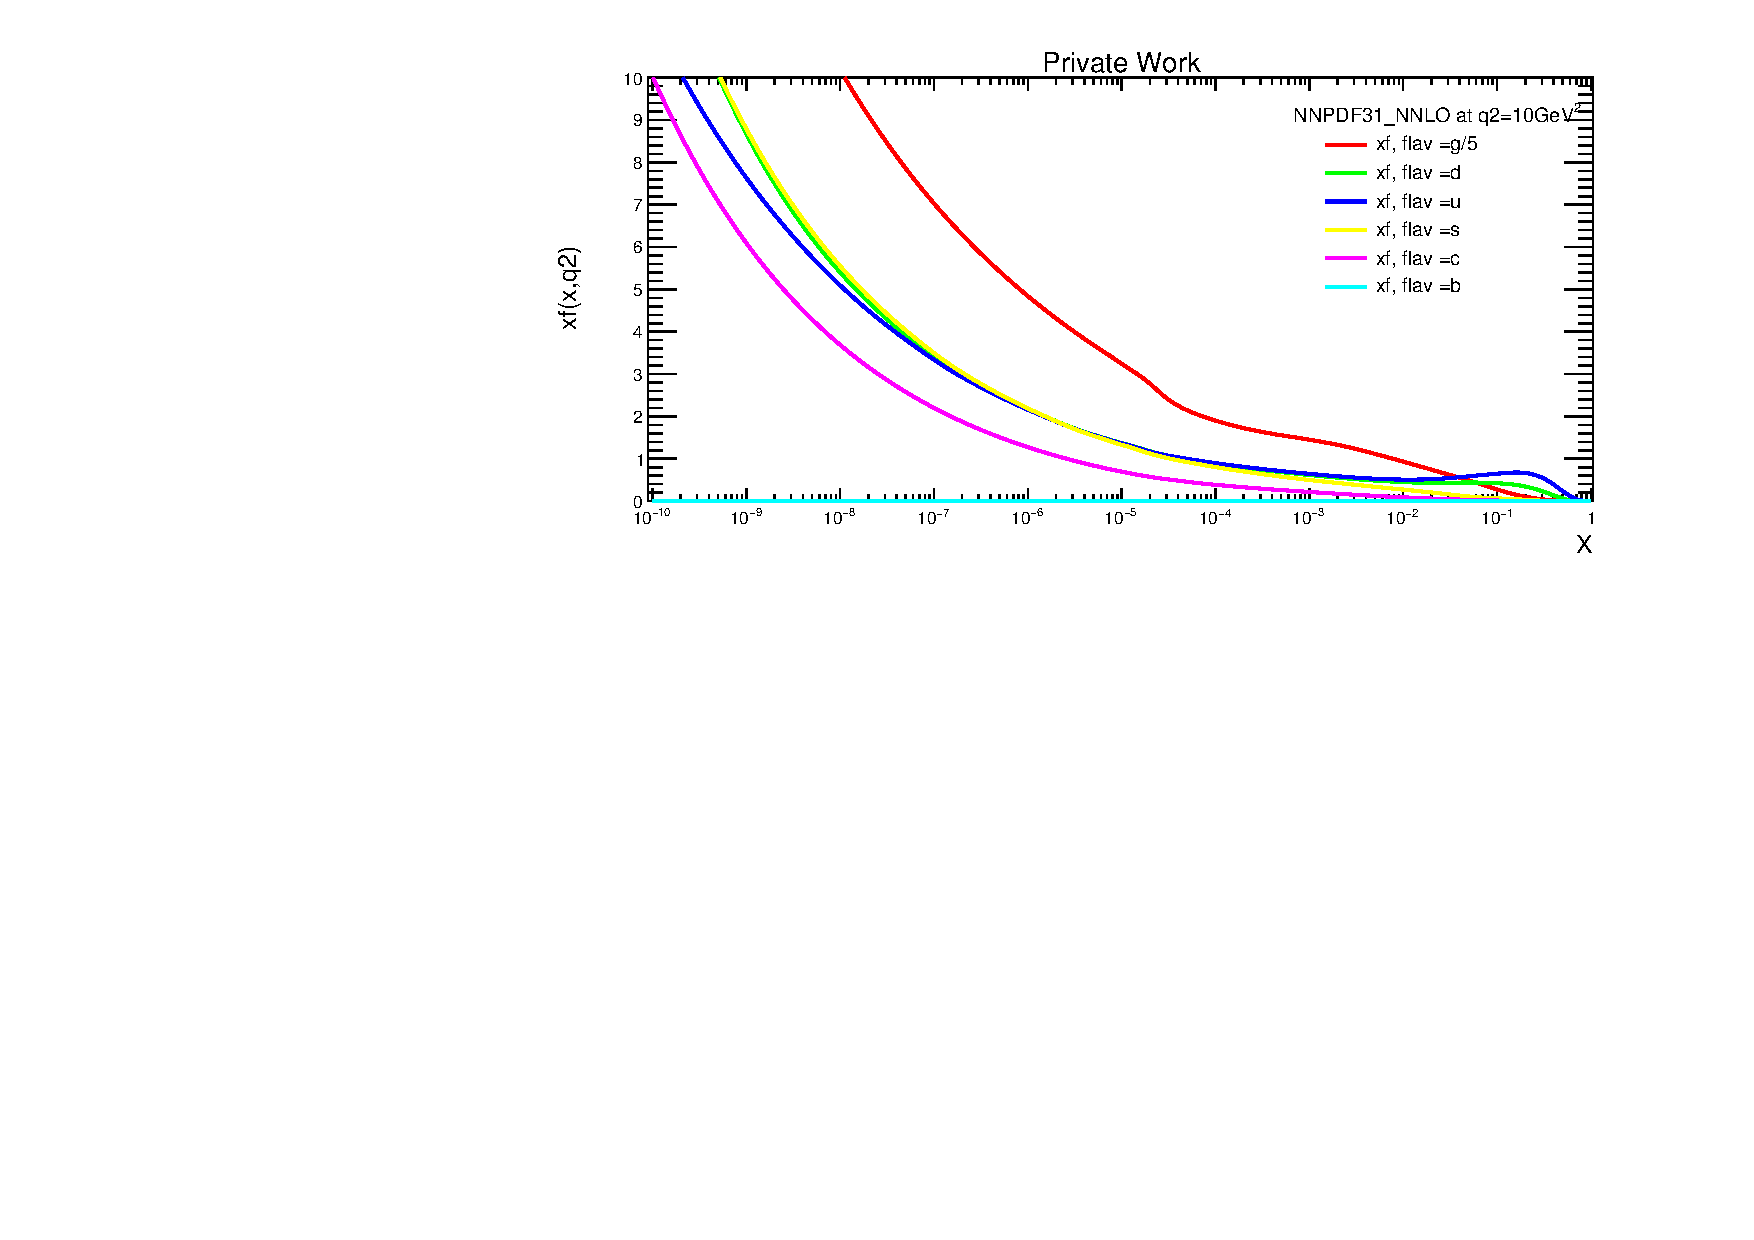
\includegraphics[height=5cm ,width=\textwidth]{chapter4/xfx10gev.pdf}
\vspace*{-8mm}
\caption{}
\end{subfigure}
\begin{subfigure}{0.45\textwidth}
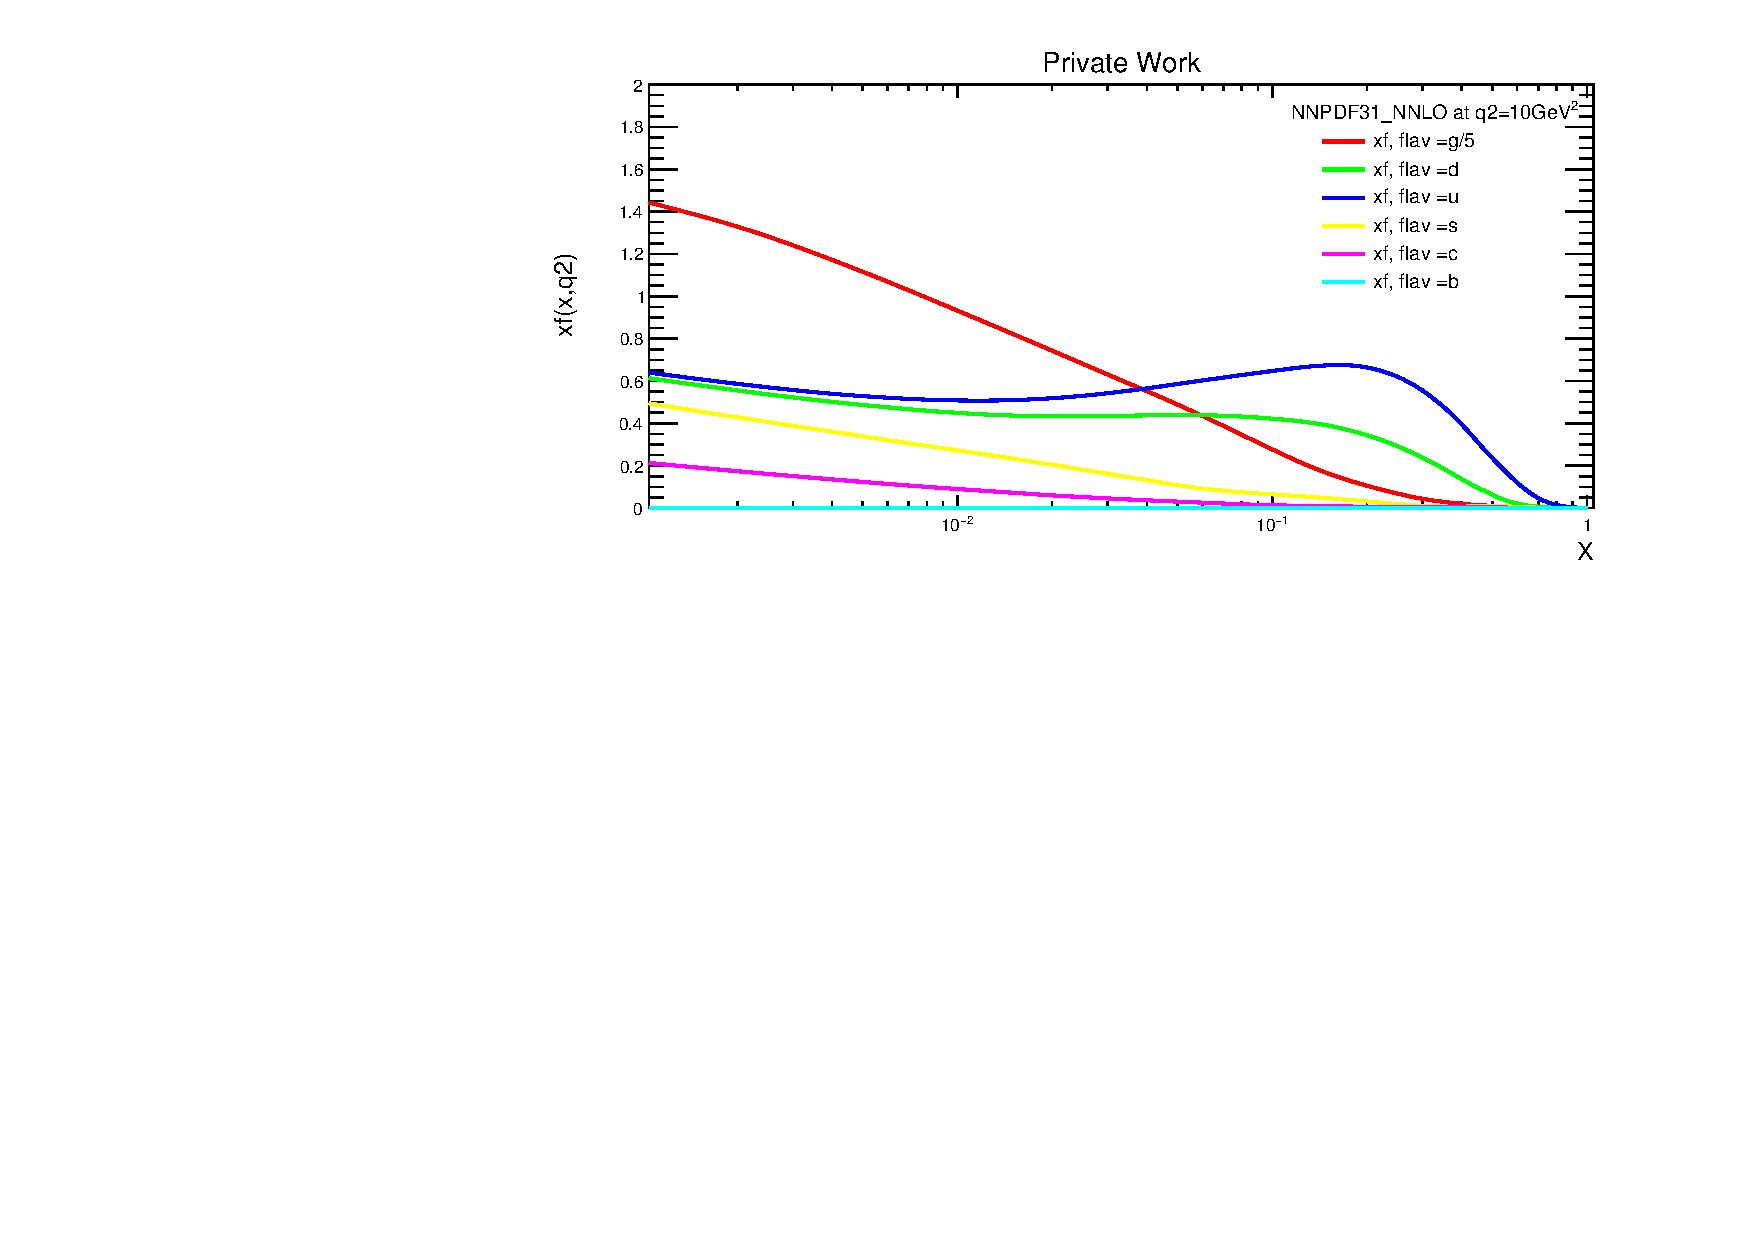
\includegraphics[height=5cm, width=\textwidth]{chapter4/xfx10gev1.pdf}
\vspace*{-8mm}
\caption{}
\end{subfigure}
\begin{subfigure}{0.45\textwidth}
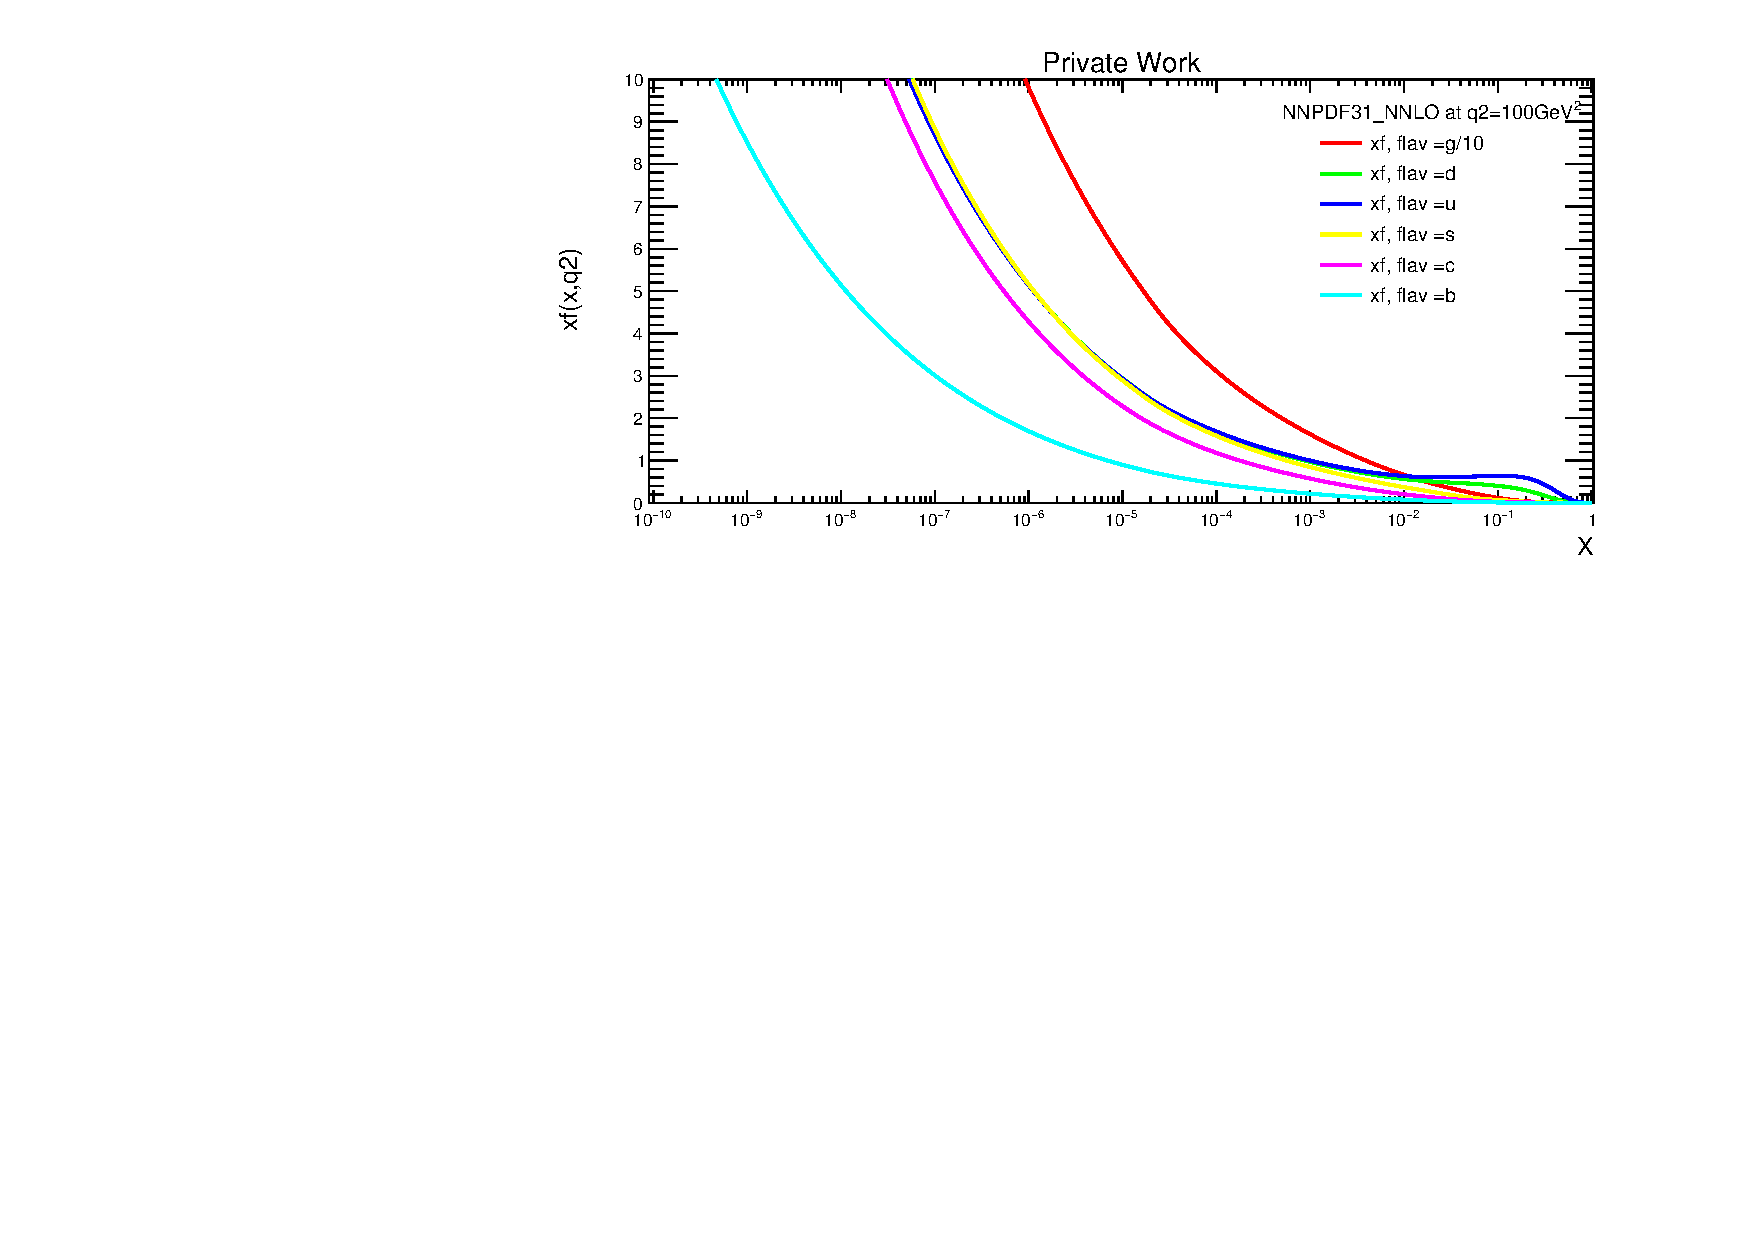
\includegraphics[height=5cm, width=\textwidth]{chapter4/xfx100gev.pdf}
\vspace*{-8mm}
\caption{}
\end{subfigure}
\begin{subfigure}{0.45\textwidth}
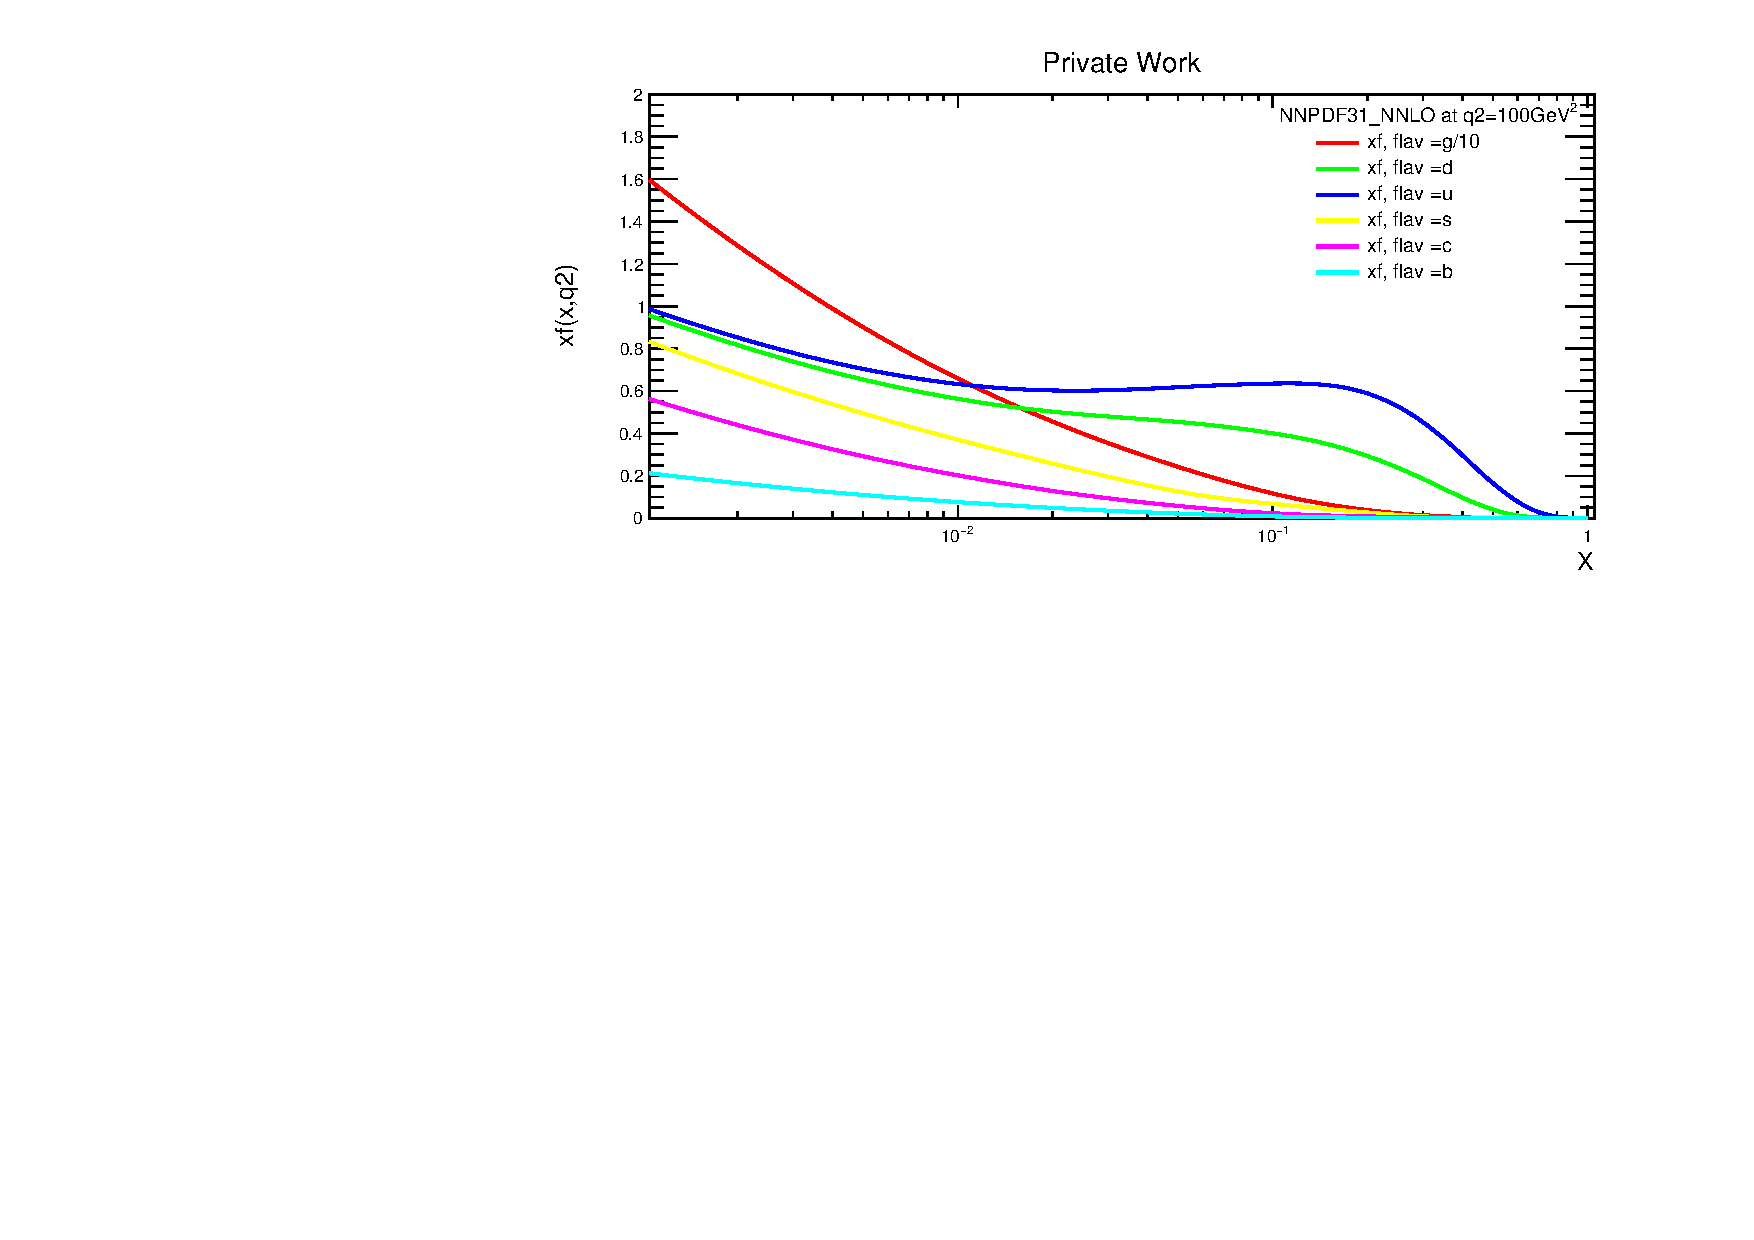
\includegraphics[height=5cm, width=\textwidth]{chapter4/xfx100gev1.pdf}
\vspace*{-8mm}
\caption{}
\end{subfigure}
\begin{subfigure}{0.45\textwidth}
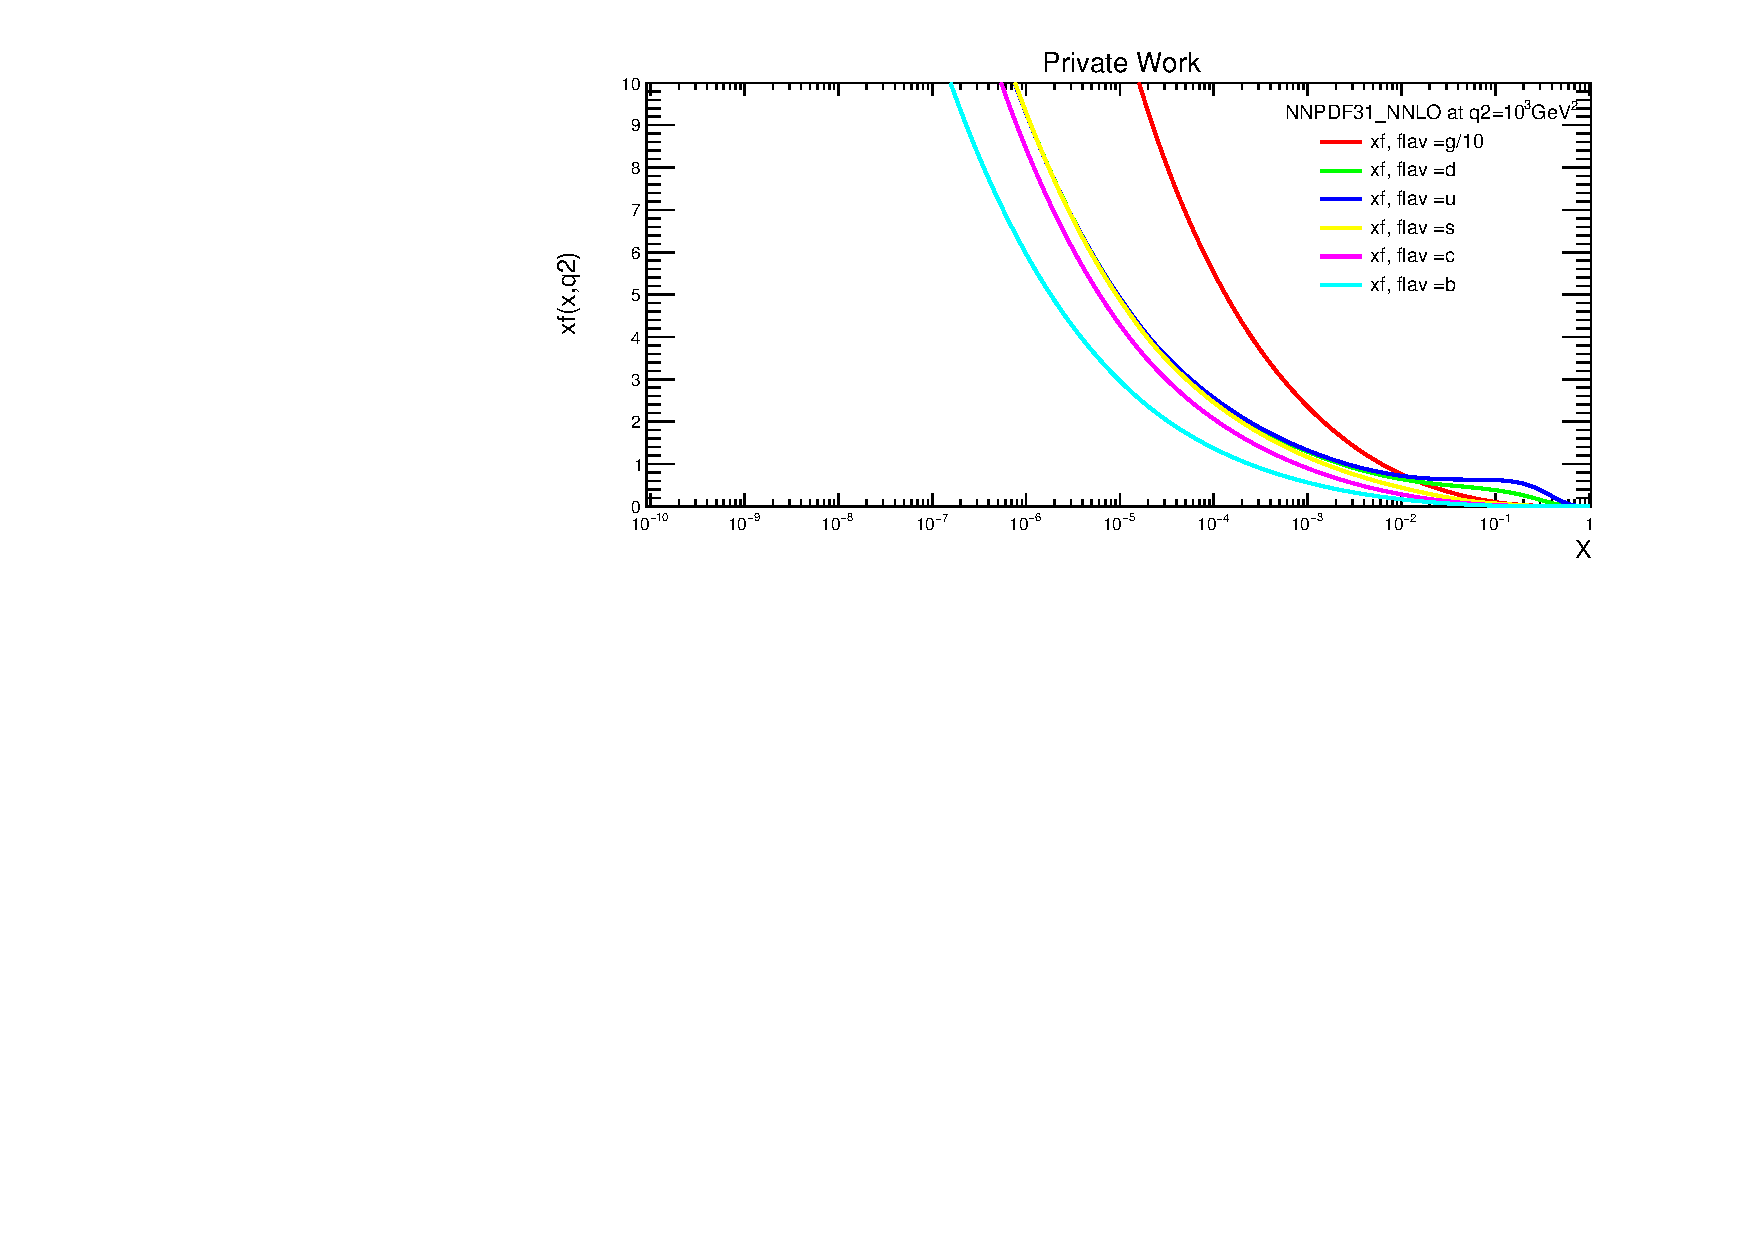
\includegraphics[height=5cm, width=\textwidth]{chapter4/xfx1000gev.pdf}
\vspace*{-8mm}
\caption{}
\end{subfigure}
\begin{subfigure}{0.45\textwidth}
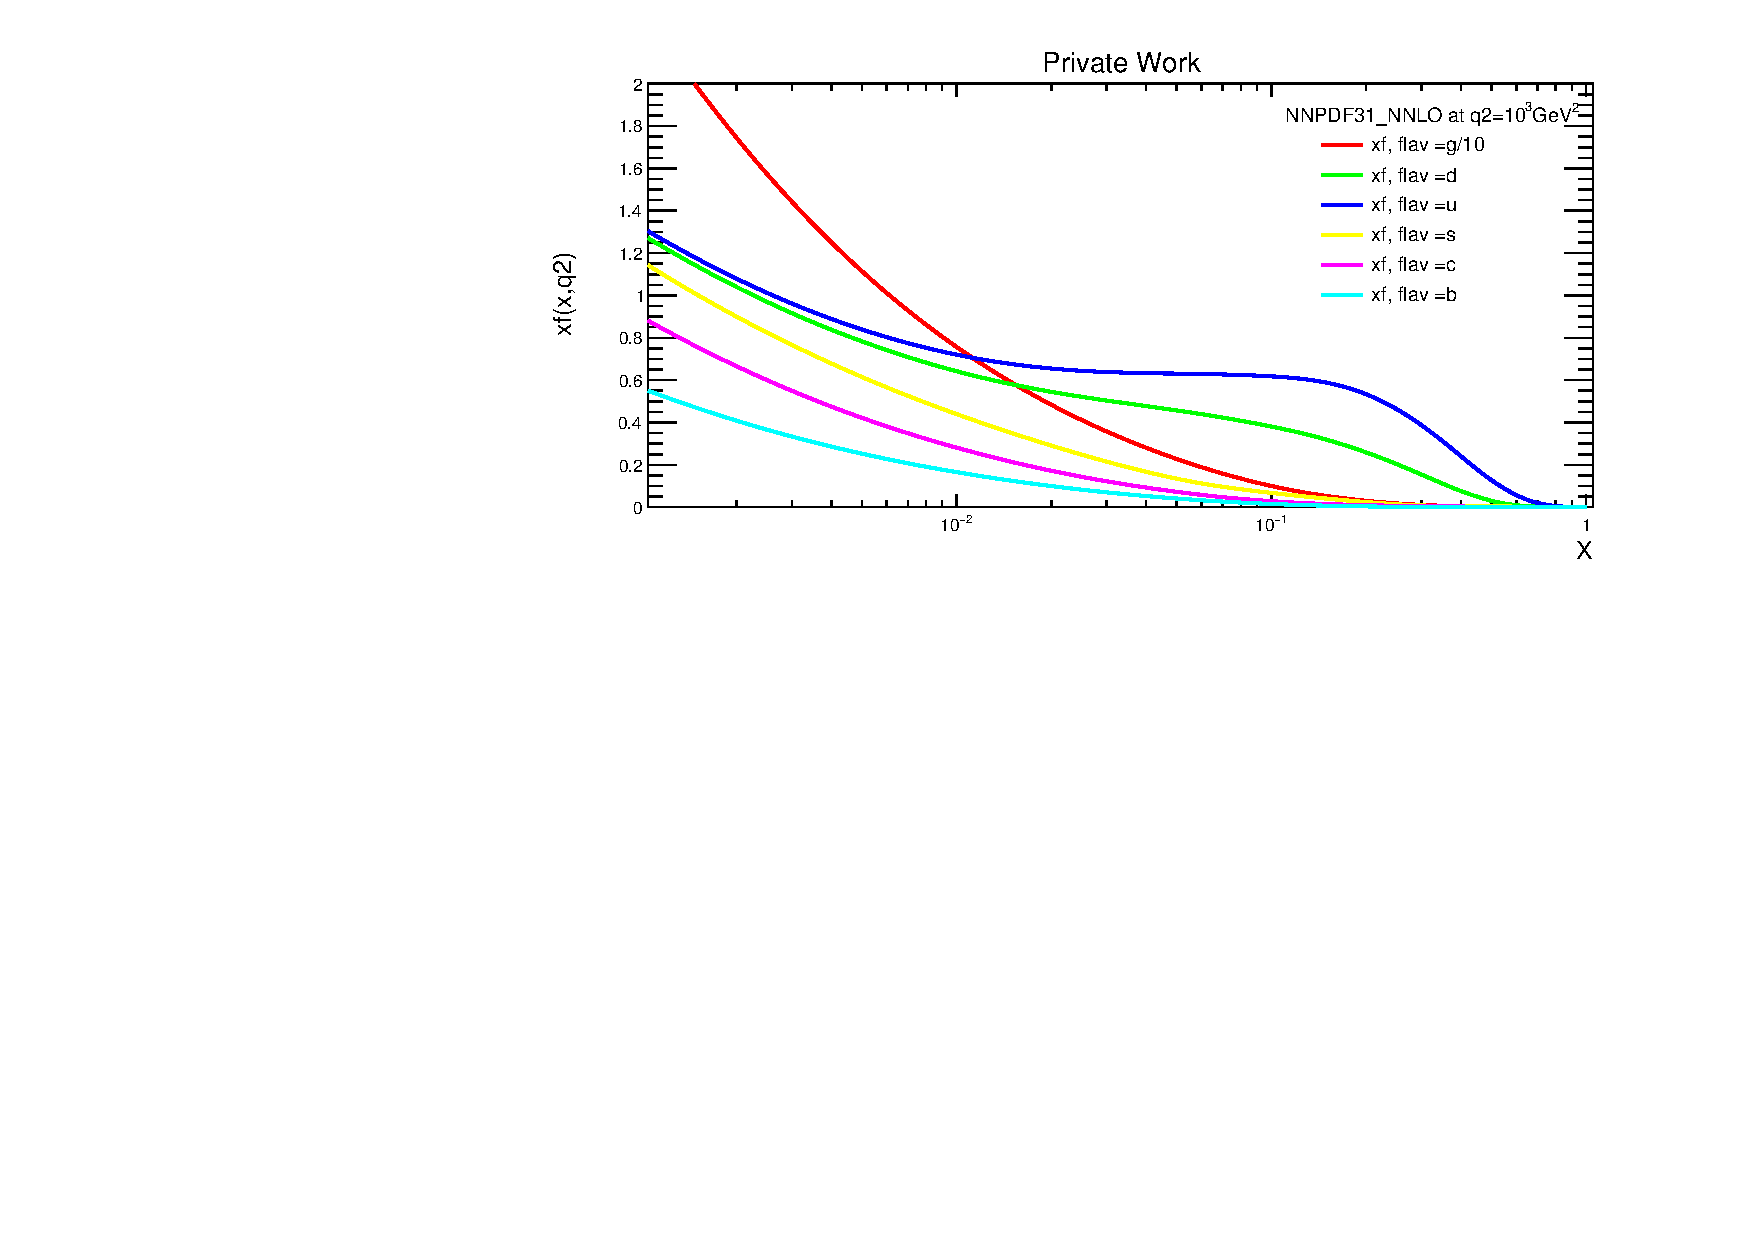
\includegraphics[height=5cm, width=\textwidth]{chapter4/xfx1000gev1.pdf}
\vspace*{-8mm}
\caption{}
\end{subfigure}
\begin{subfigure}{0.45\textwidth}
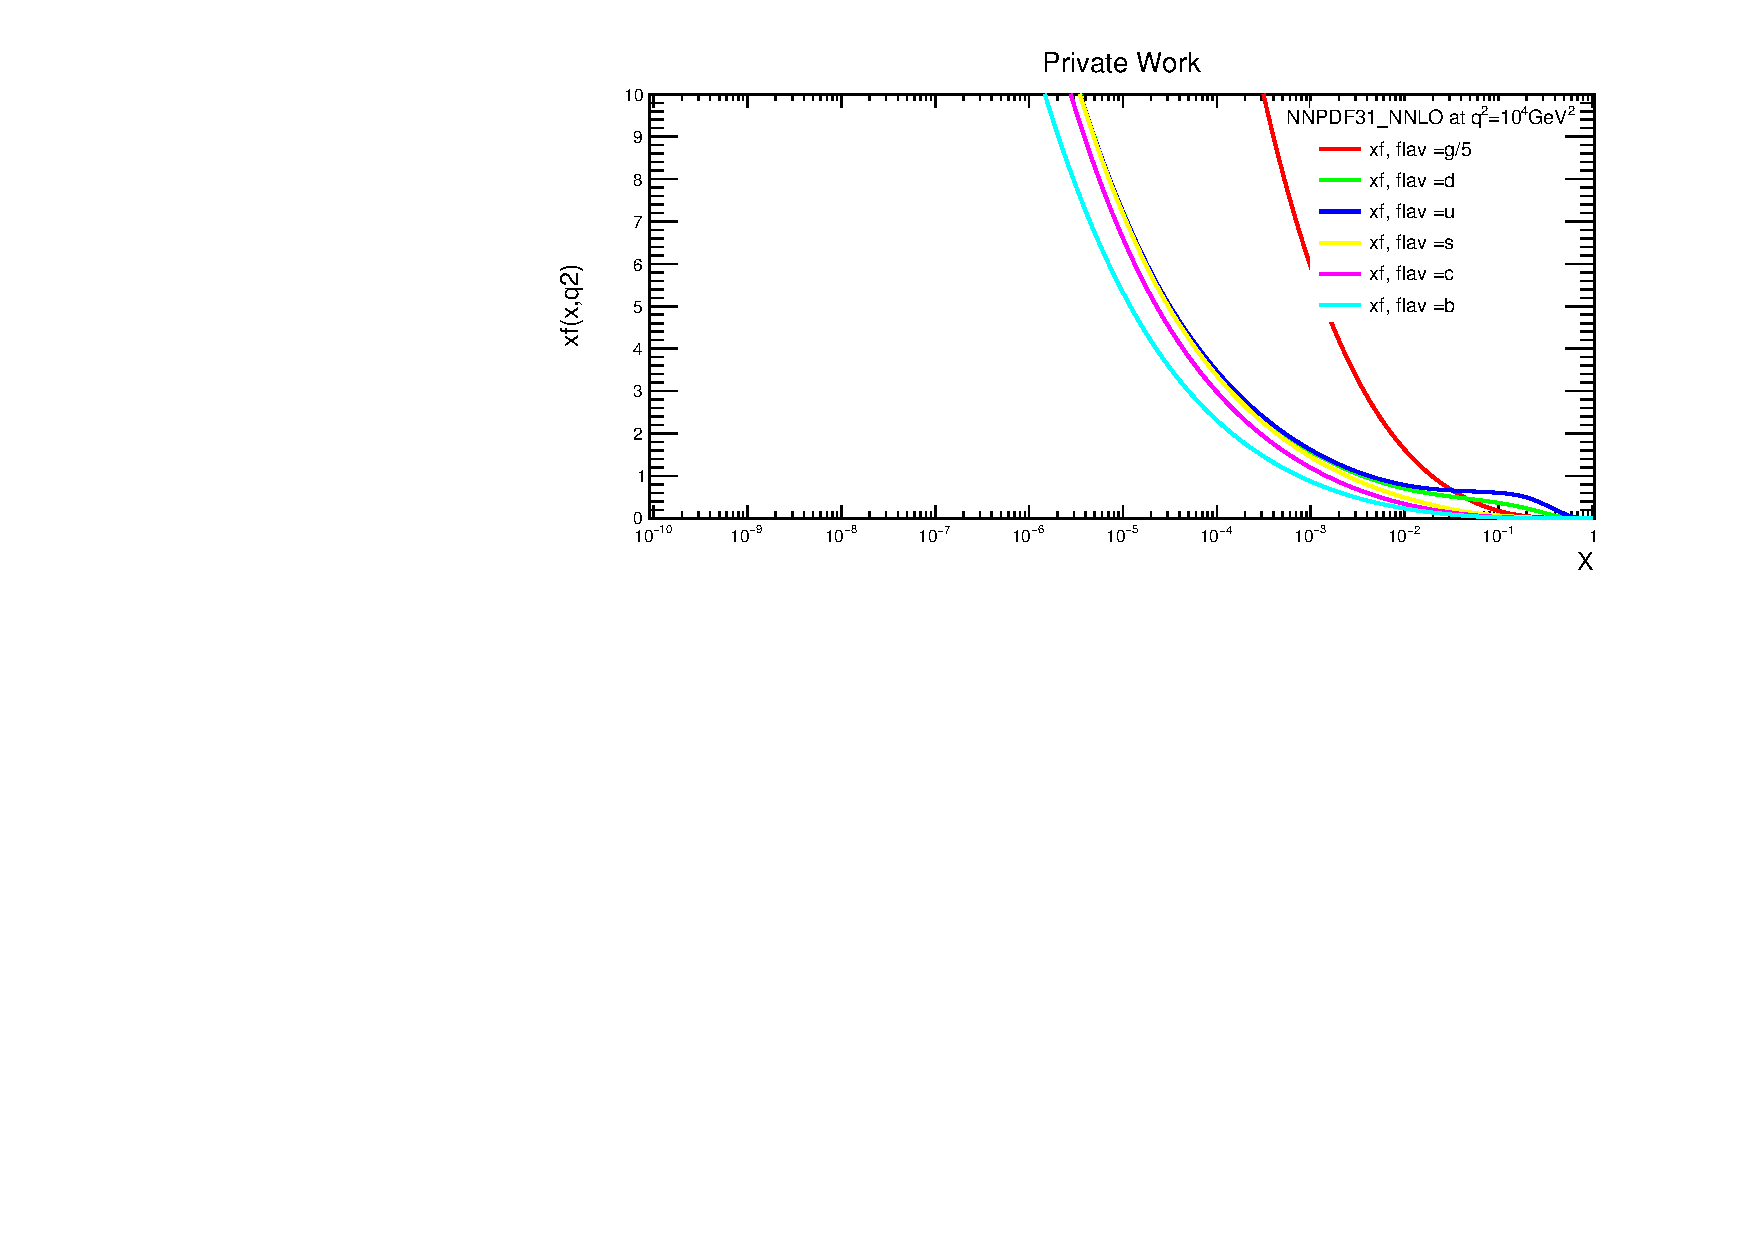
\includegraphics[height=5cm, width=\textwidth]{chapter4/xfx10000gev.pdf}
\vspace*{-8mm}
\caption{}
\end{subfigure}
\begin{subfigure}{0.45\textwidth}
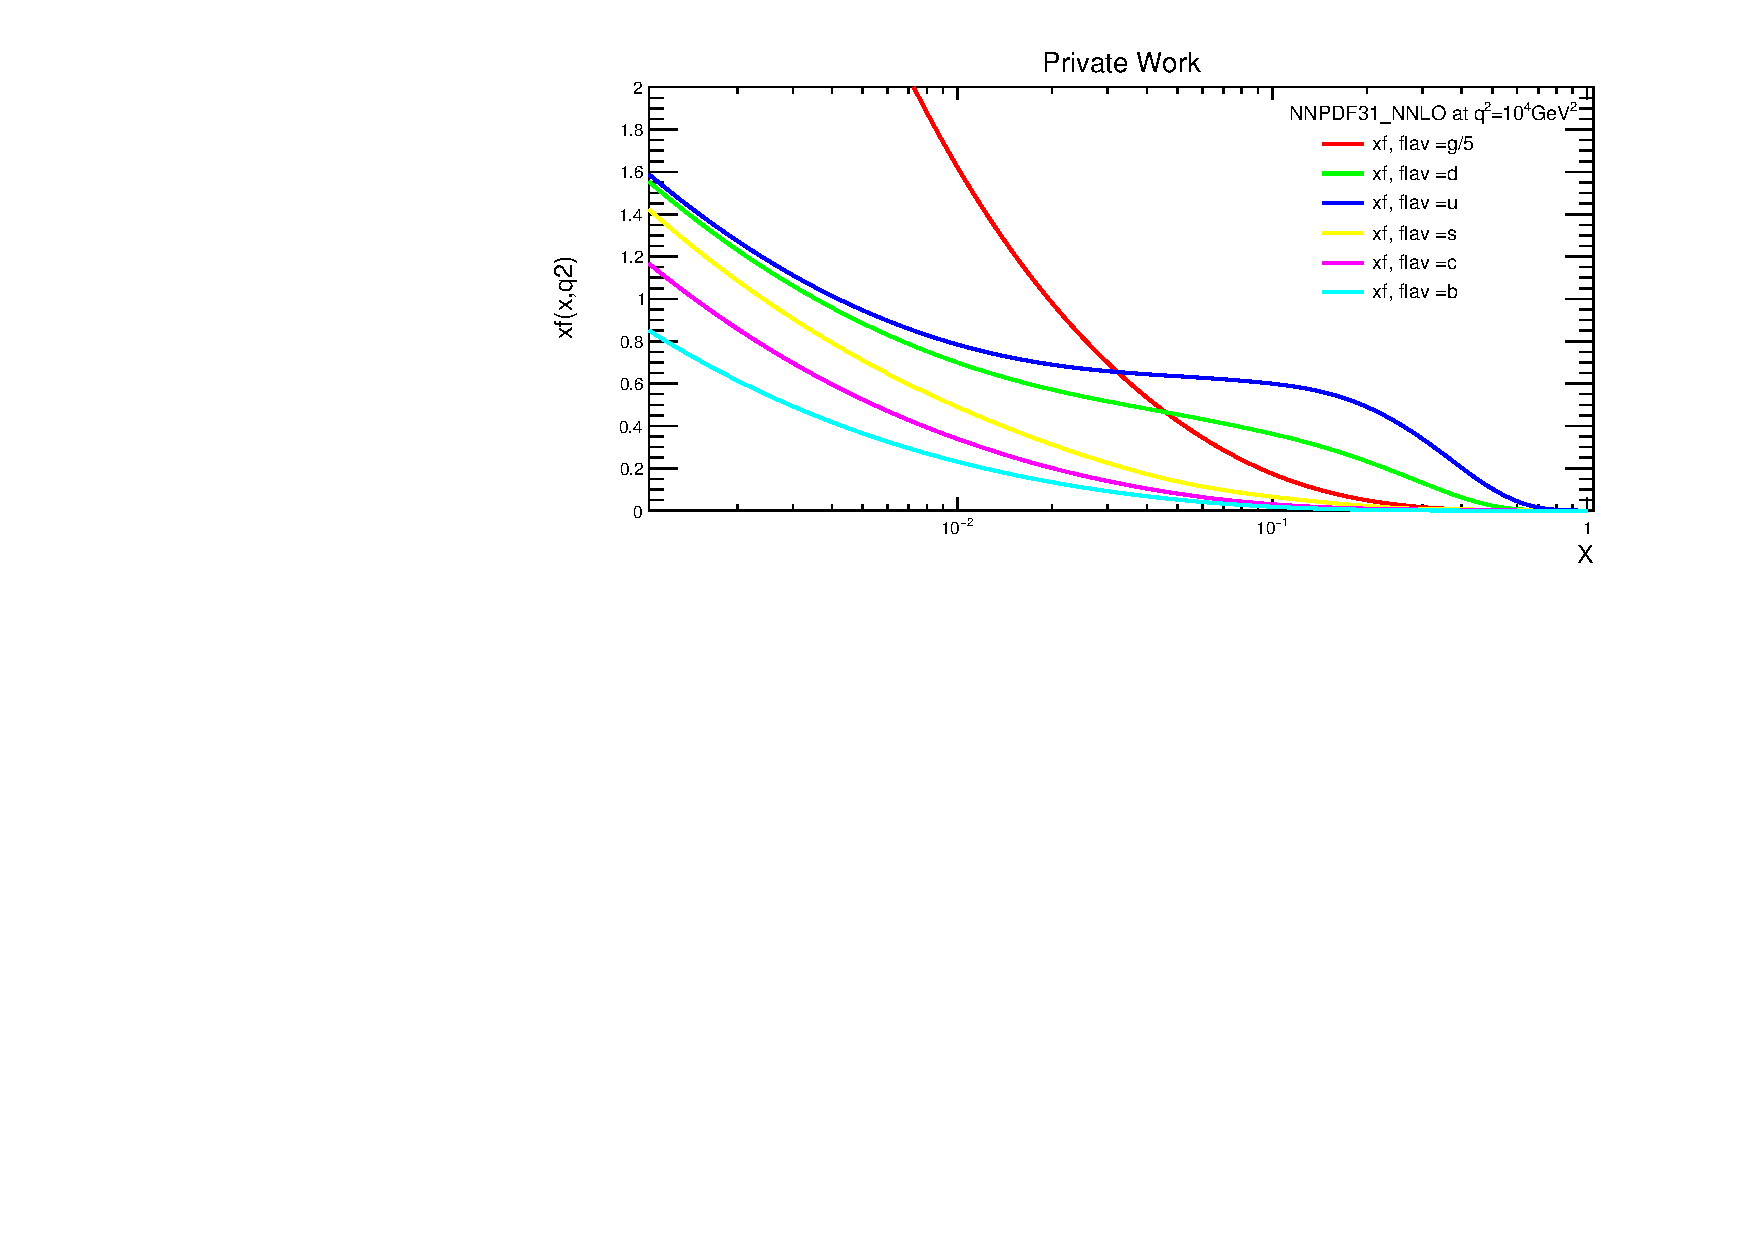
\includegraphics[height=5cm, width=\textwidth]{chapter4/xfx10000gev1.pdf}
\vspace*{-8mm}
\caption{}
\end{subfigure}
\caption{The NNPDF3.1-NNLO PDFs as a function of $x$ for the gluon~(g), down~(d),~up(u), strange~(s), charm~(c) and bottom~(b) quarks. (a), (b): for $Q^{2}= 10GeV^{2}$, (c), (d): for $Q^{2}=100GeV^{2}$ and (e), (f): for $Q^{2}=1000GeV^{2}$, (g), (h): for $10000GeV^{2}$. The gluon PDFs are scaled down by a factor of 5 and 10.} 
\label{nnpdf_nnlo}
\end{figure}

\begin{figure}[H]
\centering
\begin{subfigure}{0.45\textwidth}
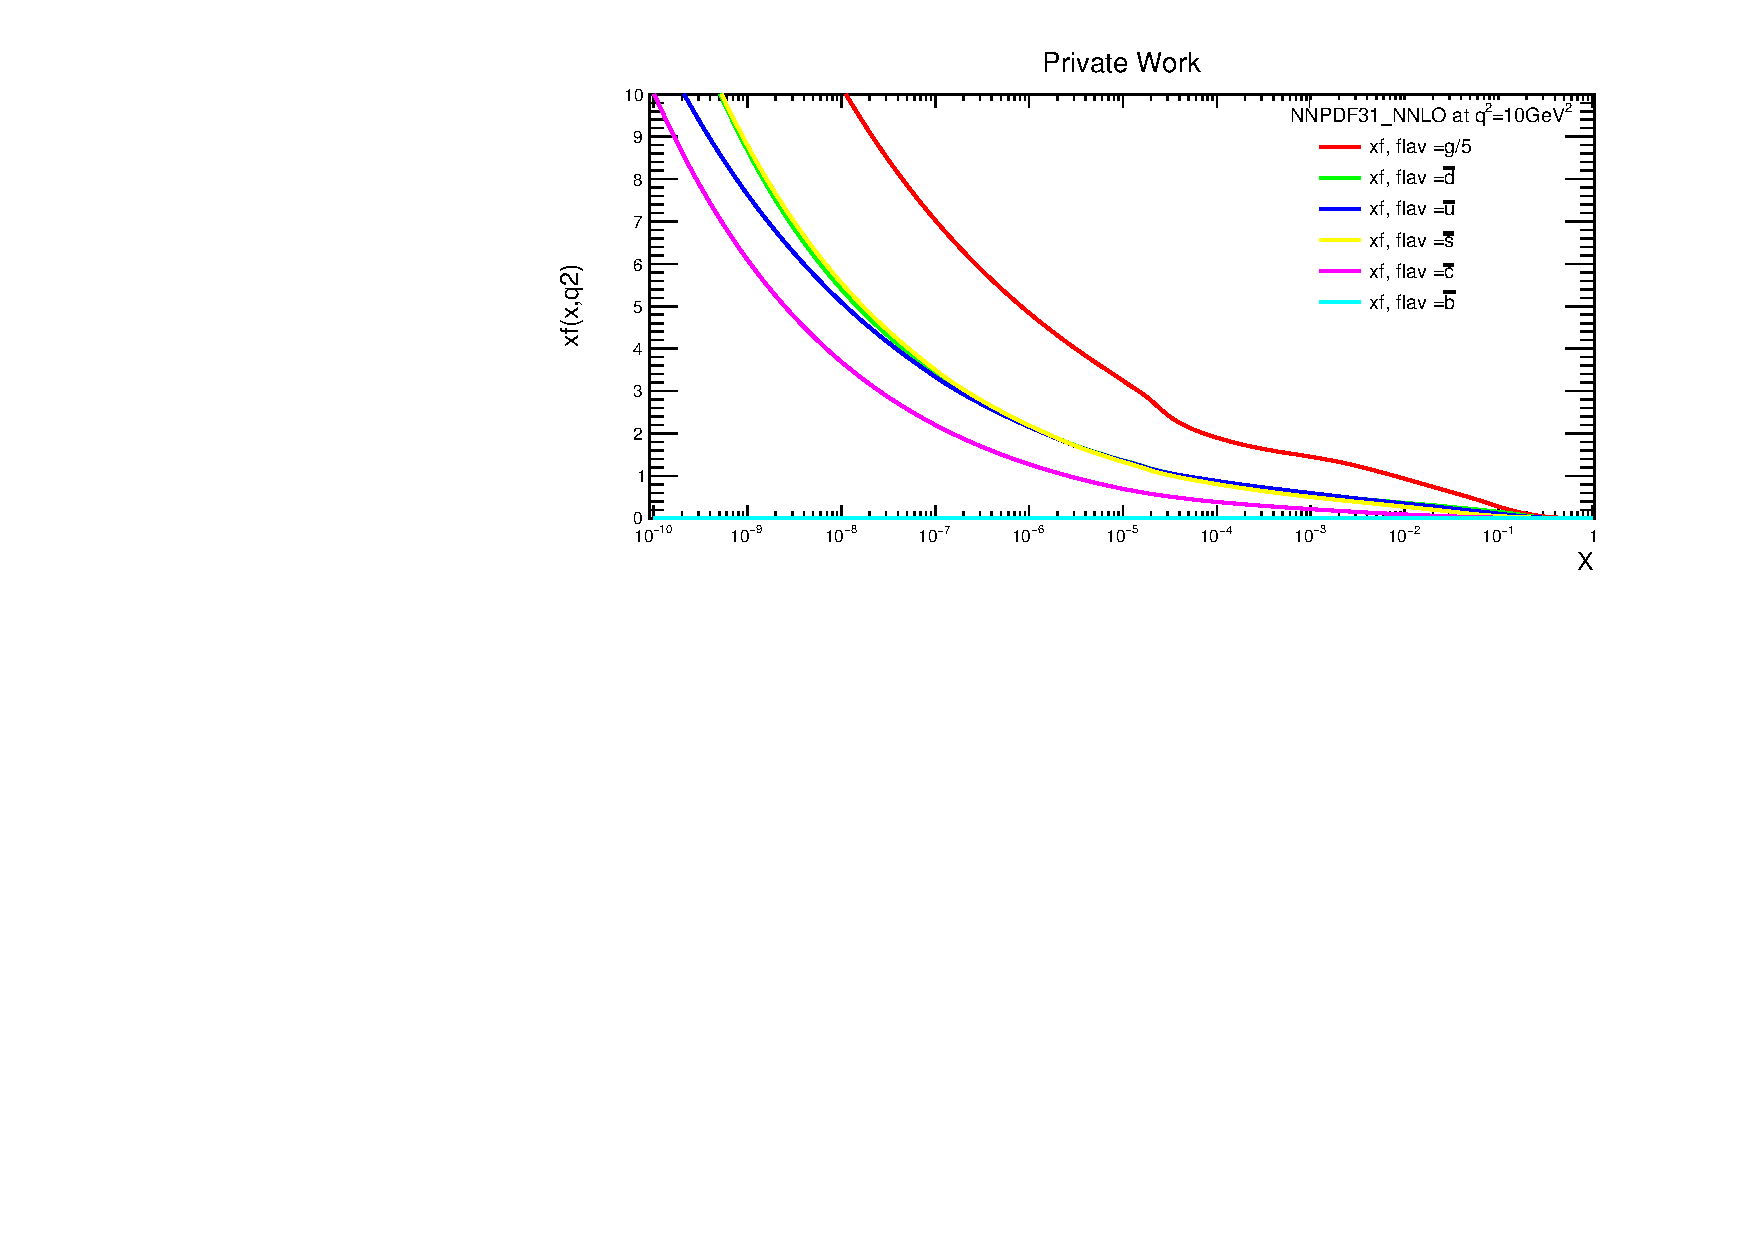
\includegraphics[height=5cm ,width=\textwidth]{chapter4/barxfx10gev.pdf}
\vspace*{-8mm}
\caption{}
\end{subfigure}
\begin{subfigure}{0.45\textwidth}
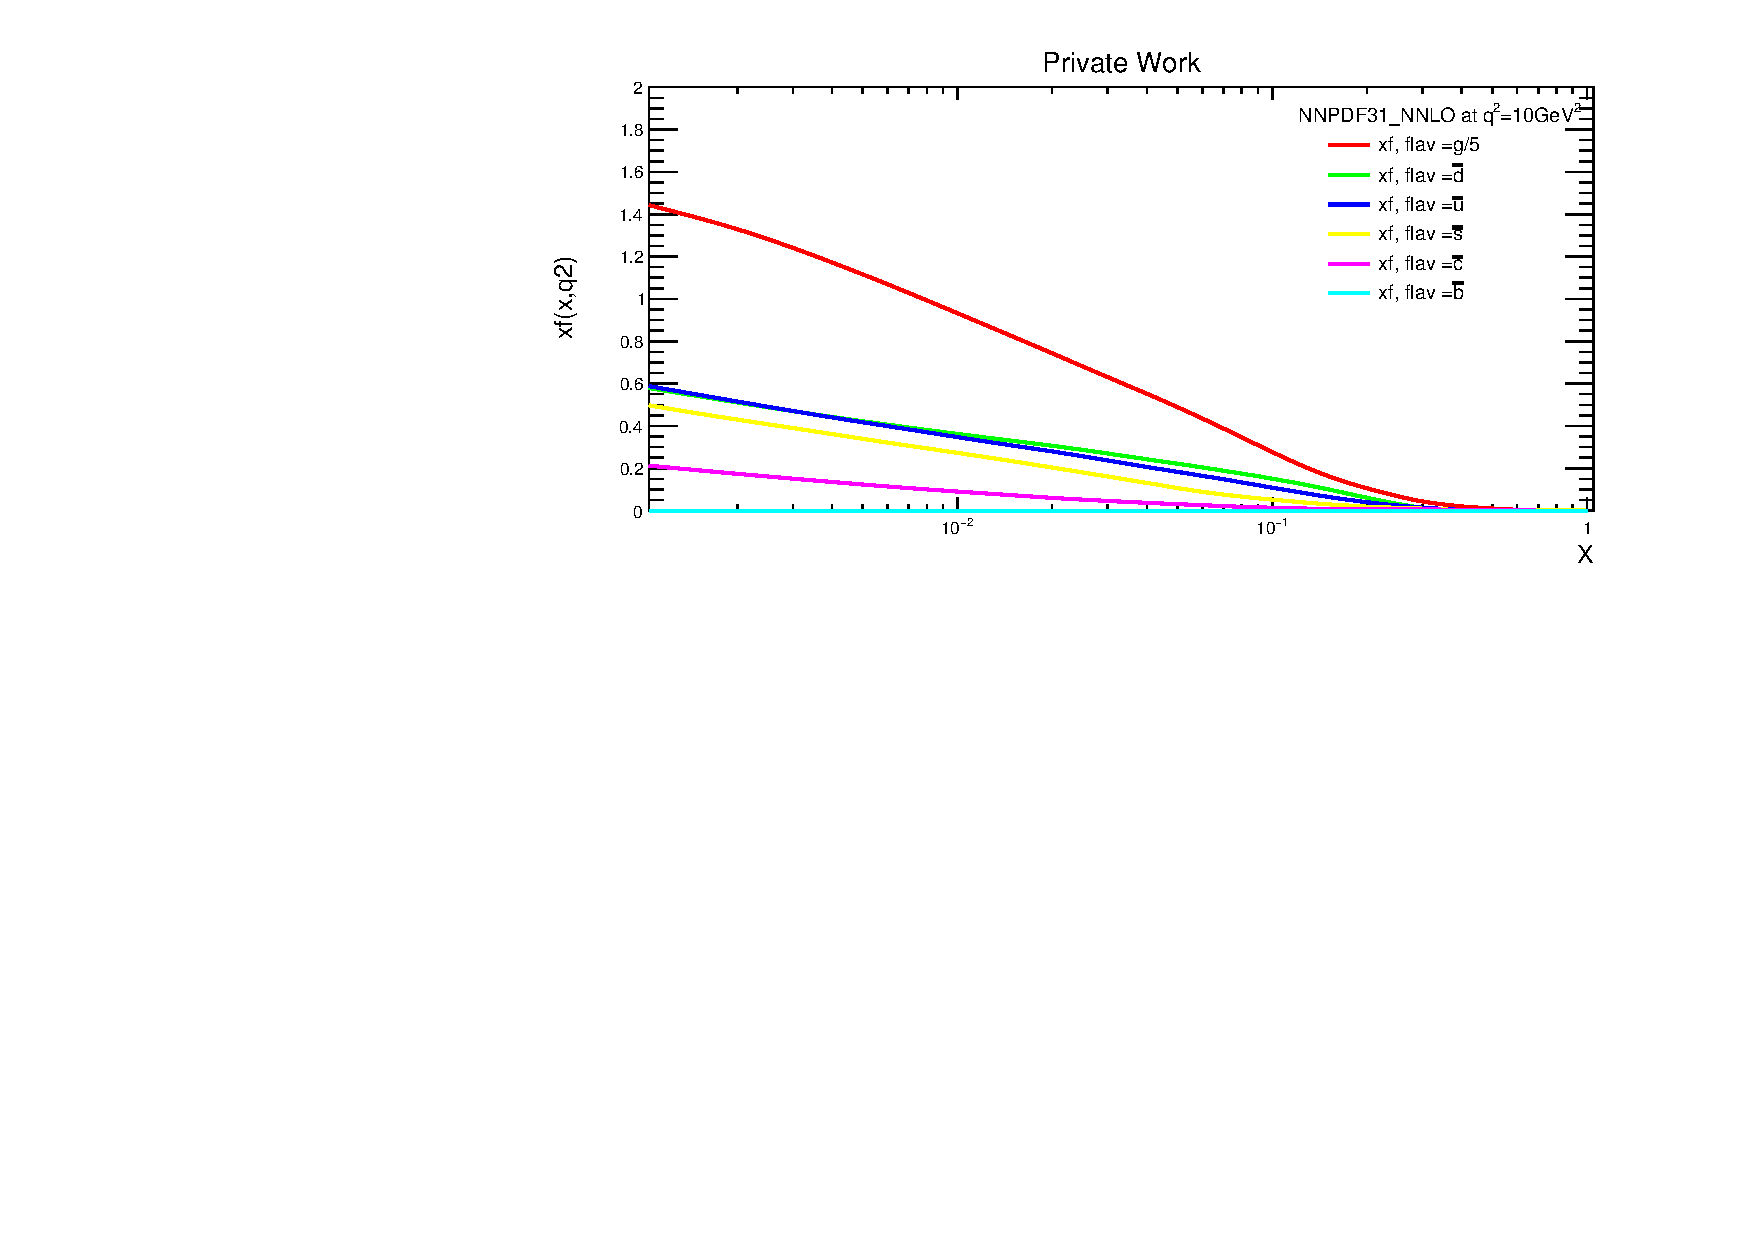
\includegraphics[height=5cm, width=\textwidth]{chapter4/barxfx10gev1.pdf}
\vspace*{-8mm}
\caption{}
\end{subfigure}
\begin{subfigure}{0.45\textwidth}
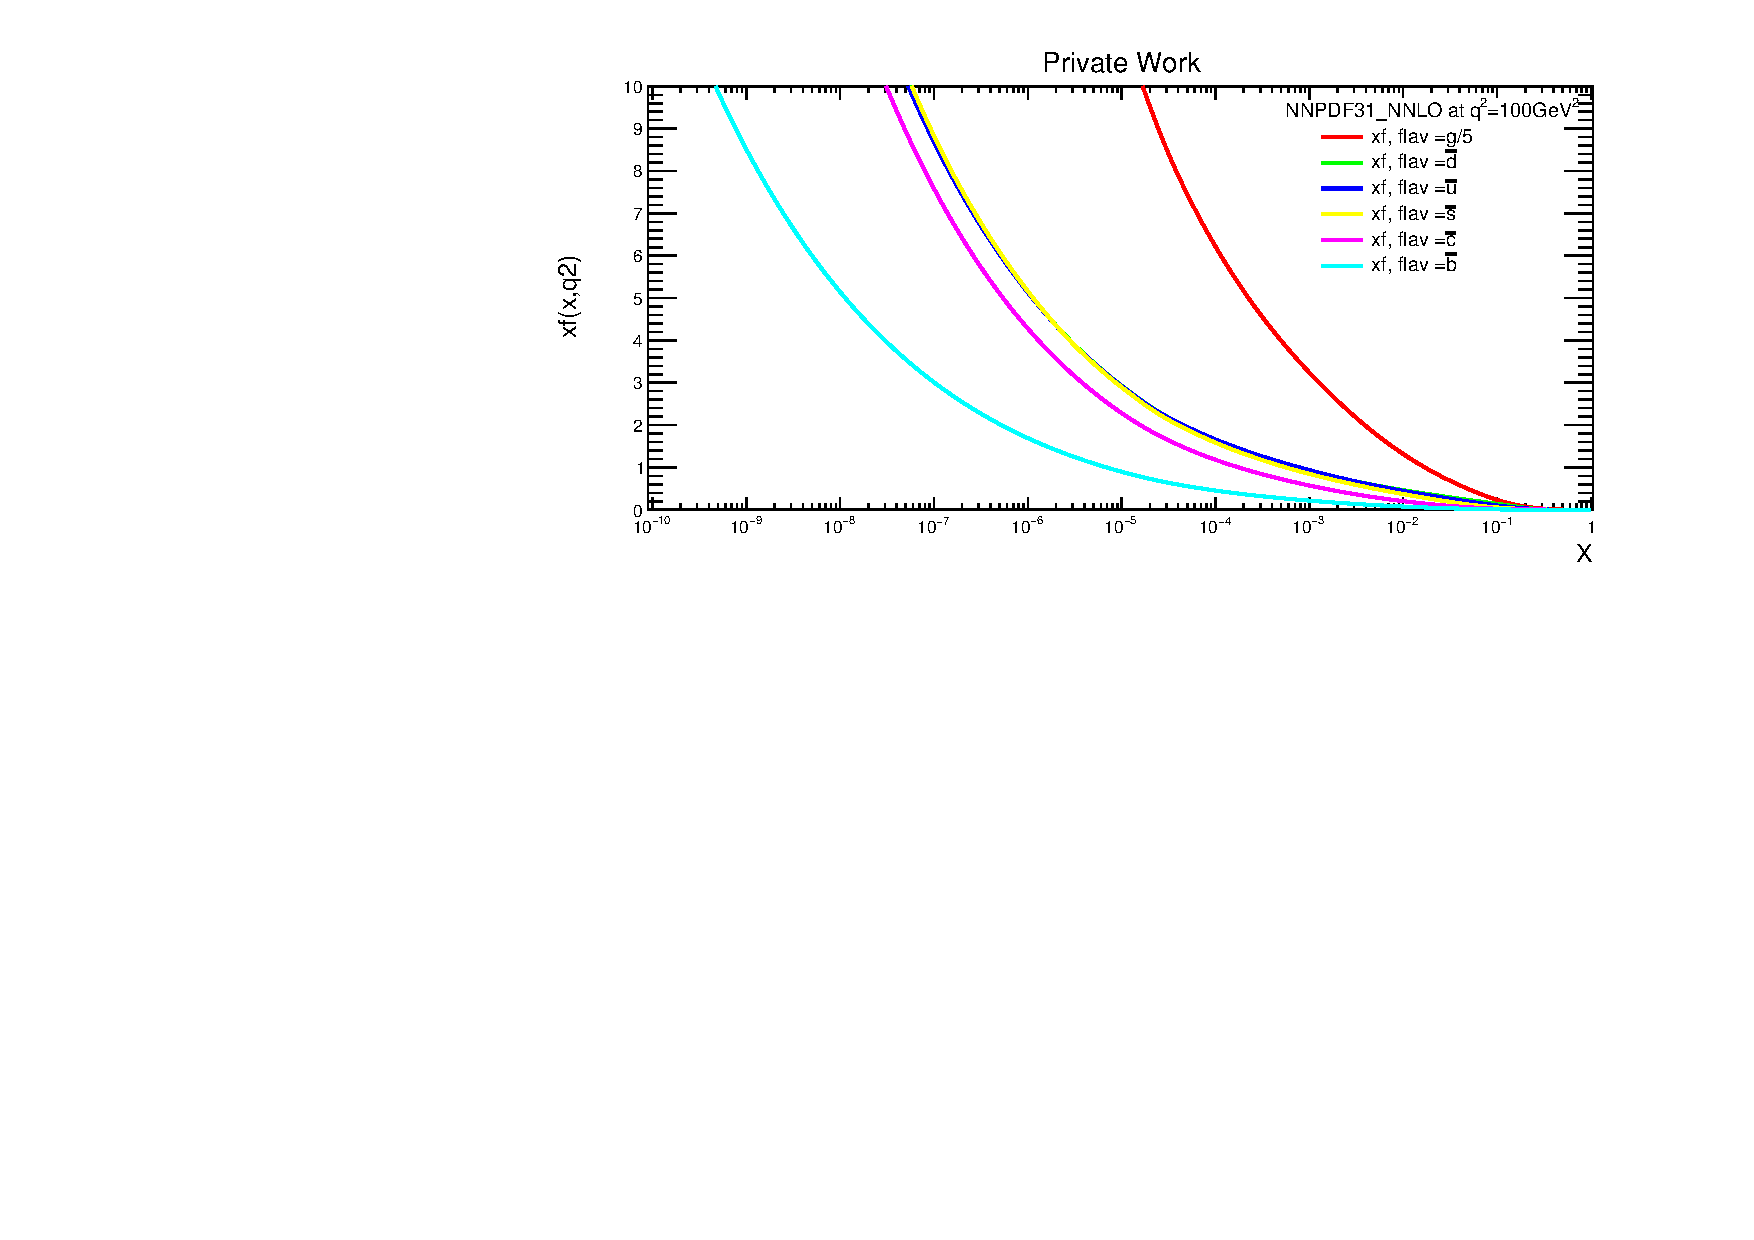
\includegraphics[height=5cm, width=\textwidth]{chapter4/barxfx100gev.pdf}
\vspace*{-8mm}
\caption{}
\end{subfigure}
\begin{subfigure}{0.45\textwidth}
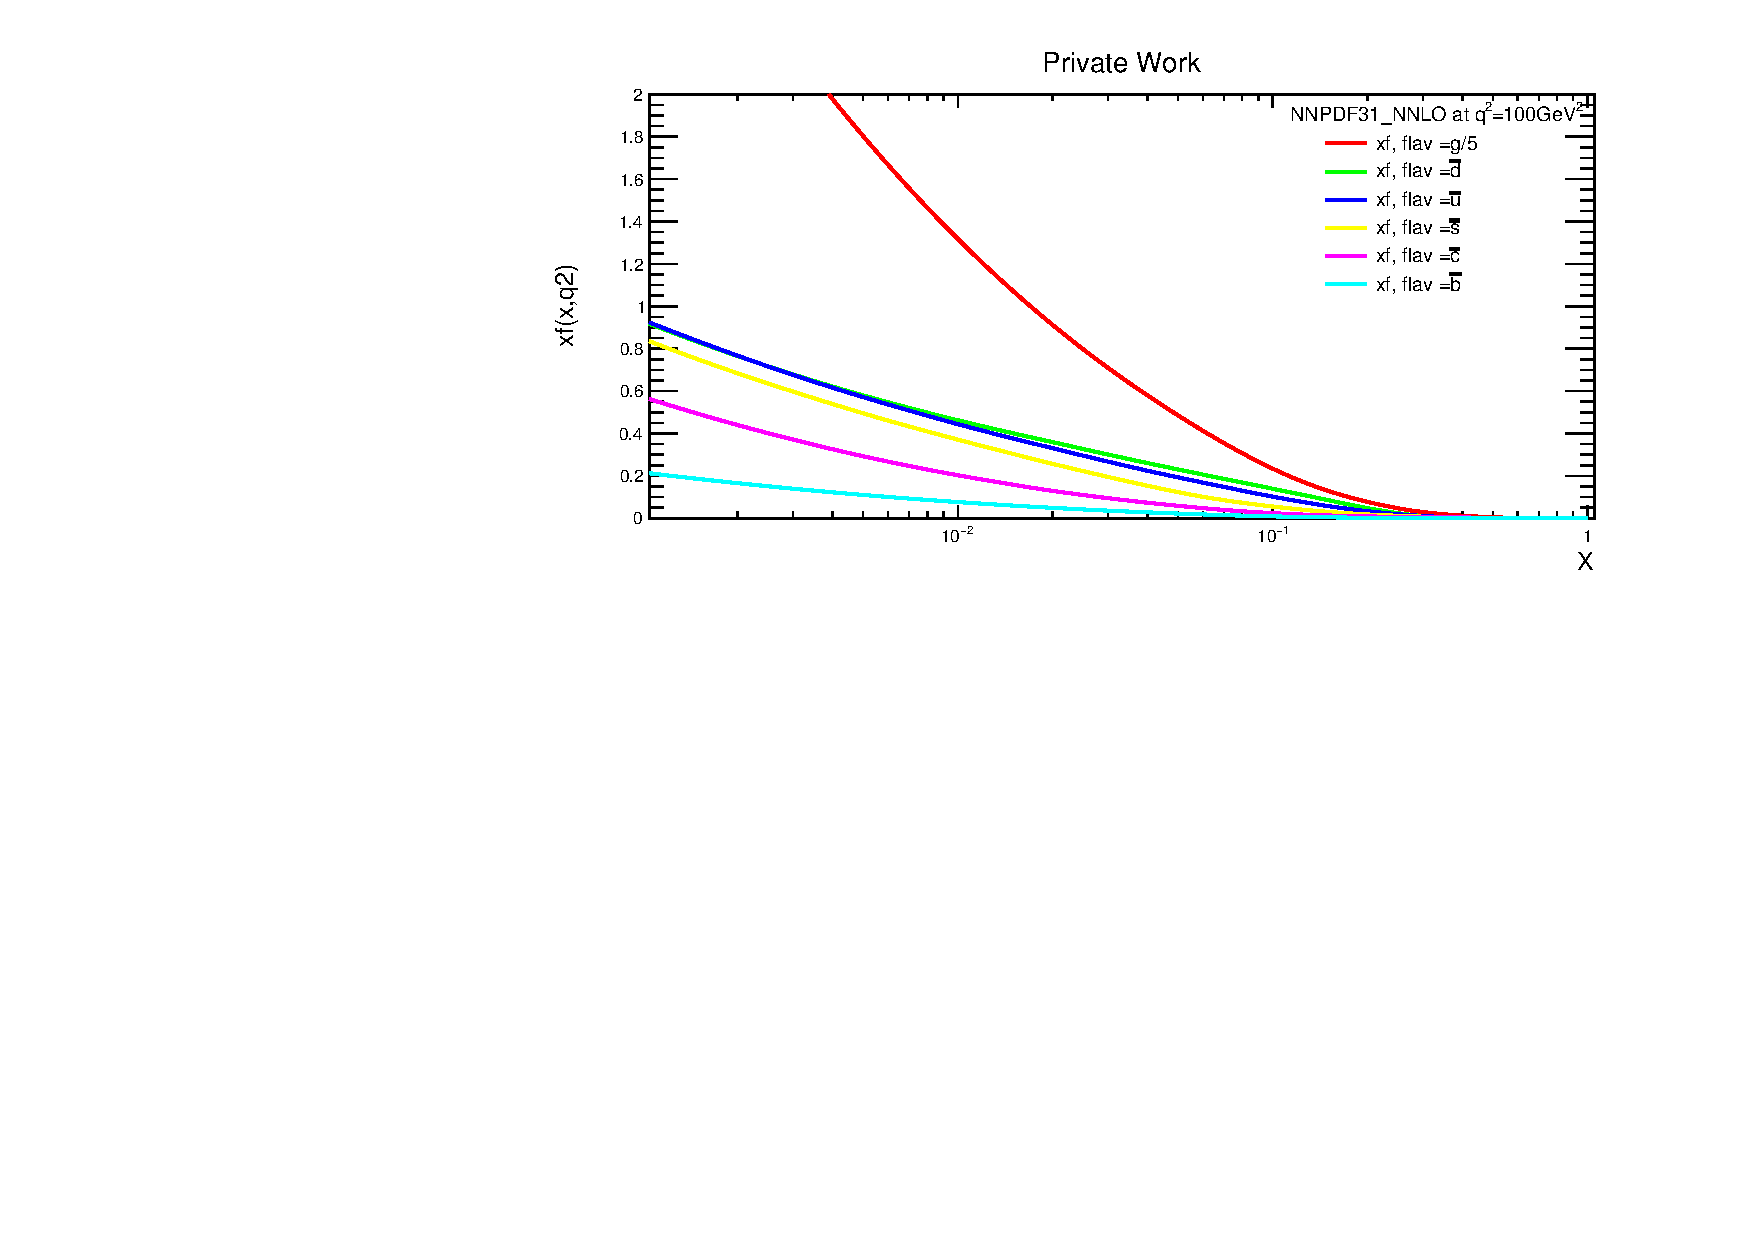
\includegraphics[height=5cm, width=\textwidth]{chapter4/barxfx100gev1.pdf}
\vspace*{-8mm}
\caption{}
\end{subfigure}
\begin{subfigure}{0.45\textwidth}
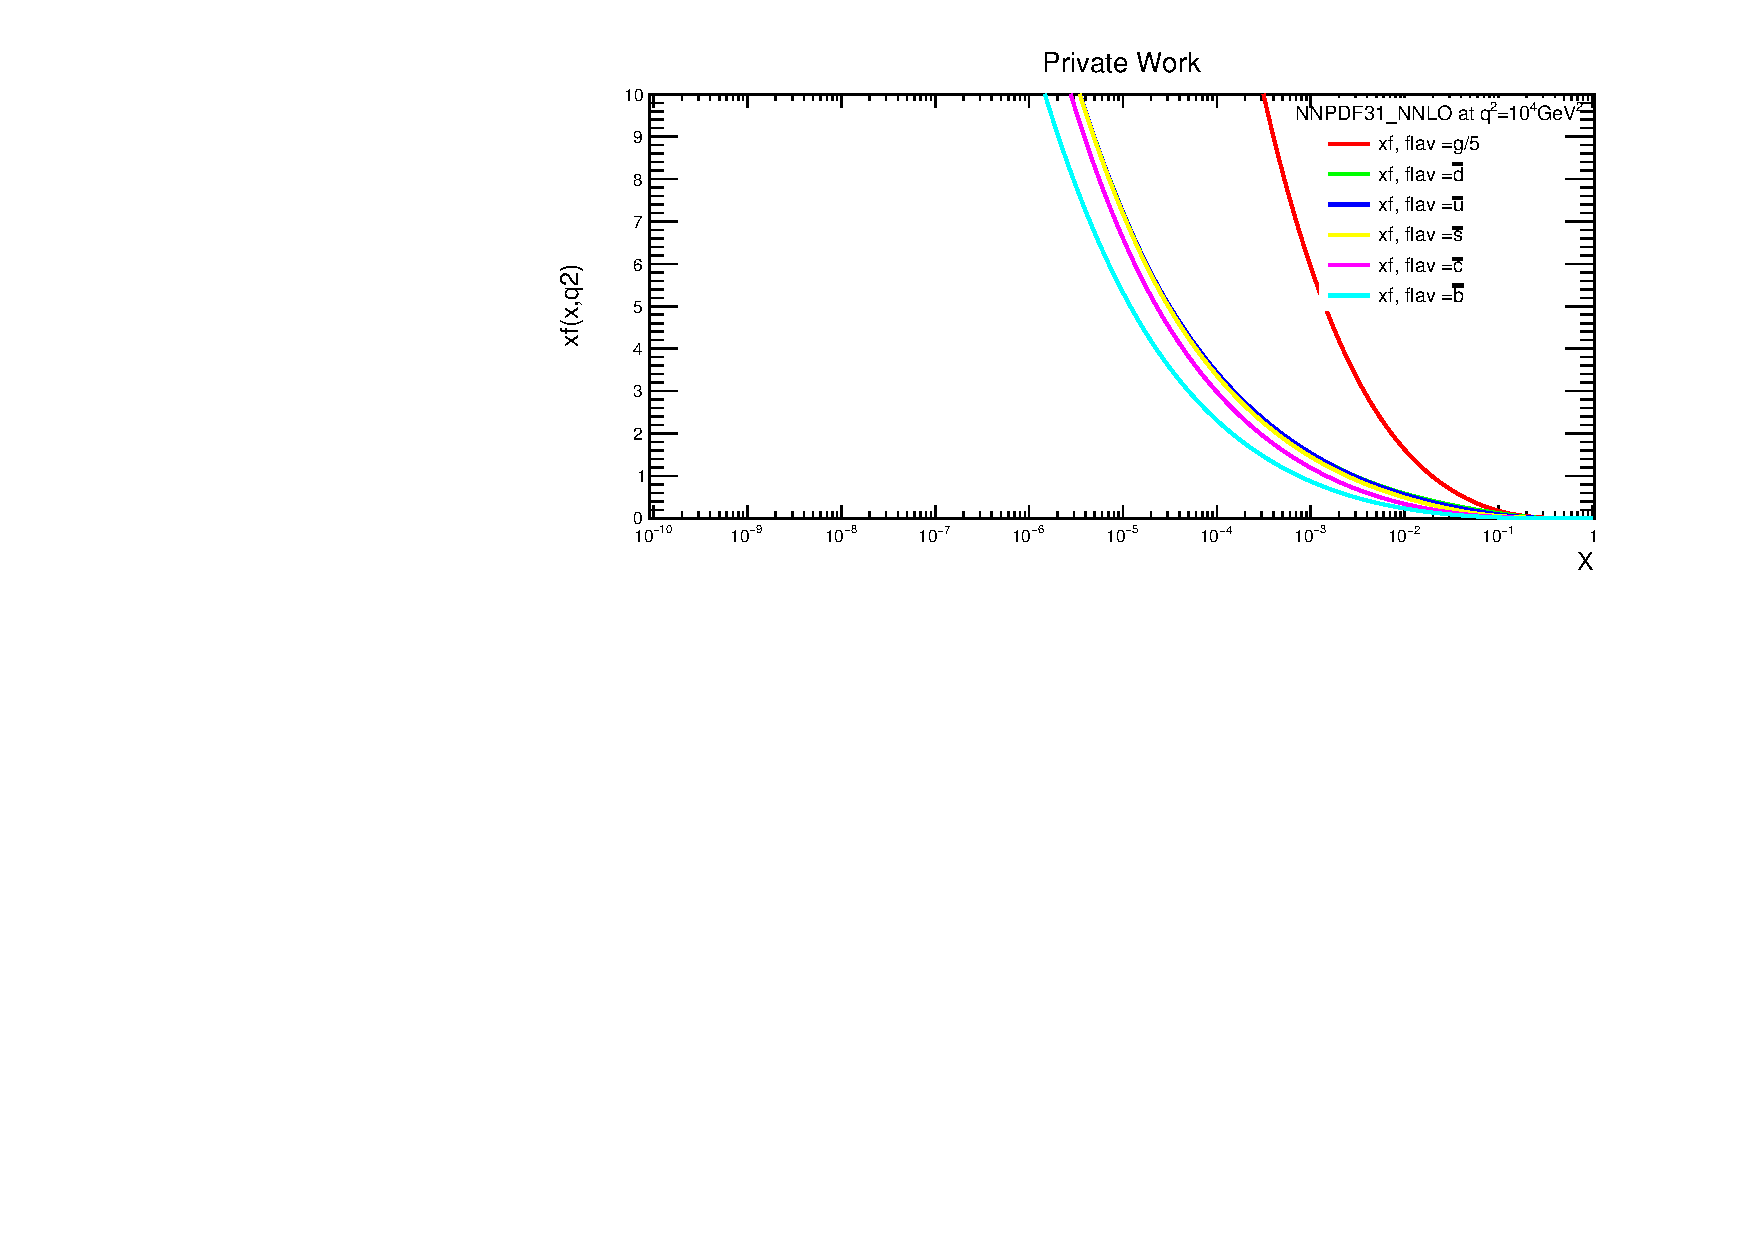
\includegraphics[height=5cm, width=\textwidth]{chapter4/barxfx10000gev.pdf}
\vspace*{-8mm}
\caption{}
\end{subfigure}
\begin{subfigure}{0.45\textwidth}
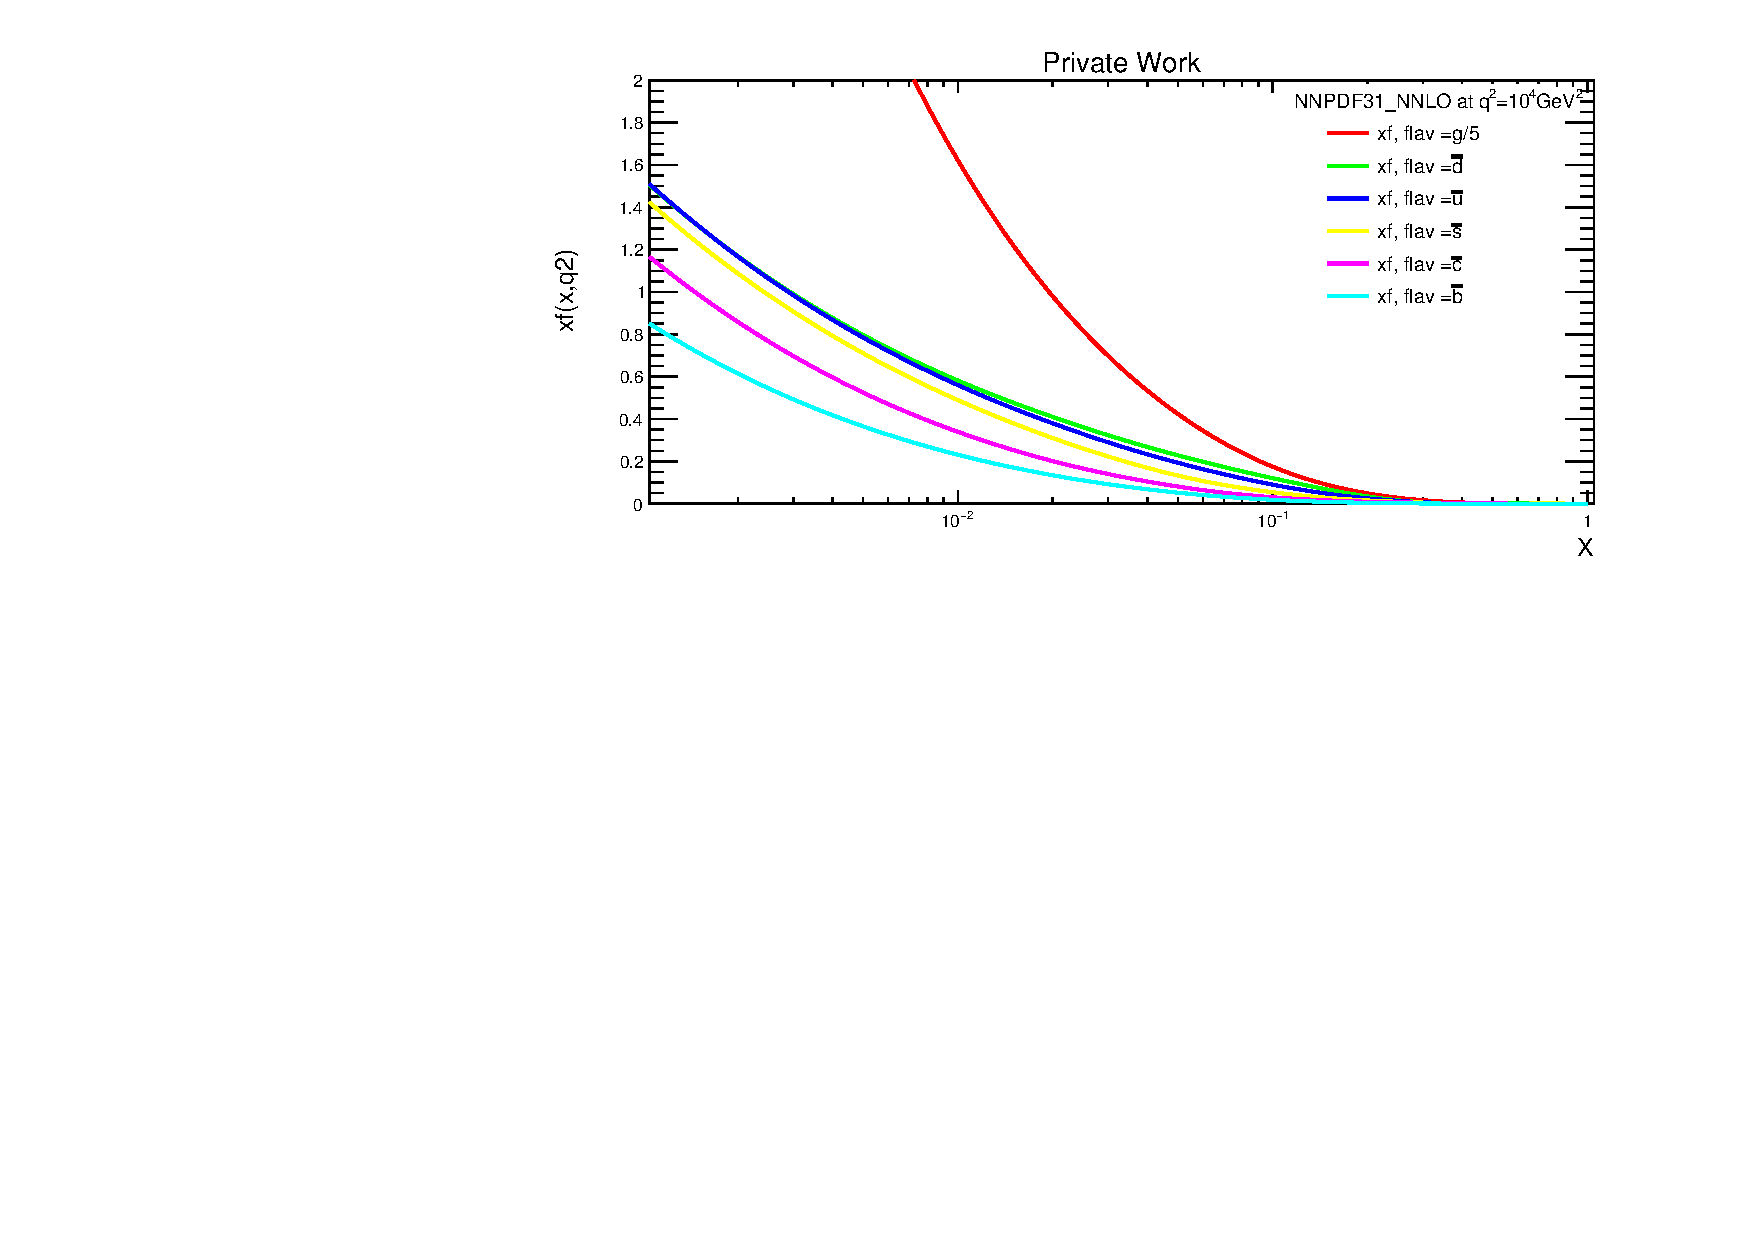
\includegraphics[height=5cm, width=\textwidth]{chapter4/barxfx10000gev1.pdf}
\vspace*{-8mm}
\caption{}
\end{subfigure}
\begin{subfigure}{0.45\textwidth}
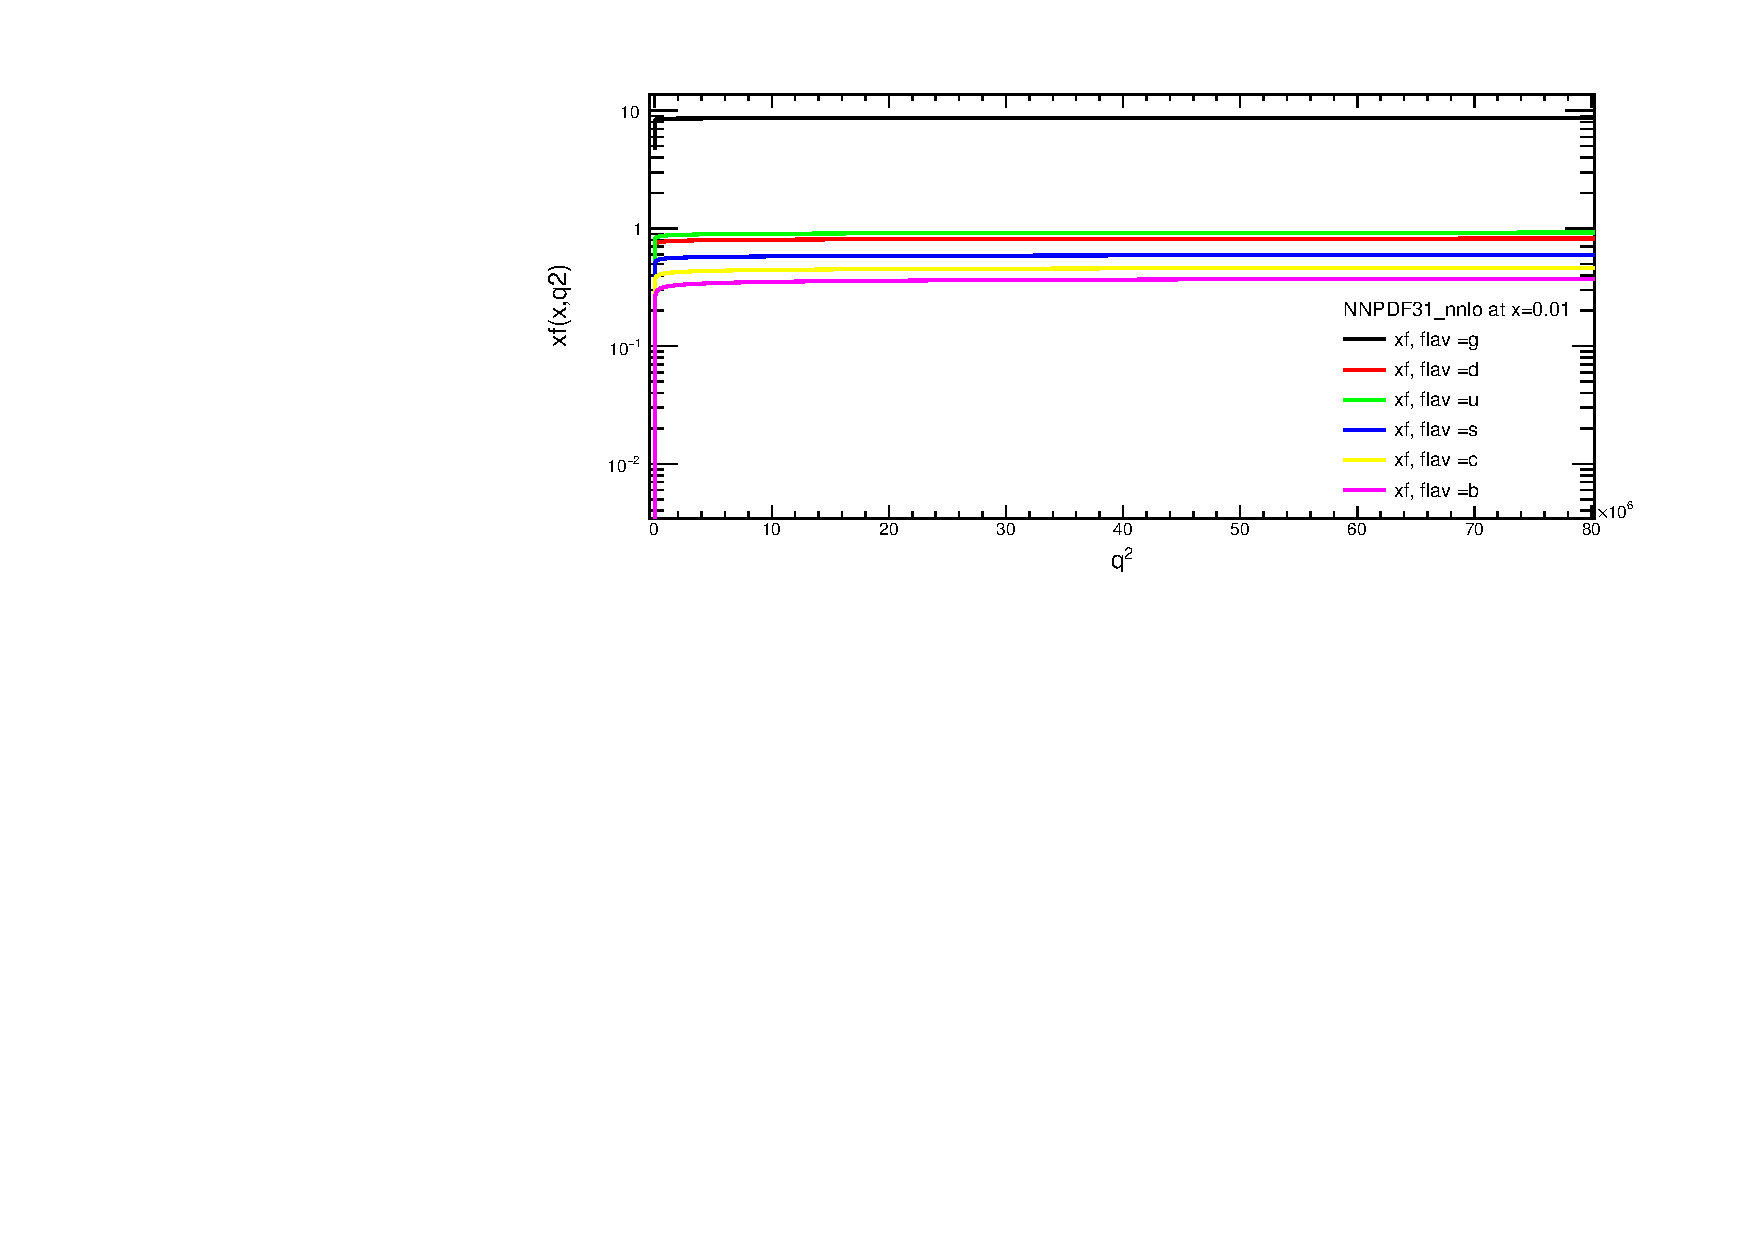
\includegraphics[height=5cm, width=\textwidth]{chapter4/qfxplot0.01.pdf}
\vspace*{-8mm}
\caption{}
\end{subfigure}
\begin{subfigure}{0.45\textwidth}
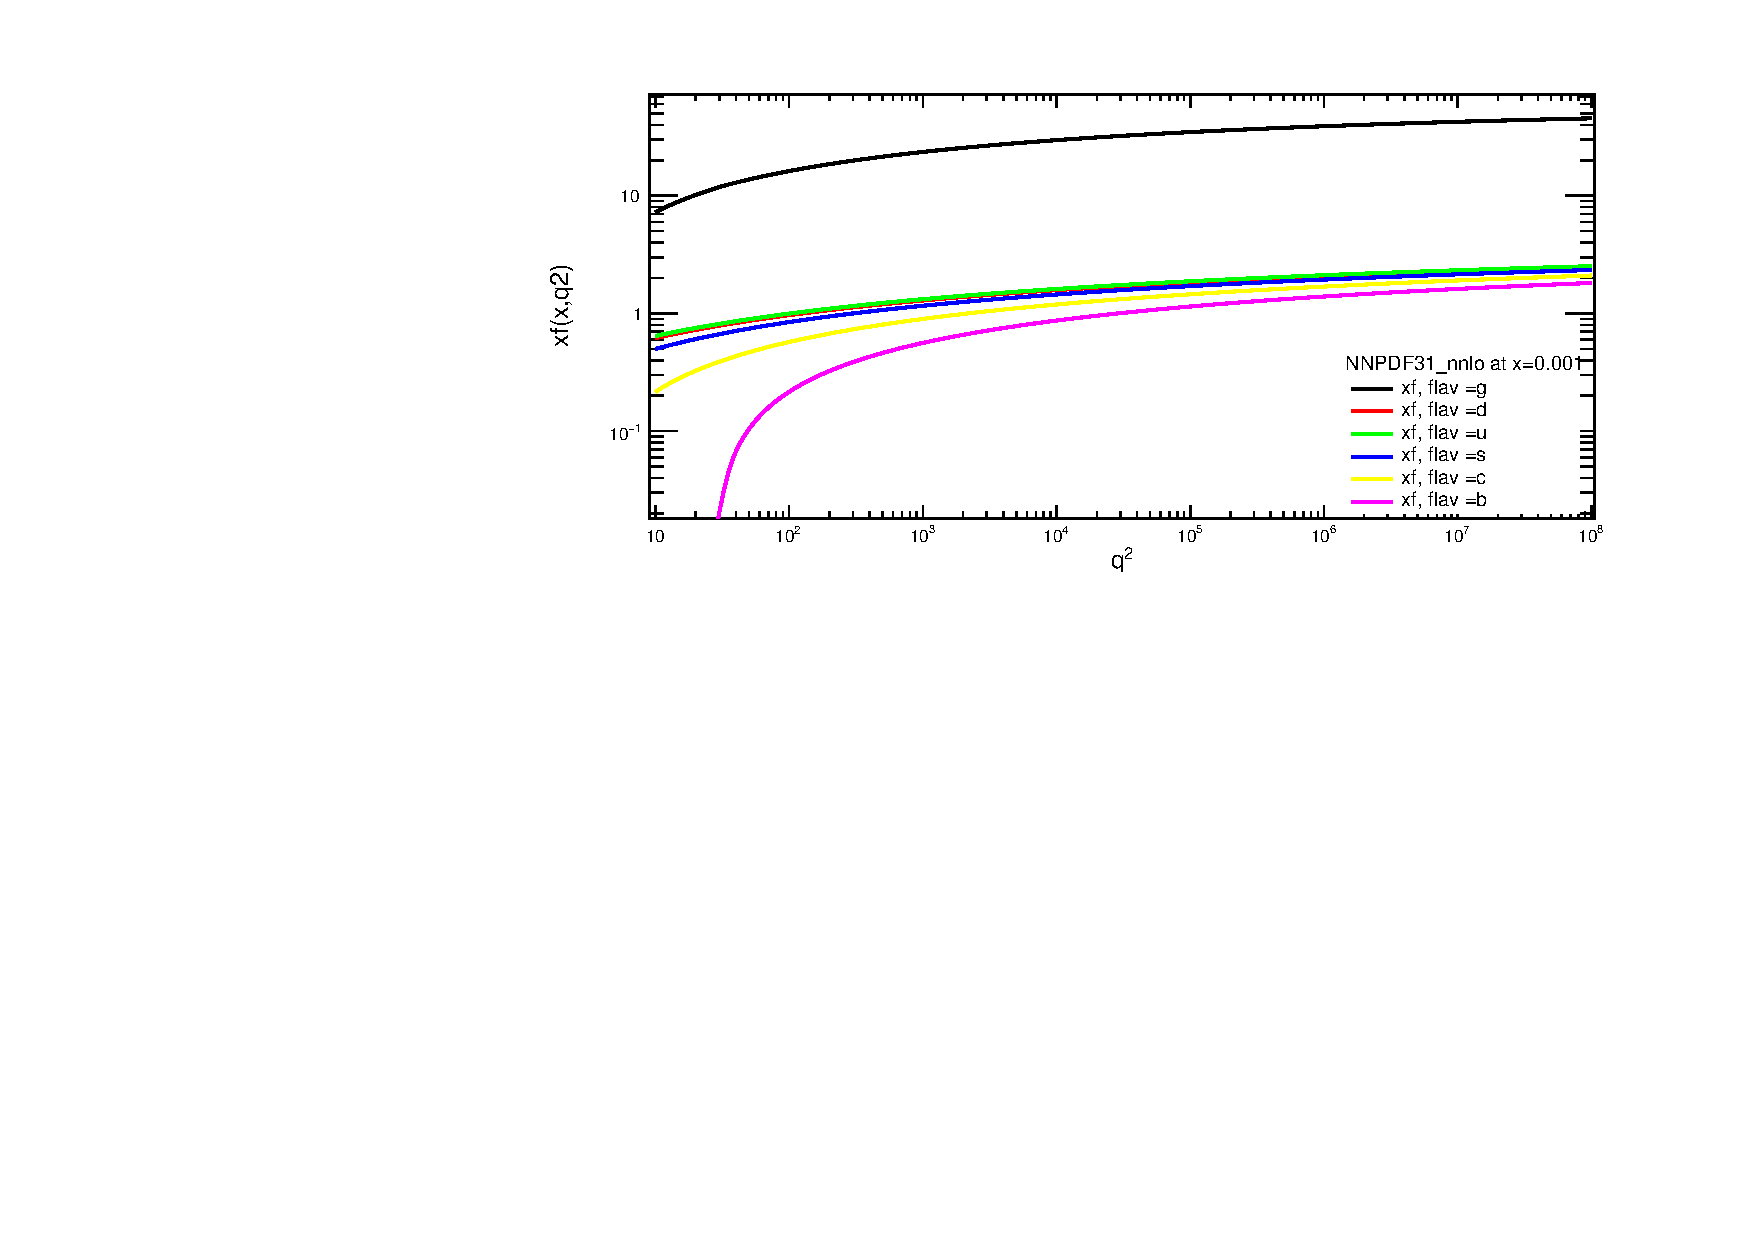
\includegraphics[height=5cm, width=\textwidth]{chapter4/qfxplot0.001.pdf}
\vspace*{-8mm}
\caption{}
\end{subfigure}
\caption{The NNPDF3.1-NNLO PDFs as a function of $x$ for the gluon~(g), down~(d),~up(u), strange~(s), charm~(c) and bottom~(b) anti-quarks.  (a), (b): for $Q^{2}= 10GeV^{2}$, (c), (d): for $Q^{2}=100GeV^{2}$ and (e), (f): for $Q^{2}=10000GeV^{2}$, (g), (h):PDF function of quarks as a function of $q$. The gluon PDFs are scaled down by a factor of 5.} 
\label{nnpdf_nnlo1}
\end{figure}  


\section{Results}
\subsection{Measurements vs Predictions}
The comparison of the measurement of the inclusive production cross section times leptonic branching ratios of $W$ and $Z$ bosons with the theoretical predictions is made. The cross sections are measured with both CMS and ATLAS data at $13TeV$ with $\mathcal{L}_{int} = 81~pb^{-1}$ in proton-proton collision. The maximum instantaneous luminosity measured was $L = 1.7\times10^{33}~cm^{-1}s^{-1}$.\\
The theoretical prediction for $W$, $Z$, $W^{+}$ and $W^{-}$ production cross section times BR($W\rightarrow l\nu,~Z\rightarrow ll$) are predicted for both $13~TeV$ and $14~TeV$ center of mass energy and we also made a comparison with the previous results obtained at $7~TeV$ and $8~TeV$. The Theoretical predictions are made using NNPDF3.1 PDF at LO, NLO and NNLO and various uncertainties in predictions are also measured.\\
The ratios of the cross sections~i.e $R_{W^{\pm}~=~\frac{\sigma_{W^{+}}}{\sigma_{W^{-}}}}$ and $R_{WZ}~=~\frac{\sigma_{W^{\pm}}}{\sigma_{Z}}$ measured at $8~TeV$ and $13~TeV$ are compared and prediction for $14~TeV$ is made.\\

\subsubsection{8~TeV}
The Tables \ref{8tev_tab} and \ref{8tev_tab1} shows the measured cross sections of $W$ and $Z$ boson times branching fraction $\sigma\times~BR(W\rightarrow l\nu,~Z\rightarrow ll)$ and theoretically predicted cross sections. The uncertainty in the measured values are due to statistical, systematic and luminosity errors. The measured values are taken from reference~\cite{Chatrchyan_2014}. 
\begin{table}[H]
\caption{The measured total $\sigma^{tot}$ cross sections for leptonic decay channels~(electron, muon) of $W^{-}$, $W^{+}$, $W^{\pm}$ and $Z$-bosons at CMS with $8~TeV, 18.2~pb^{-1}$, and predicted total cross section at $8~TeV$. The uncertainties in measurement due to statistical, systematic and luminosity error. The NNPDF3.1-NNLO PDF is used for the predictions.}
\centering
\begin{tabular}{|l|p{6cm}|p{6cm}| }
\hline
channel&\bf Measured Cross section~[nb]&\bf Predicted Cross section~[nb]\newline (value$\pm$PDF)\\
\hline
\hline
$W^{-}$&5.09~$\pm$~0.02~$\pm$~0.11~$\pm$~0.18&5.21~$\pm$~0.04\\
$W^{+}$&7.11~$\pm$0.03~$\pm$~0.14~$\pm$~0.13&7.39~$\pm$~0.06\\
$W^{\pm}$&12.21~$\pm$~0.02~$\pm$~0.55~$\pm$~0.43&12.60~$\pm$~0.08\\
\hline
\hline
$Z$&1.15~$\pm$~0.01~$\pm$~0.02~$\pm$~0.03&1.26~$\pm$~0.01\\
\hline

\end{tabular}
\label{8tev_tab}
\end{table}

\begin{table}[H]
\caption{Measured values with statistical and systematic errors and predicted Ratios $W^{+}/W^{-}$ and $W^{\pm}/Z$ at 8~TeV. For prediction NNPDF3.1-NNLO PDF is used.}
\centering
\begin{tabular}{|l|p{6cm}|p{6cm}|}
\hline
Channel&\bf Measured Ratio&\bf Predicted Ratio\newline(value$\pm$PDF)\\
\hline
\hline
$W^{+}/W^{-}$&1.40~$\pm$~0.01~$\pm$~0.02&1.42~$\pm$~0.01~\\
$W^{\pm}/Z$&10.63~$\pm$~0.11~$\pm$~0.25&10.00~$\pm$~0.11\\
\hline
\end{tabular}
\label{8tev_tab1}
\end{table}

\subsubsection{13~TeV}
Tables \ref{13_tab} and \ref{13_tab1} show the measured cross section of vector bosons and predictions at $13~TeV$ with NNPDF3.1-NNLO PDF. 
\begin{table}[H]
\caption{The measured~\cite{Aad_2016}~\cite{CMS:2015ois} total $\sigma^{tot}$ cross sections with statistical, systematic and luminosity error for the electron channel of $W^{-}$, $W^{+}$, $W^{\pm}$ and $Z-$boson, and predicted total cross section at 13~TeV. The NNPDF3.1-NNLO PDF is used for the predictions.}
\centering
\begin{tabular}{|l|p{6cm}|p{6cm}| }
\hline
channel&\bf Measured Cross section~[nb] &\bf Predicted Cross section~[nb]\newline (value$\pm$PDF$\pm\alpha_{S}$ $\pm$PDF+$\alpha_{S}$)\\
\hline
\hline
$W^{-}$&8.79~$\pm$~0.02~$\pm$~0.24~$\pm$~0.18&8.95~$\pm$~0.07~$\pm$~0.07~$\pm$~0.09\\
$W^{+}$&11.83~$\pm$~0.02~$\pm$~0.34~$\pm$~0.25&12.03~$\pm$~0.11~$\pm$~0.09~$\pm$~0.14\\
$W^{\pm}$&20.64~$\pm$~0.02~$\pm$~0.55~$\pm$~0.43&20.98~$\pm$~0.13$\pm$~0.16~$\pm$~0.20\\
\hline
\hline
$Z$&1.98~$\pm$~0.007~$\pm$~0.04~$\pm$~0.04&2.14~$\pm$~0.02~$\pm$~0.01~$\pm$~0.02\\
\hline
\end{tabular}
\label{13_tab}
\end{table}
 
\begin{table}[H]
\centering
\caption{Measured ratio with statistical ans systematic errors and predicted Ratios $W^{+}/W^{-}$ and $W^{\pm}/Z$ at 13~TeV. For prediction NNPDF3.1-NNLO PDF is used. The measured values are taken from reference~\cite{Aad_2016}}
\begin{tabular}{|l|p{6cm}|p{6cm}|}
\hline
Channel&\bf Measured Ratio&\bf Predicted Ratio\newline(value$\pm$PDF$\pm$PDF$+\alpha_{s}$)\\
\hline
\hline
$W^{+}/W^{-}$&1.295~$\pm$~0.003~$\pm$~0.01&1.34~$\pm$~0.016~$\pm$~0.02\\
$W^{\pm}/Z$&10.31~$\pm$~0.04~$\pm$~0.20&9.8~$\pm$~0.09~$\pm$~0.13\\
\hline
\end{tabular}
\label{13_tab1}
\end{table}

\subsubsection{14~TeV}
Tables \ref{14_tab} and \ref{14_tab1} shows the predicted cross section for the vector bosons at $14~TeV$ with NNPDF3.1-NNLO PDF. 
\begin{table}[H]
\centering
\caption{Predicted total cross section of $W^{-}$, $W^{+}$, $W^{\pm}$ and $Z$ boson at $14~TeV$.The NNPDF3.1-NNLO PDF is used for the predictions.}
\begin{tabular}{|l|p{6cm}|p{6cm}| }
\hline
channel&\bf Cross section~[nb] \newline (To be measured) &\bf Predicted Cross section~[nb]\newline (value$\pm$PDF$\pm\alpha_{S}$ $\pm$PDF+$\alpha_{S}$)\\
\hline
\hline
$W^{-}$&---------&9.70~$\pm$~0.08~$\pm$~0.14~$\pm$~0.16\\
$W^{+}$&---------&12.94~$\pm$~0.12~$\pm$~0.12~$\pm$~0.23\\
$W^{\pm}$&---------&22.63~$\pm$~0.15~$\pm$~0.17~$\pm$~0.22\\
\hline
\hline
$Z$&---------&2.316~$\pm$~0.02~$\pm$~0.02~$\pm$~0.02\\
\hline
\end{tabular}
\label{14_tab}
\end{table}

\begin{table}[H]
\centering
\caption{Predicted Ratios $W^{+}/W^{-}$ and $W^{\pm}/Z$ at $14TeV$. For prediction NNPDF3.1-NNLO PDF is used.} 
\begin{tabular}{|l|p{6cm}|p{6cm}|}
\hline
Channel&\bf Cross section ratios \newline (To be measured) &\bf Predicted ratios\newline(value$\pm$PDF$\pm$PDF$+\alpha_{s}$)\\
\hline
\hline
$W^{+}/W^{-}$&---------&1.33~$\pm~0.01~\pm~0.03$\\
$W^{\pm}/Z$&----------&9.77~$\pm~0.09~\pm~0.21$\\
\hline
\end{tabular}
\label{14_tab1}
\end{table}


\section{Theoretical Predictions and Uncertainties in Cross Section of $W$ and $Z$ Bosons.}
The predicted increase in measurement of cross section of $W$ and $Z$ bosons with the center of mass energy can be seen in Fig.~\ref{pre_inc}. The cross section value at $14~TeV$ yet to be measured. The Predicted cross section of $W$, $Z$, $W^{+}$ and $W^{-}$ in $pb$ are plotted with various uncertainties in predictions. These uncertainties are determined at both $68\%$ and $90\%$ C.L. The errors are determined with both Monte-Carlo replicas and Hessian error eigen vector method. The variation in predictions with the variation in QCD scale are also determined. Results are shown in Fig.~\ref{NLO_WZ} Fig.~\ref{13tev1},~Fig.~\ref{13tev2},~Fig.~\ref{13tev3} and Fig.~\ref{13tev4} 
\begin{figure}[H]
    \centering
    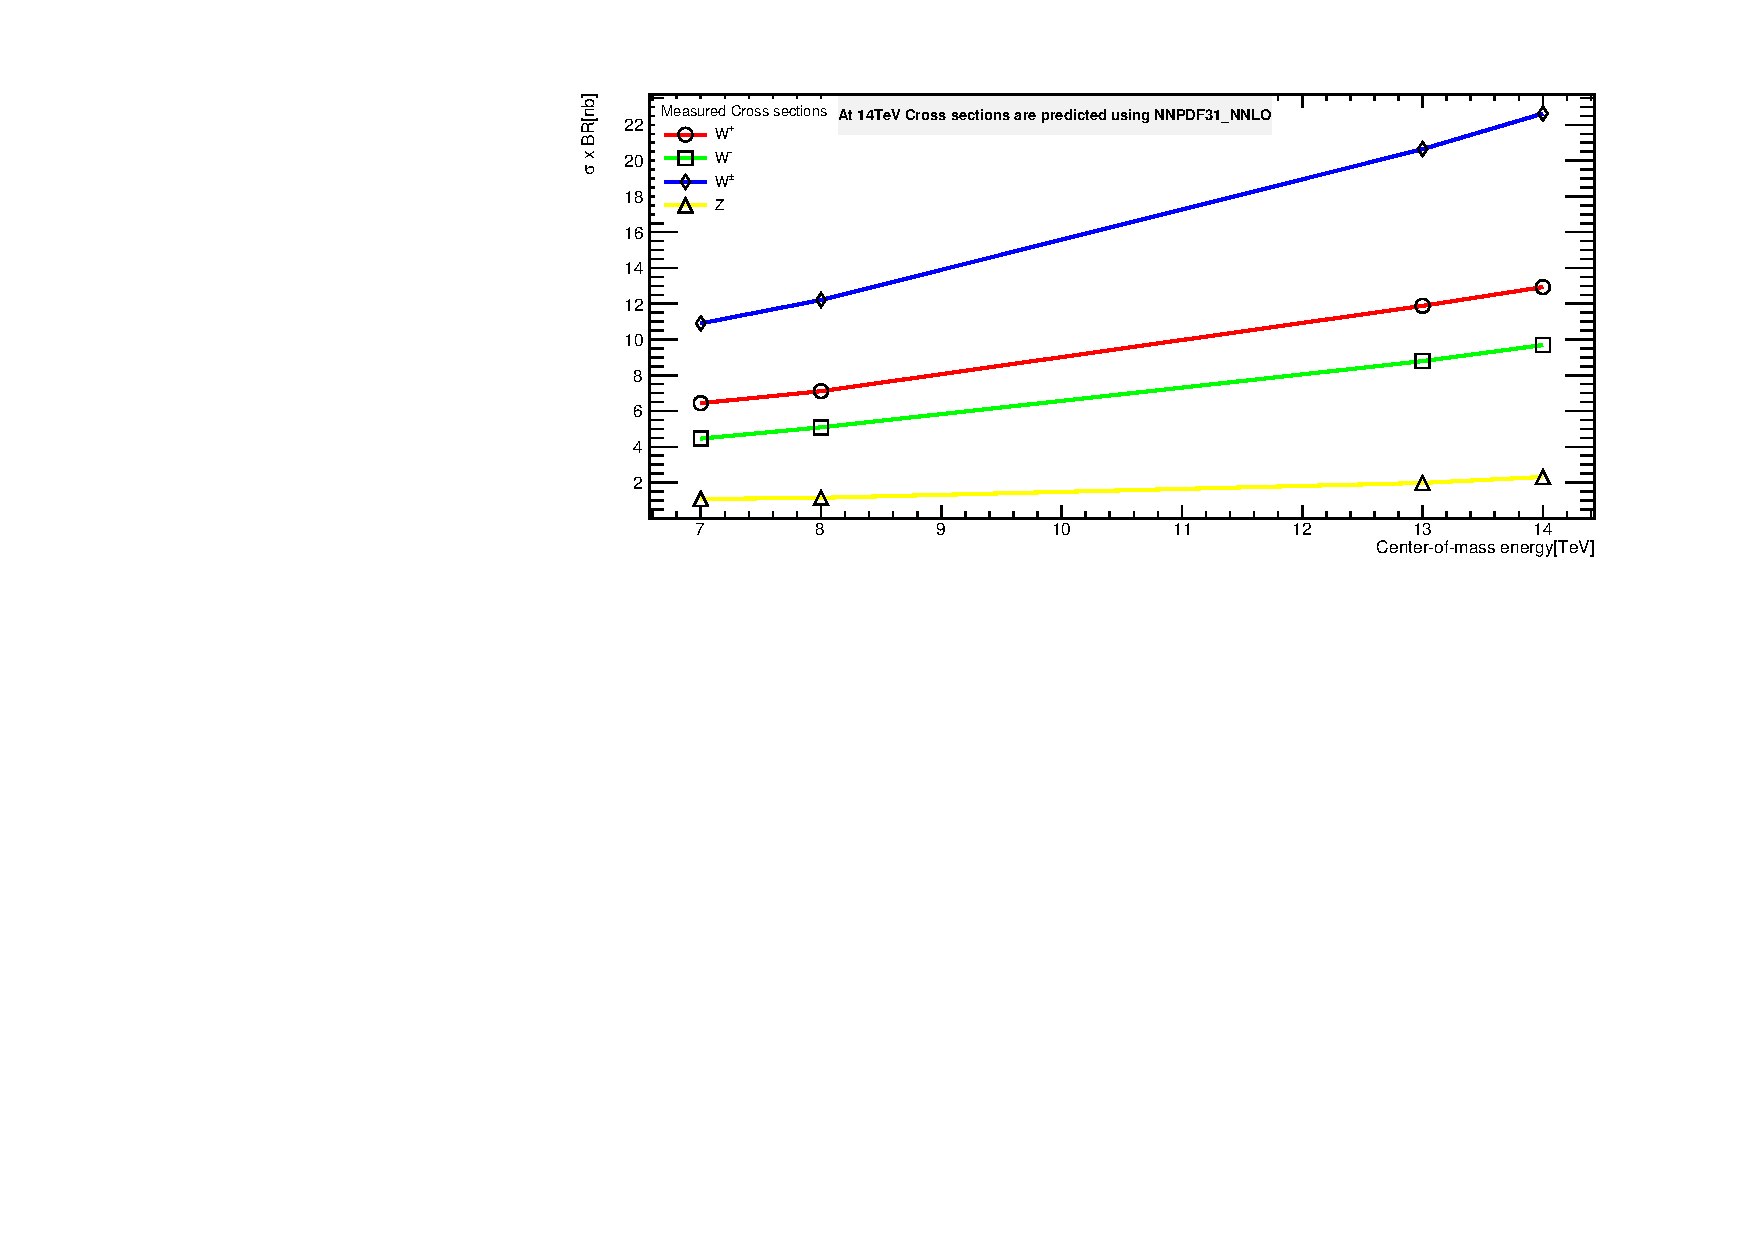
\includegraphics[scale=0.7]{chapter4/Com_var.pdf}
    \caption{Figure~\ref{pre_inc} shows measured cross section of ($W^{+},W^{-},Z$ and $W^{\pm}$) with the variation of center of mass energy and at $14~TeV$ value of cross section is predicted at NNLO.}
    \label{pre_inc}
\end{figure}


\begin{figure}[H]
\centering
\begin{subfigure}{\textwidth}
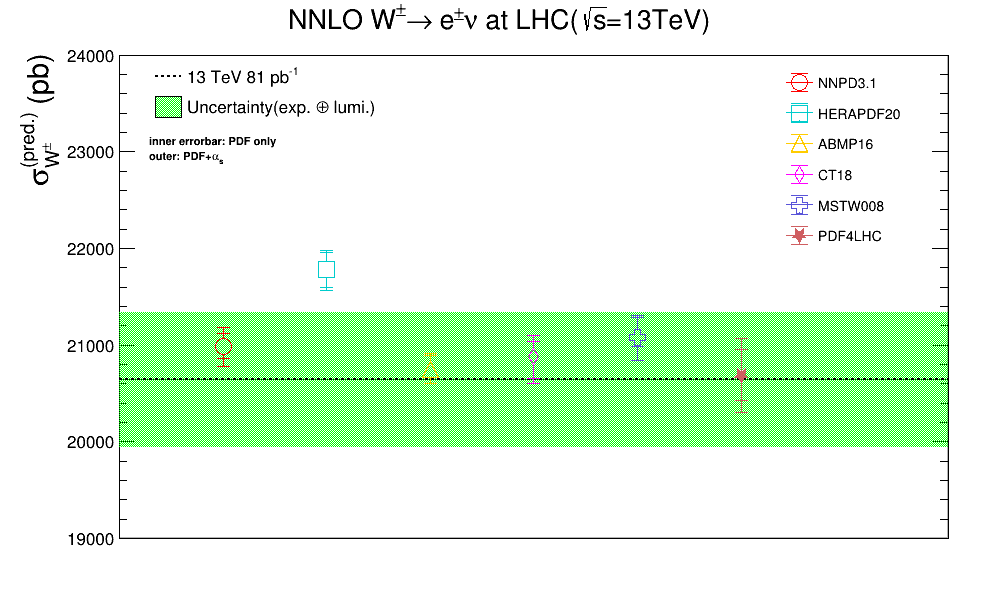
\includegraphics[width=0.8\textwidth, height=0.4\textheight]{chapter4/W.png}
\vspace*{-4mm}
\caption{}
\label{WCSNNLO}
\end{subfigure}
\caption{\ref{WCSNNLO} showing the predicted cross section of $W$ boson at 13~TeV NNLO using various Parton Distribution Function. The measured values are taken from~\cite{Aad_2016}}
\label{WCSNNLO1}
\end{figure}

\begin{figure}[H]
\centering
\begin{subfigure}{\textwidth}
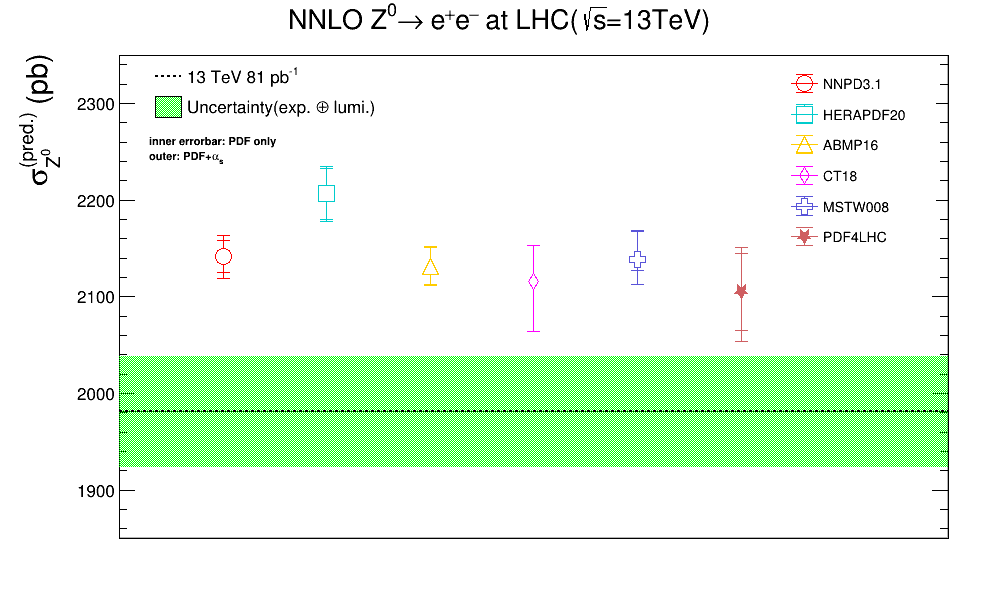
\includegraphics[width=0.8\textwidth, height=0.4\textheight]{chapter4/ZCs.png}
\vspace*{-6mm}
\caption{}
\label{ZCSNNLO}
\end{subfigure}
\caption{\ref{ZCSNNLO} showing the predicted cross section of $Z$ boson at 13~TeV NNLO using various Parton Distribution Function. The measured values are taken from~\cite{Aad_2016} }
\label{WZCS}
\end{figure}

\begin{figure}[H]
\centering
\begin{subfigure}{\textwidth}
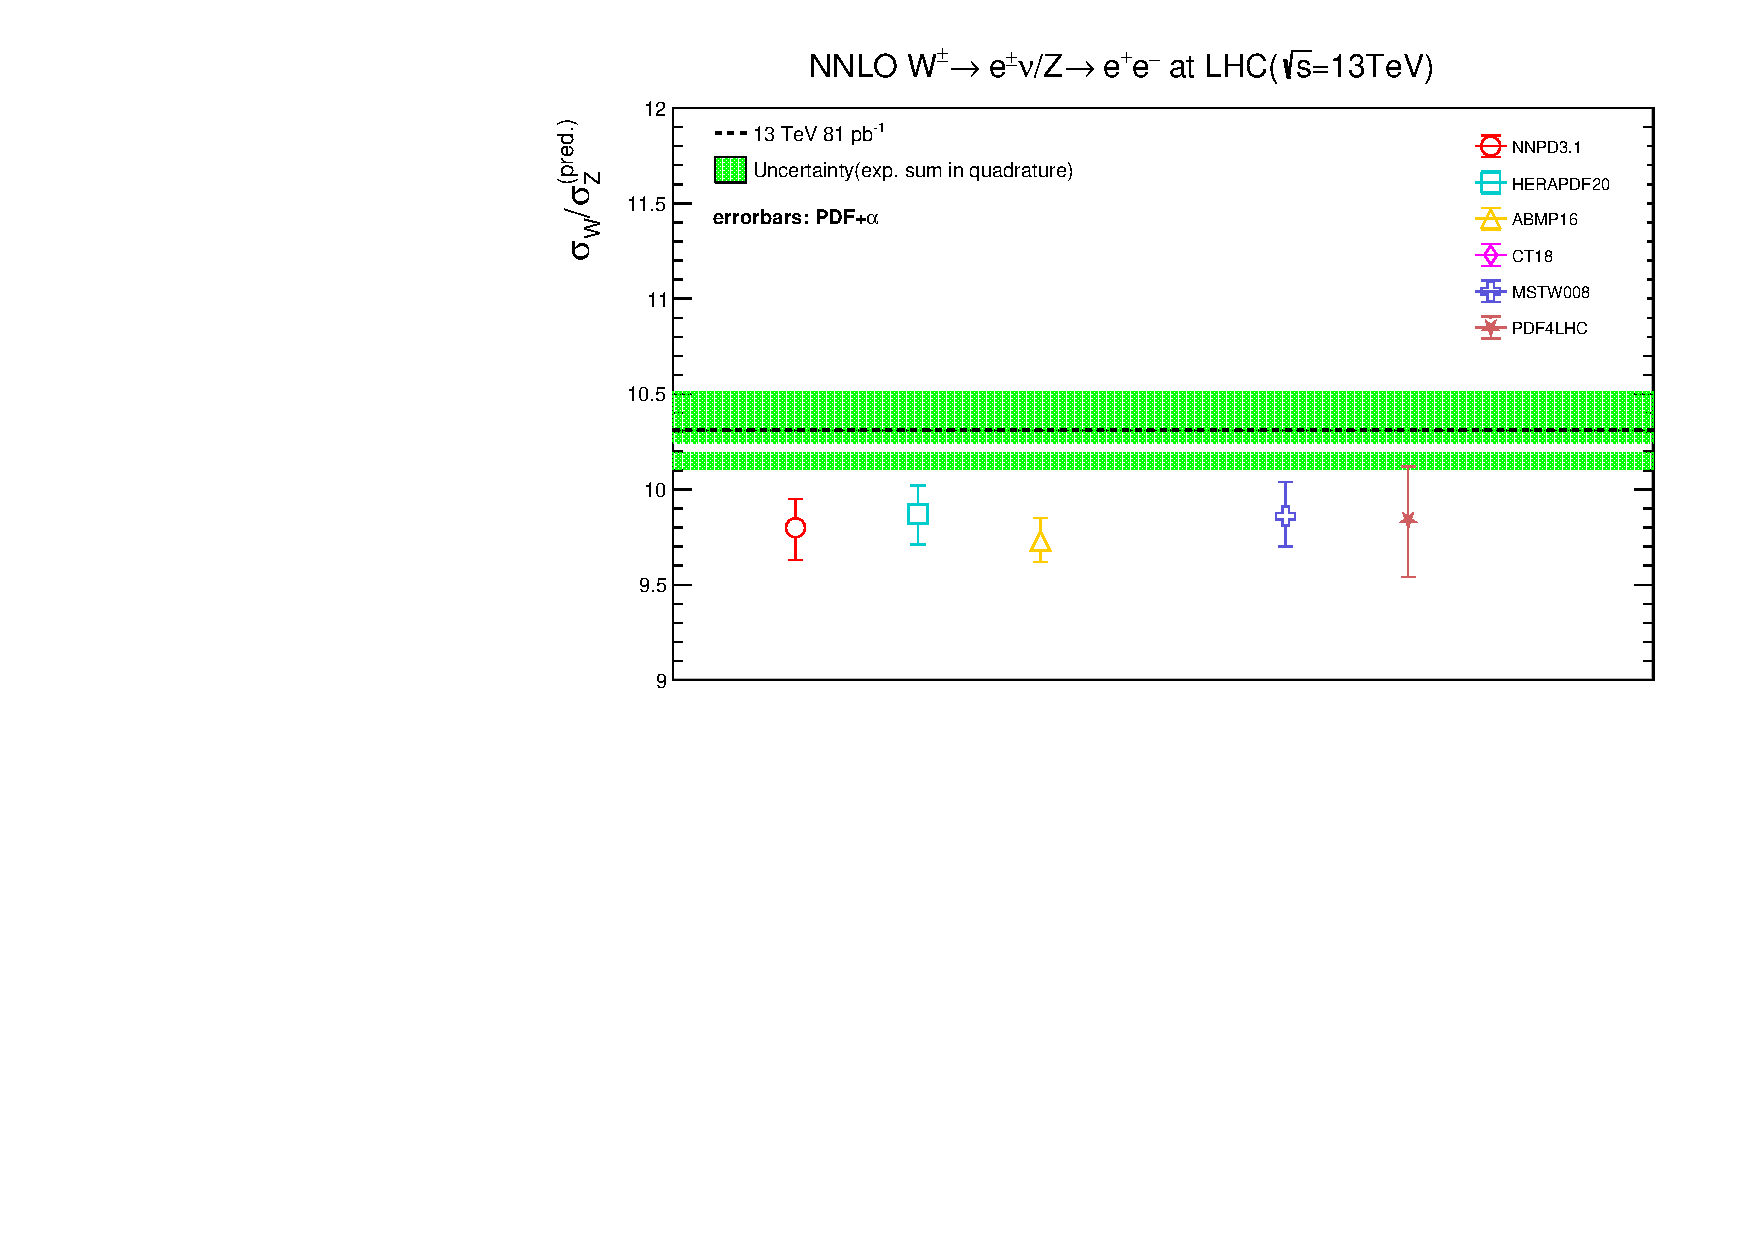
\includegraphics[scale=0.7]{chapter4/Ratiowz.pdf}
\vspace*{-6mm}
\caption{}
\label{Ratiowz}
\end{subfigure}
\caption{\ref{Ratiowz} showing the predicted cross section Ratio of $W$ and $Z$ boson at 13~TeV NNLO using various Parton Distribution Functions. The measured values are taken from~\cite{Aad_2016} }
\label{RWZ}
\end{figure}

\begin{figure}[H]
\centering
\begin{subfigure}{\textwidth}
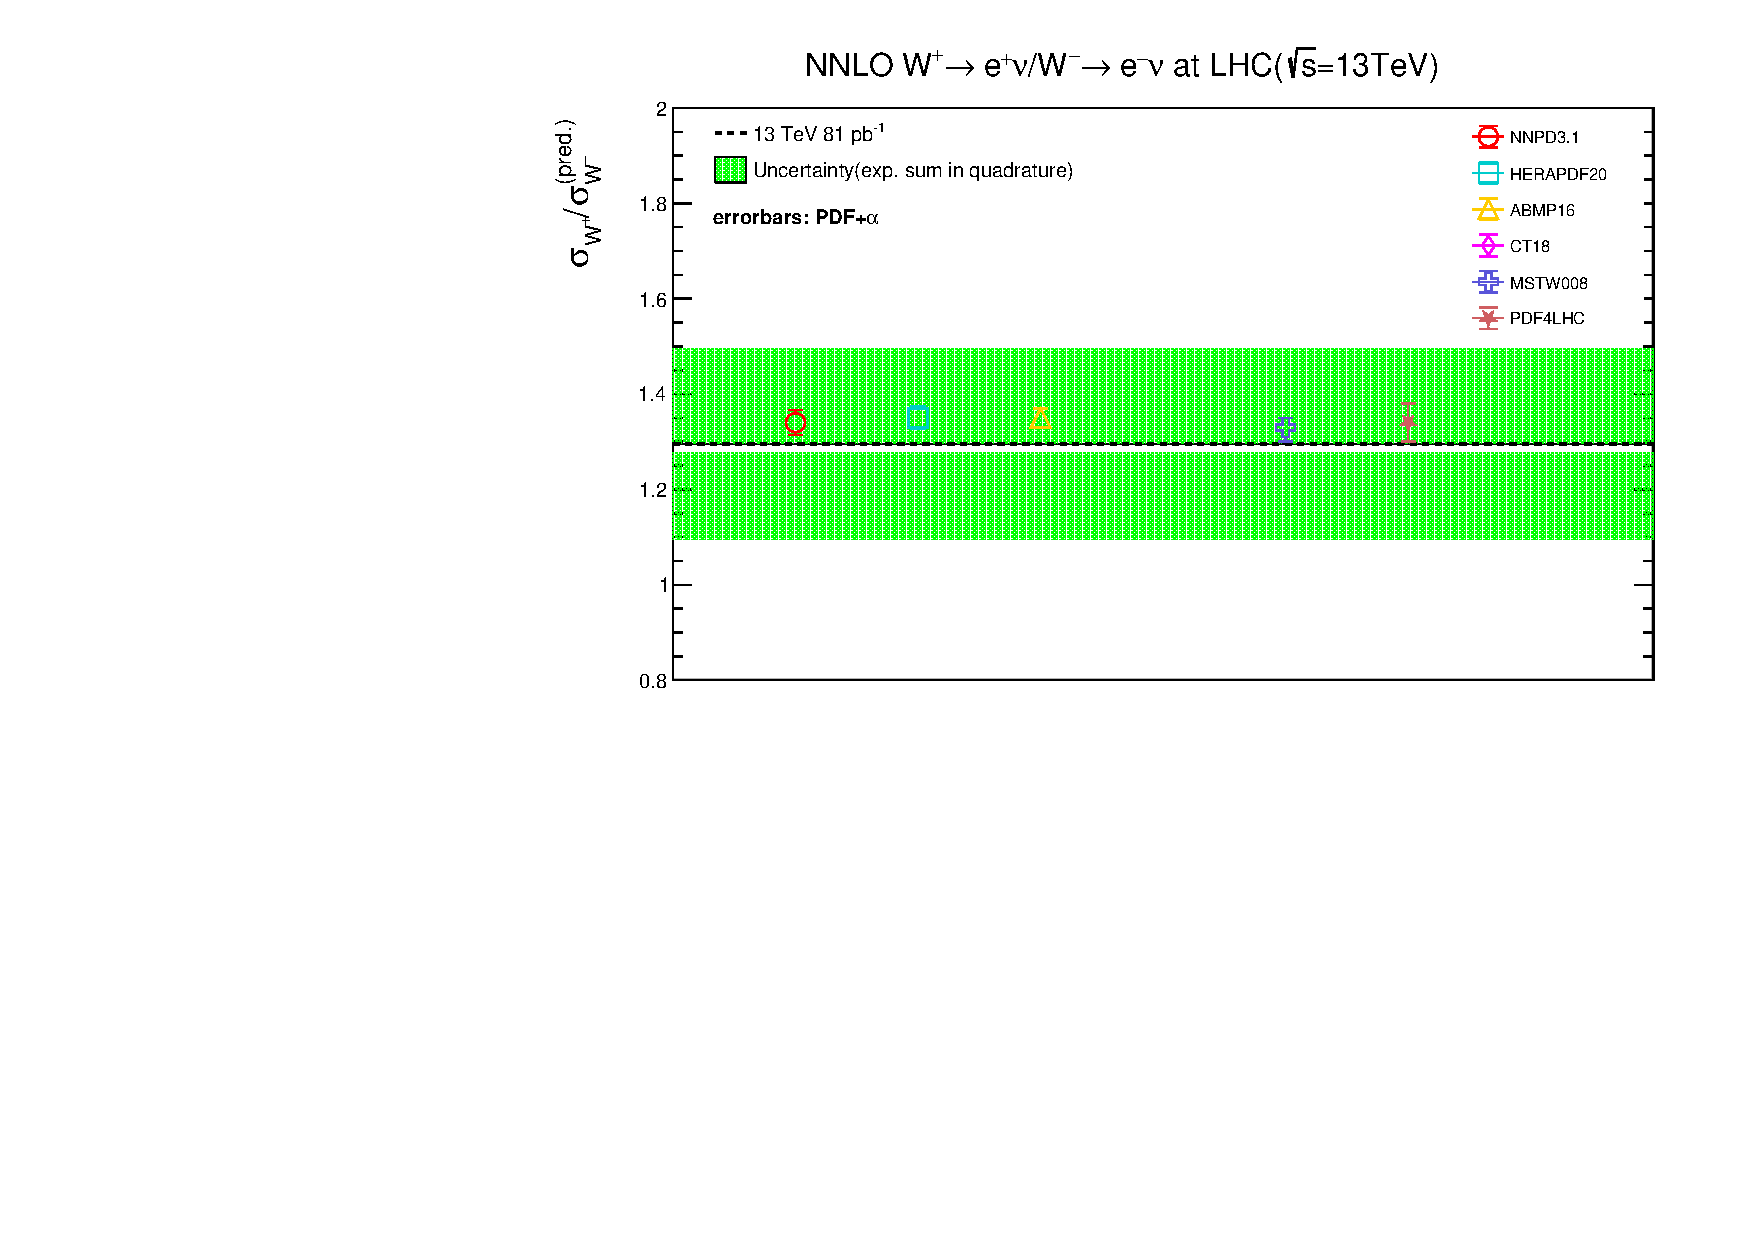
\includegraphics[scale=0.7]{chapter4/Ratioww13.pdf}
\vspace*{-6mm}
\caption{}
\label{Ratioww}
\end{subfigure}
\caption{\ref{Ratioww} showing the predicted cross section Ratio of $W^{+}$ and $W^{-}$ boson at 13~TeV NNLO using various Parton Distribution Functions. The measured values are taken from~\cite{Aad_2016} }
\label{RWw}
\end{figure}

\begin{figure}[H]
\centering
\begin{subfigure}{0.49\textwidth}
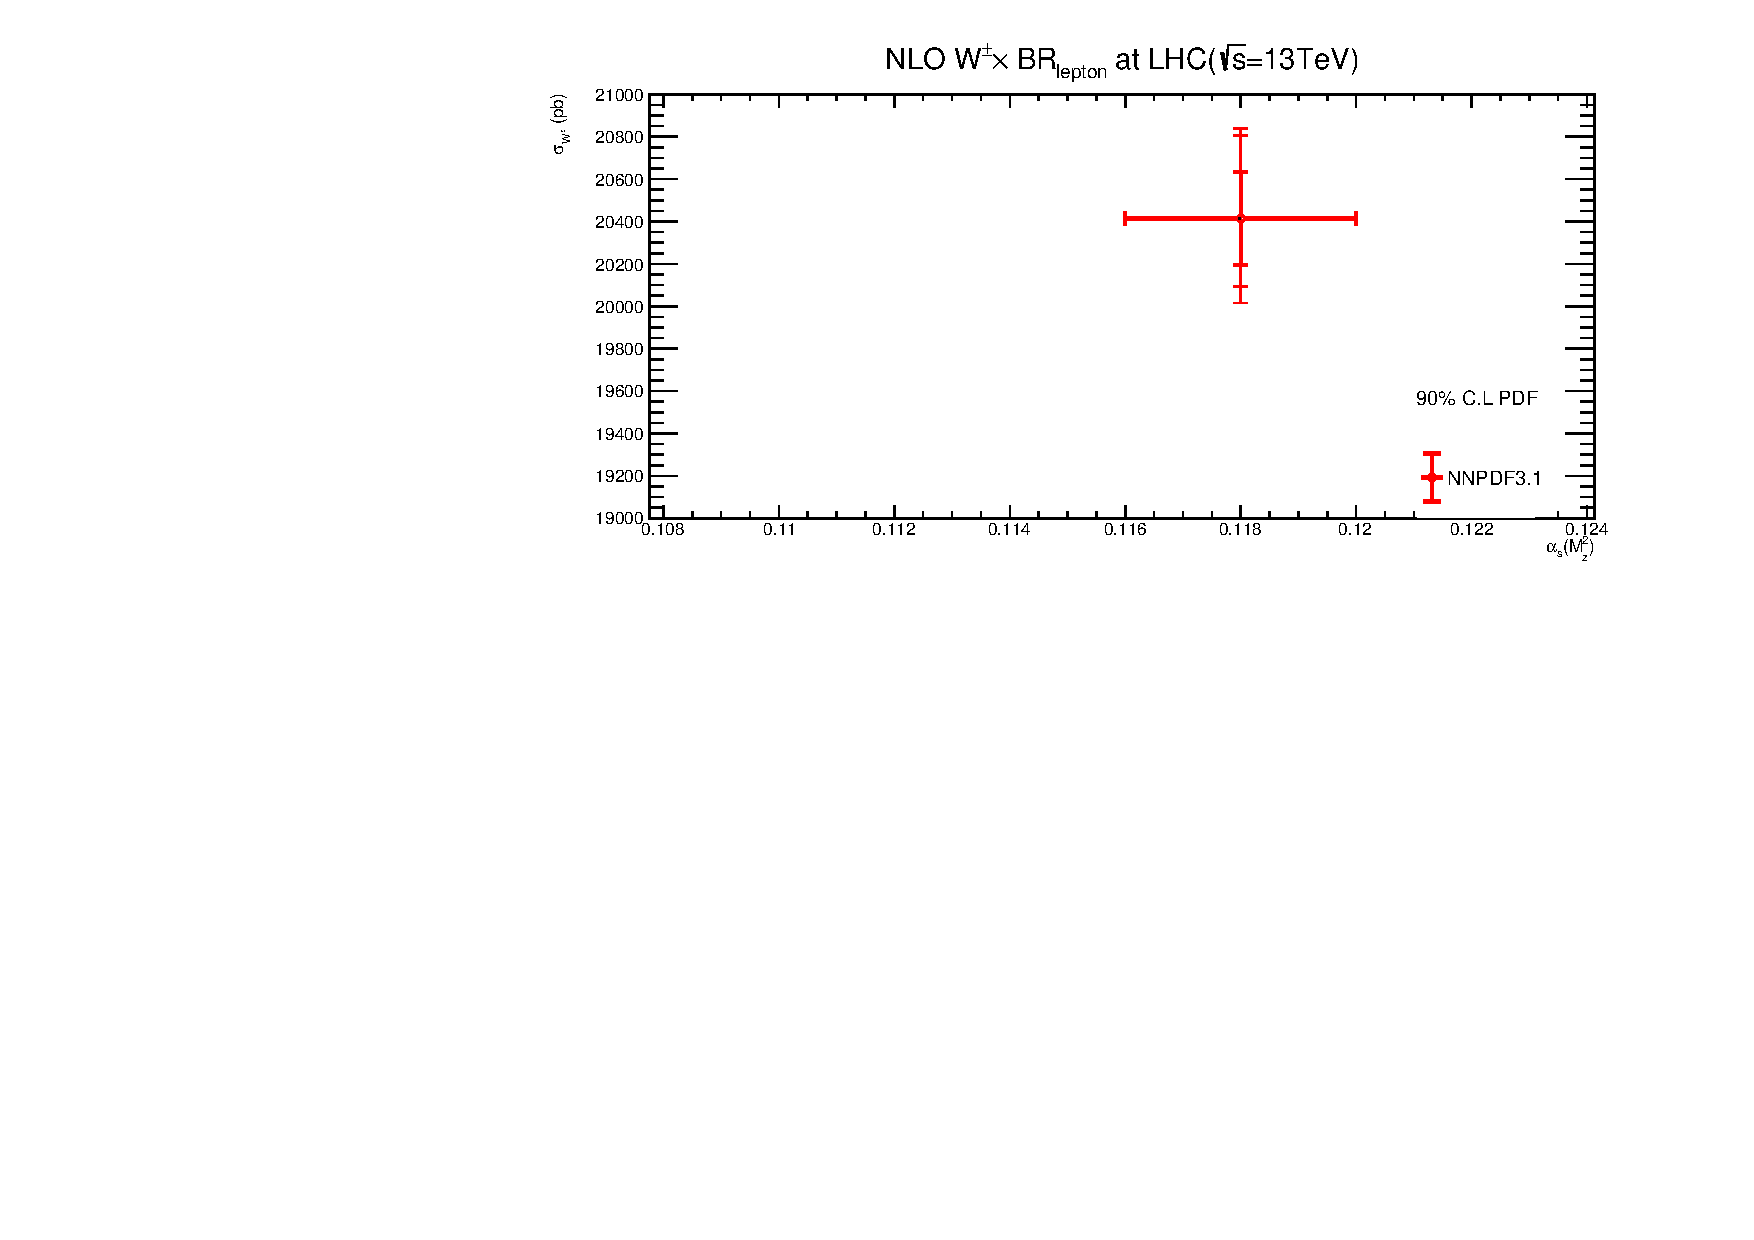
\includegraphics[height=5.6cm, width=\textwidth]{chapter4/Wnlo13.pdf}
\vspace*{-6mm}
\caption{}
\label{wnlo}

\end{subfigure}
\begin{subfigure}{0.49\textwidth}
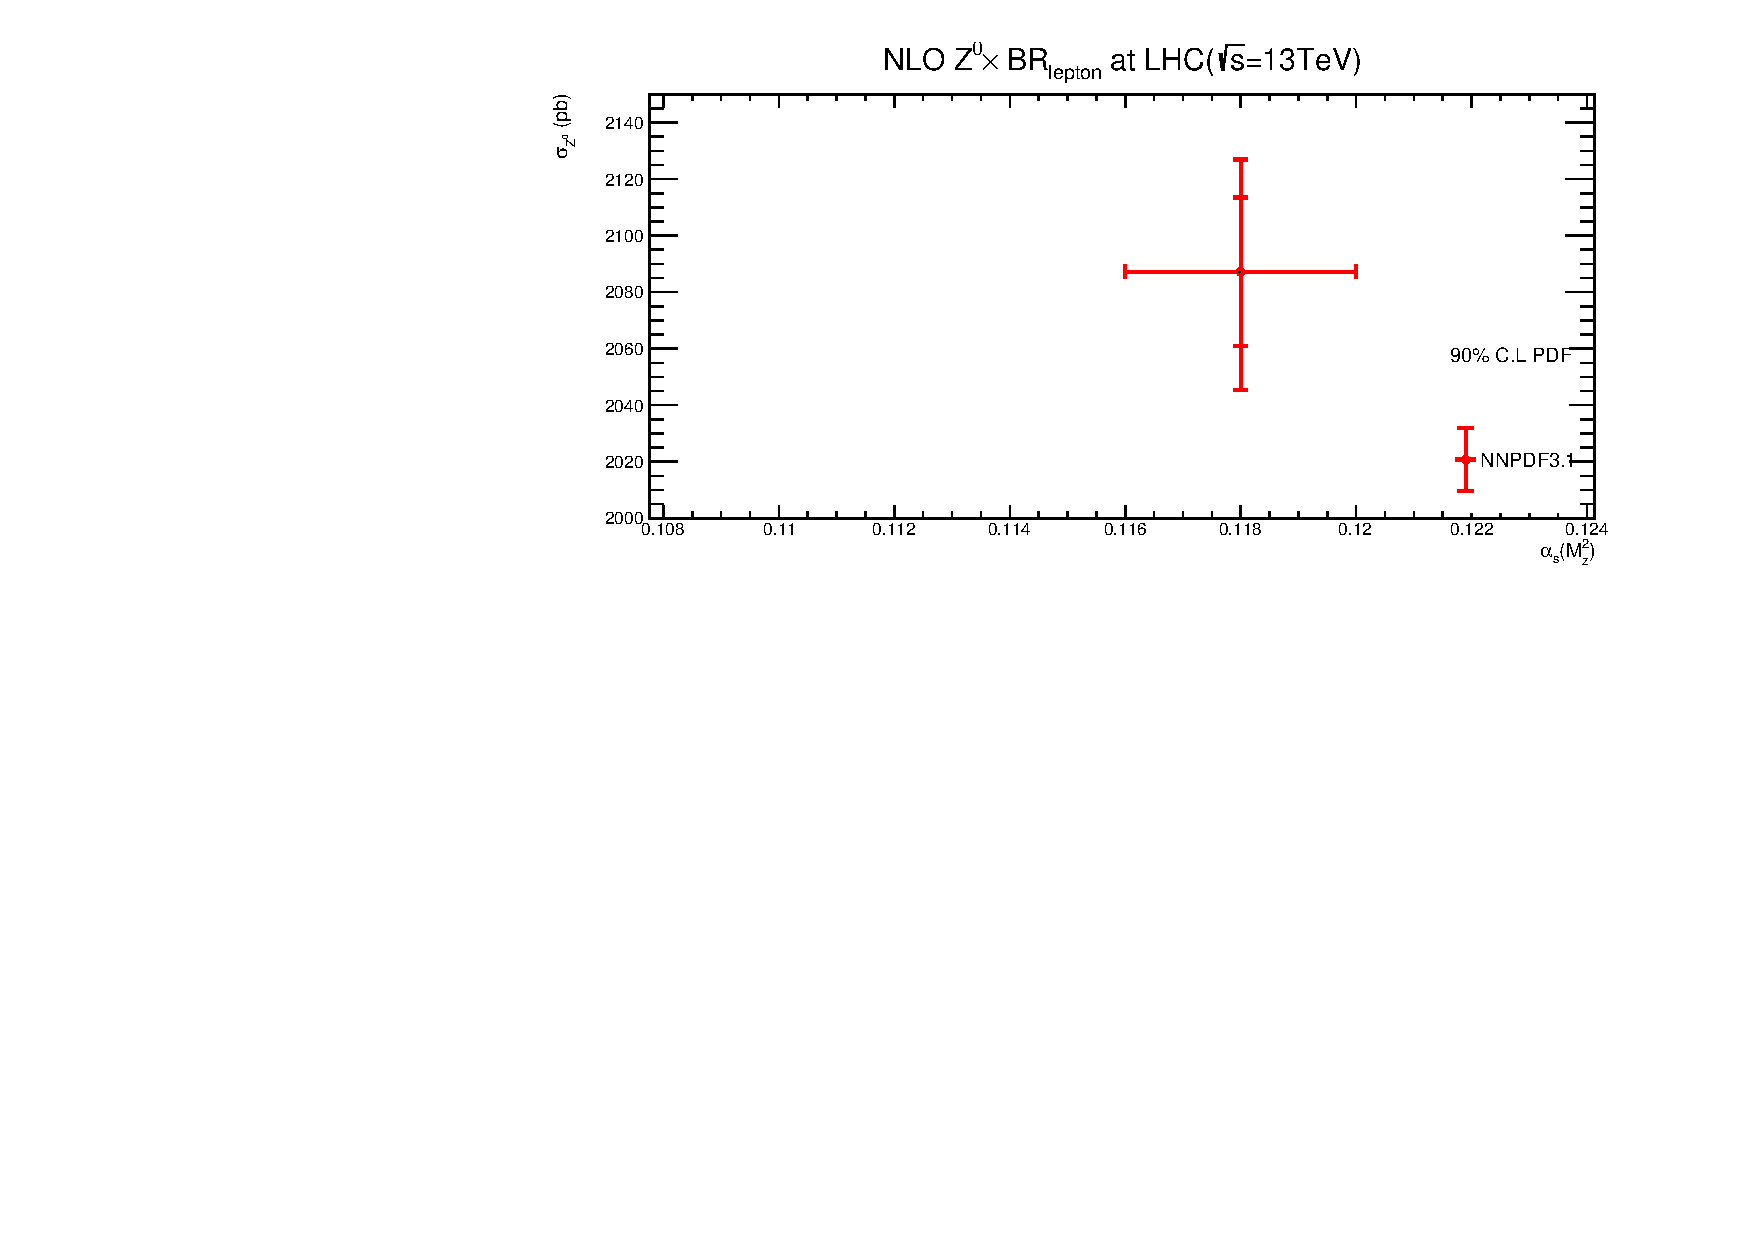
\includegraphics[height=5.6cm, width=\textwidth]{chapter4/Znlo13.pdf}
\vspace*{-6mm}
\caption{}
\label{znlo}
\end{subfigure}
\begin{subfigure}{0.49\textwidth}
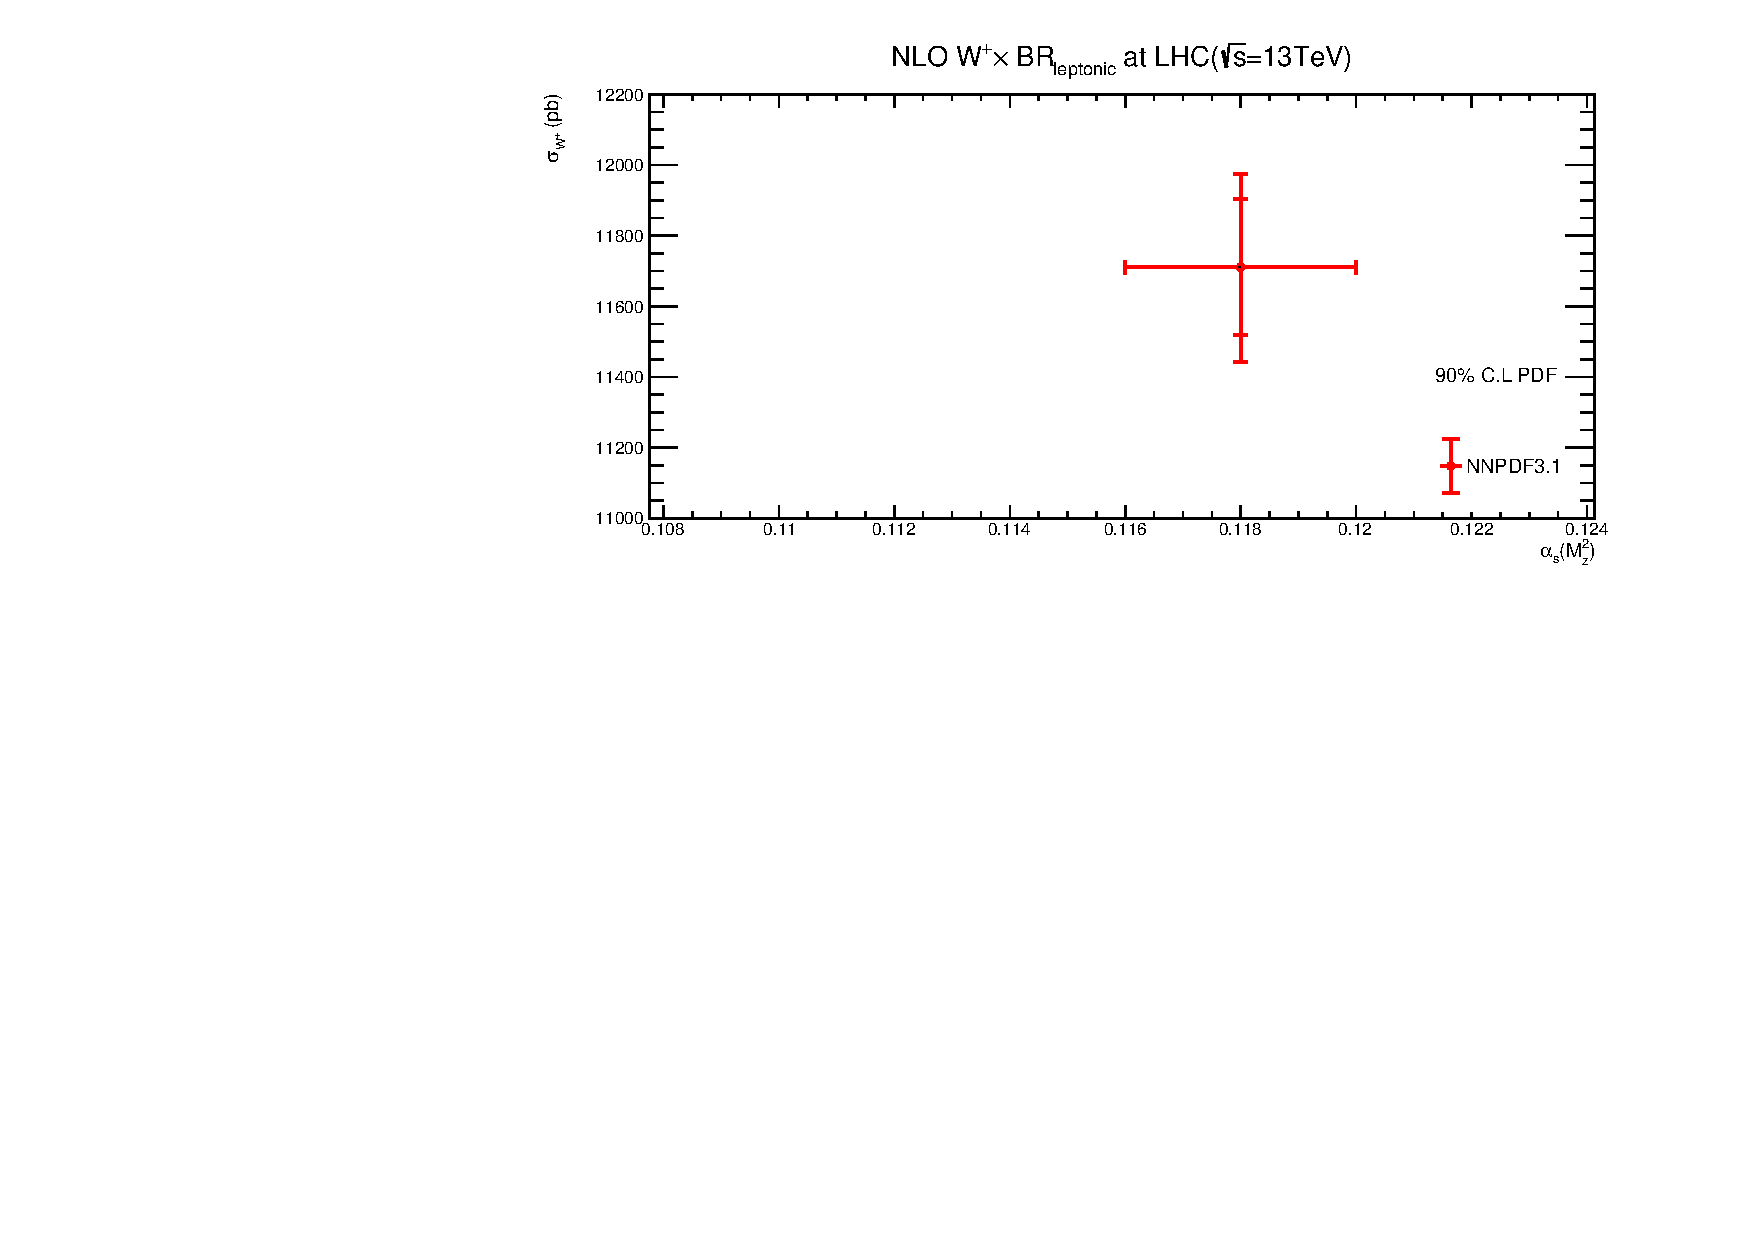
\includegraphics[height=5.6cm, width=\textwidth]{chapter4/Wpnlo13.pdf}
\vspace*{-6mm}
\caption{}
\label{wpnlo}
\end{subfigure}
\begin{subfigure}{0.49\textwidth}
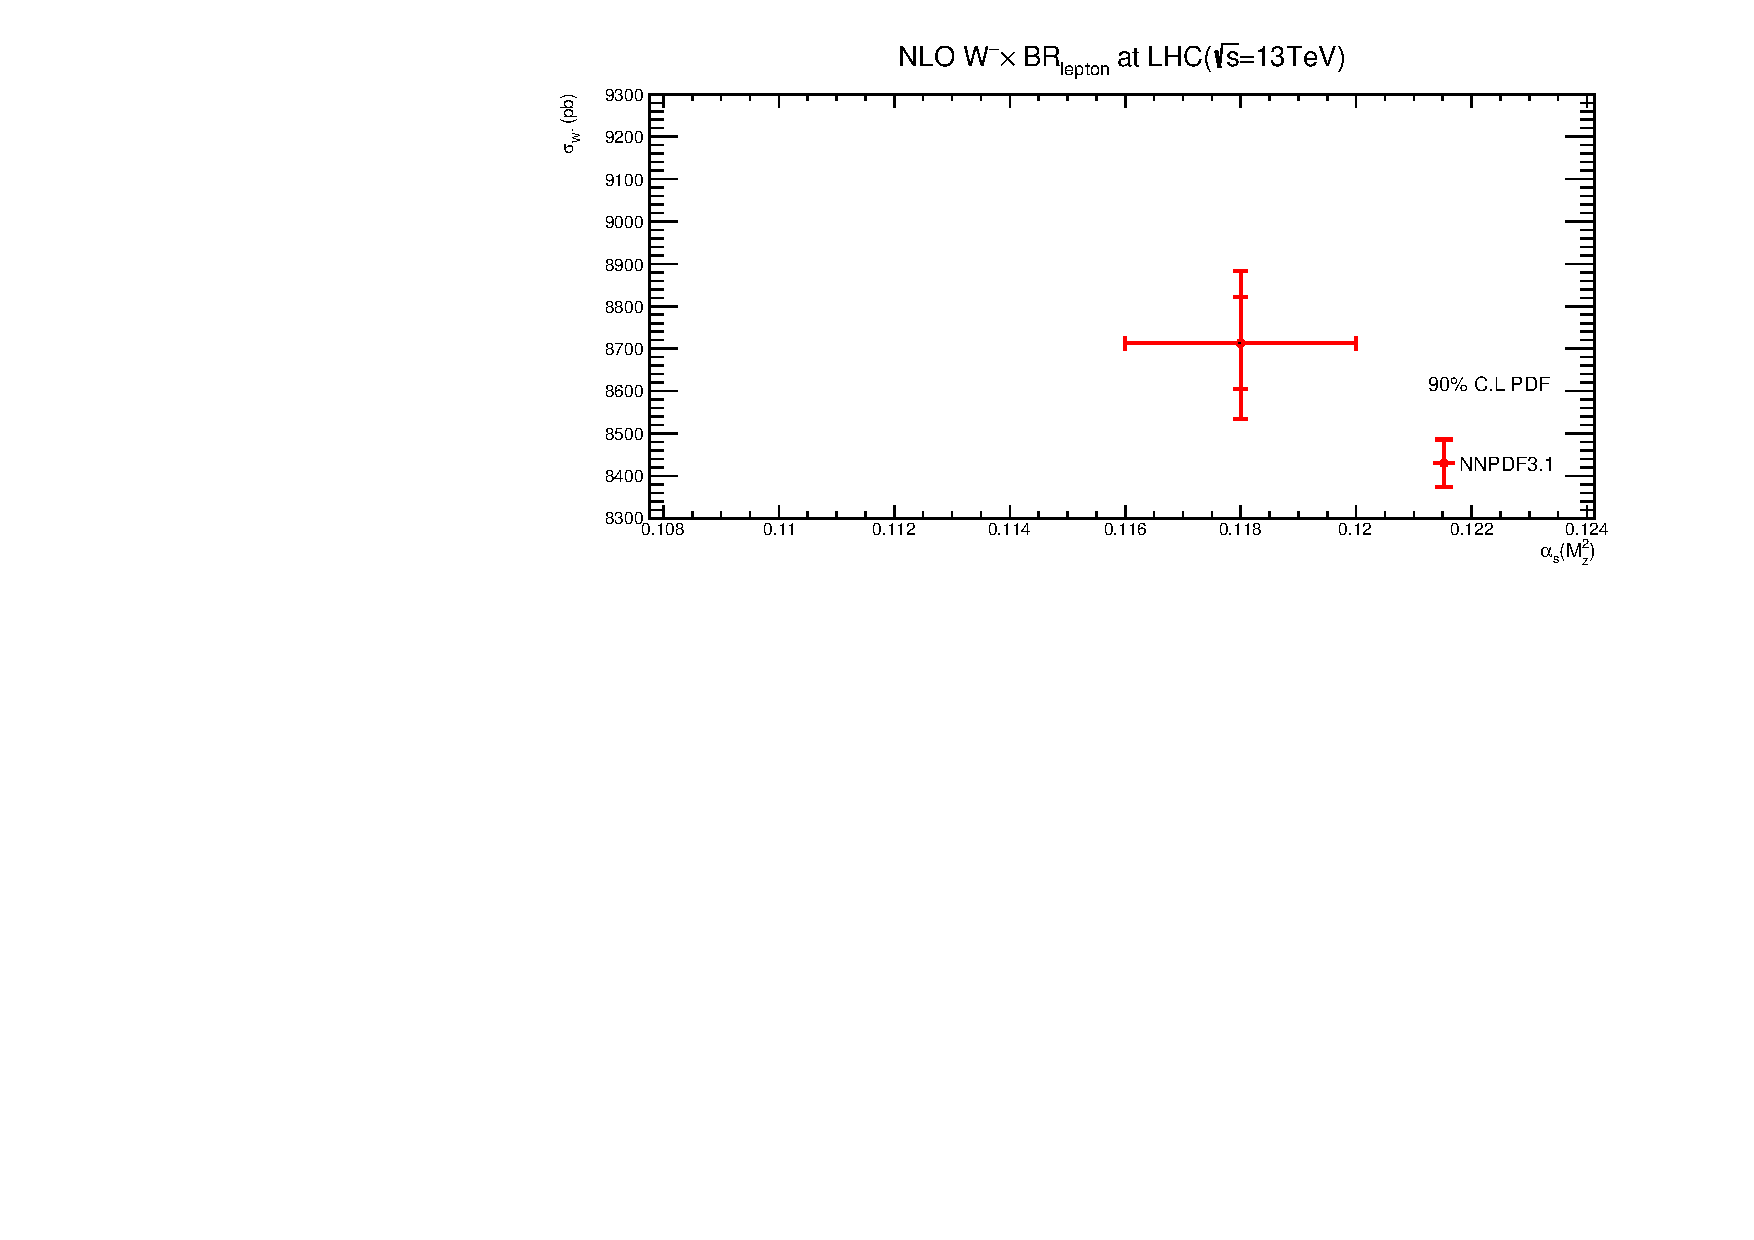
\includegraphics[height=5.6cm, width=\textwidth]{chapter4/Wmnlo13.pdf}
\vspace*{-6mm}
\caption{}
\label{wmnlo}
\end{subfigure}
\caption{\ref{wnlo} and \ref{znlo} are the NLO predictions of $W$ and $Z$ boson at $13TeV$, \ref{wpnlo} and \ref{wmnlo} are for the $W^{+}$ and $W^{-}$ bosons at $13~TeV$.}
\label{NLO_WZ}
\end{figure}


\begin{figure}[H]{\label{WZ13_14}}
\centering
\begin{subfigure}{0.49\textwidth}
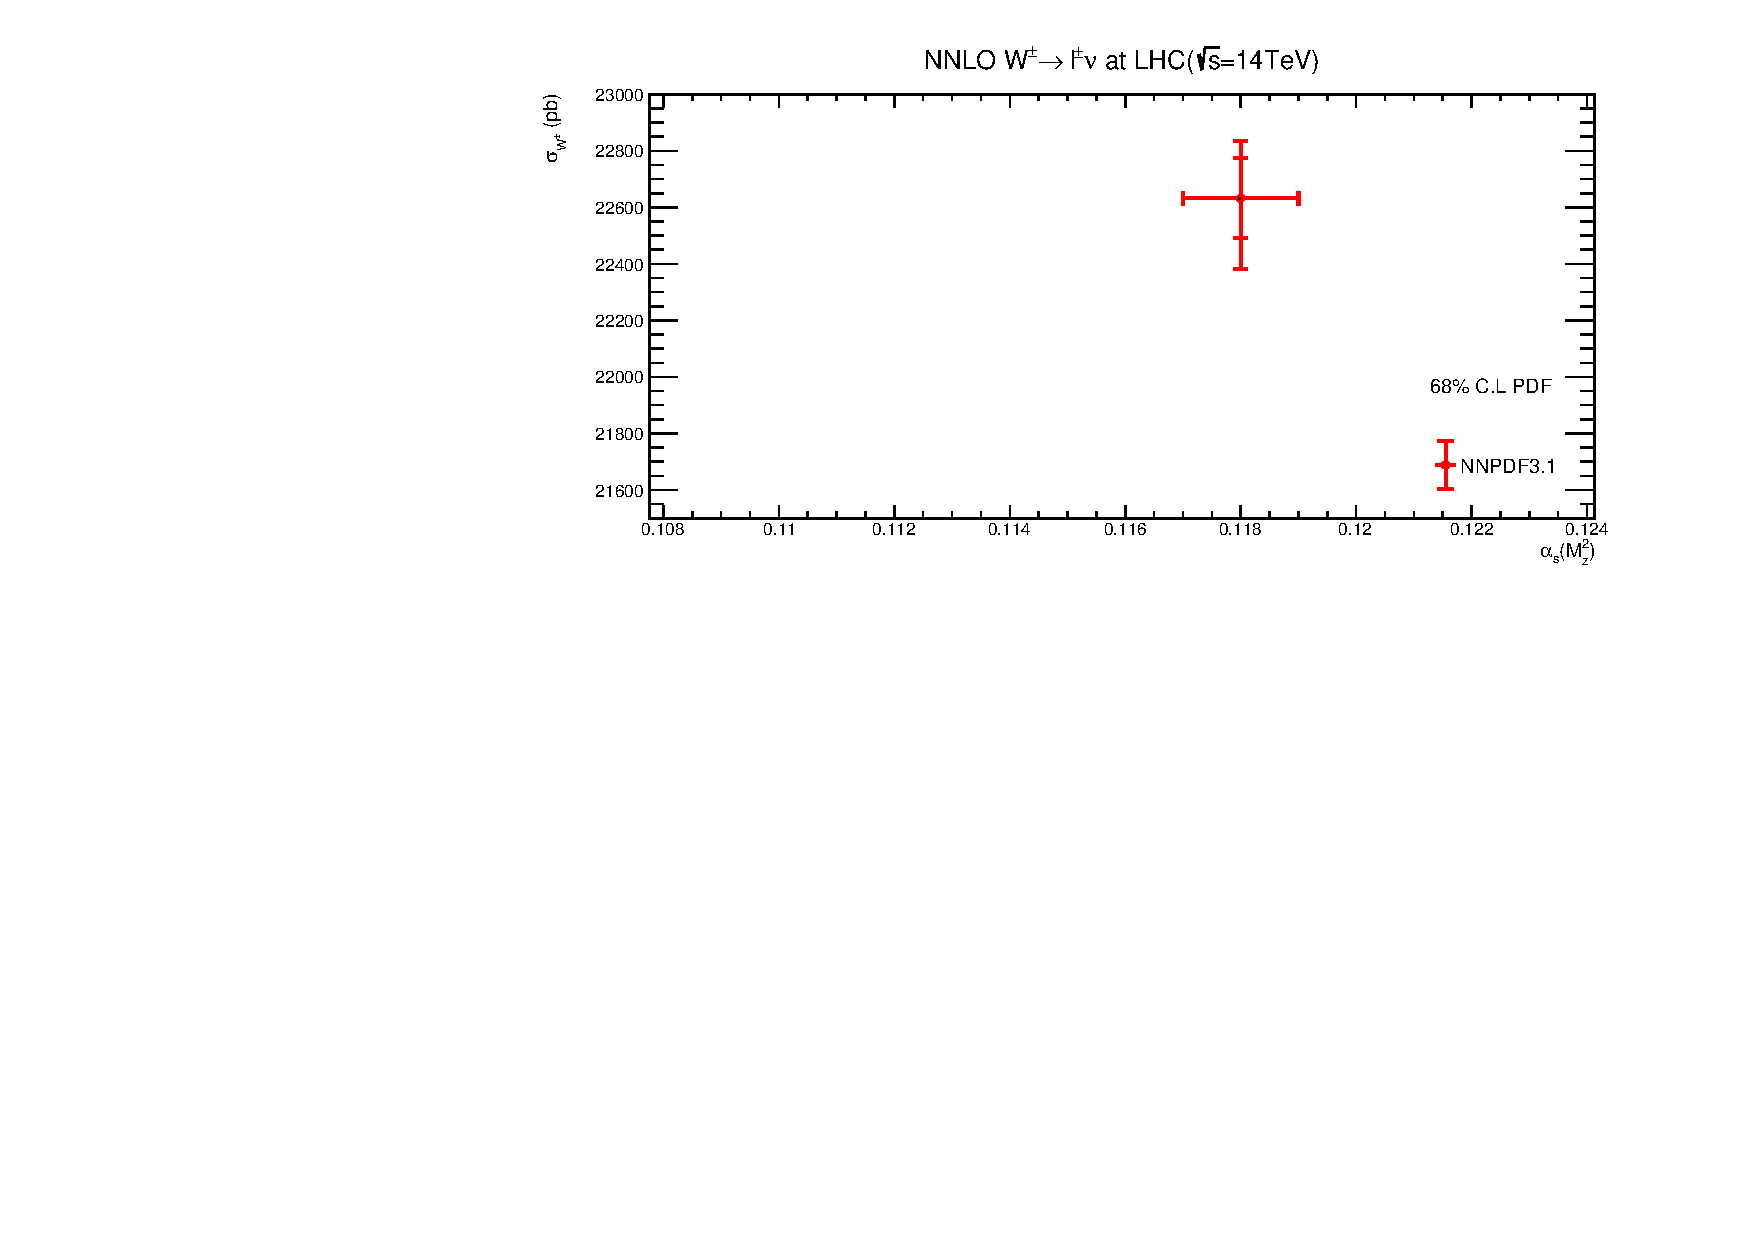
\includegraphics[height=6cm ,width=\textwidth]{chapter4/W14.pdf}
\vspace*{-6mm}
\caption{}
\label{w14}
\end{subfigure}
\begin{subfigure}{0.49\textwidth}
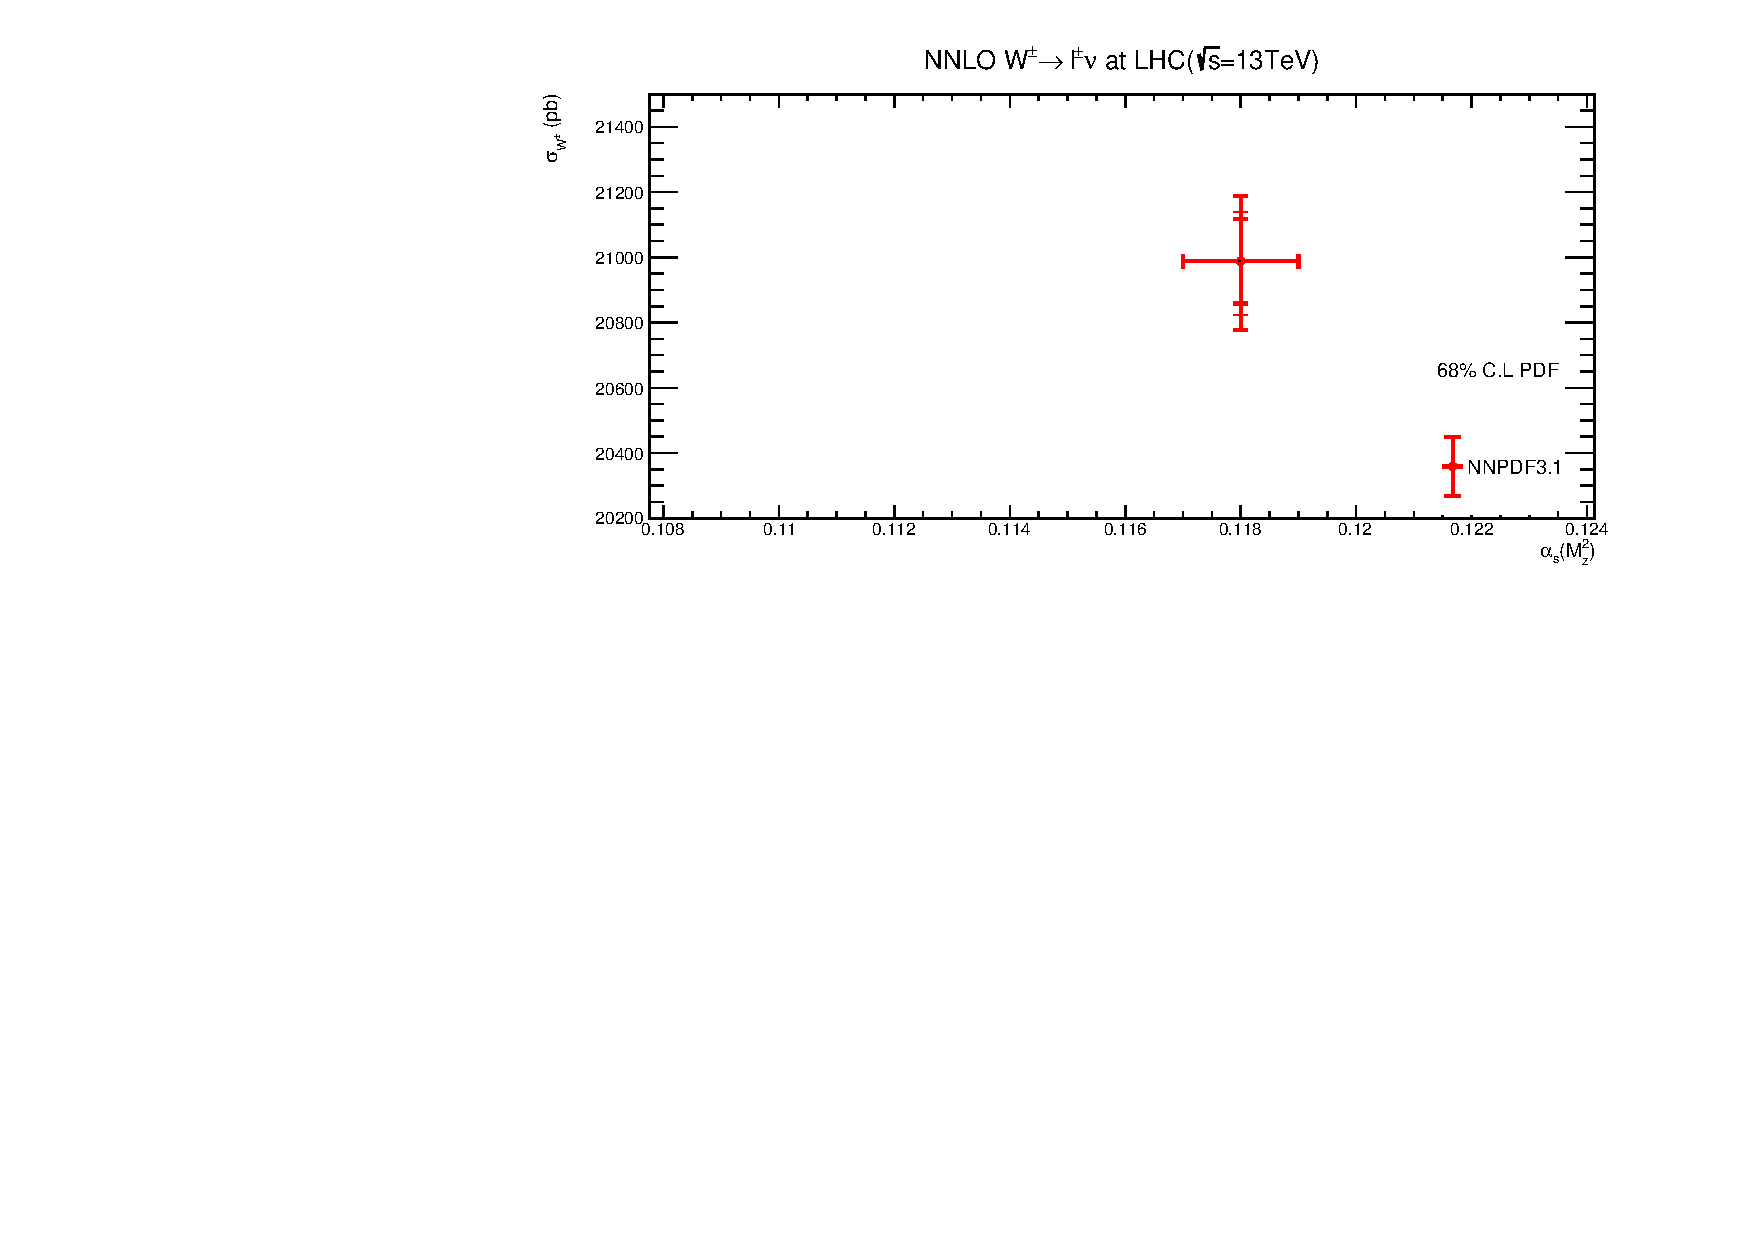
\includegraphics[height=6cm, width=\textwidth]{chapter4/W13.pdf}
\vspace*{-6mm}
\caption{}
\label{w13}
\end{subfigure}
\begin{subfigure}{0.49\textwidth}
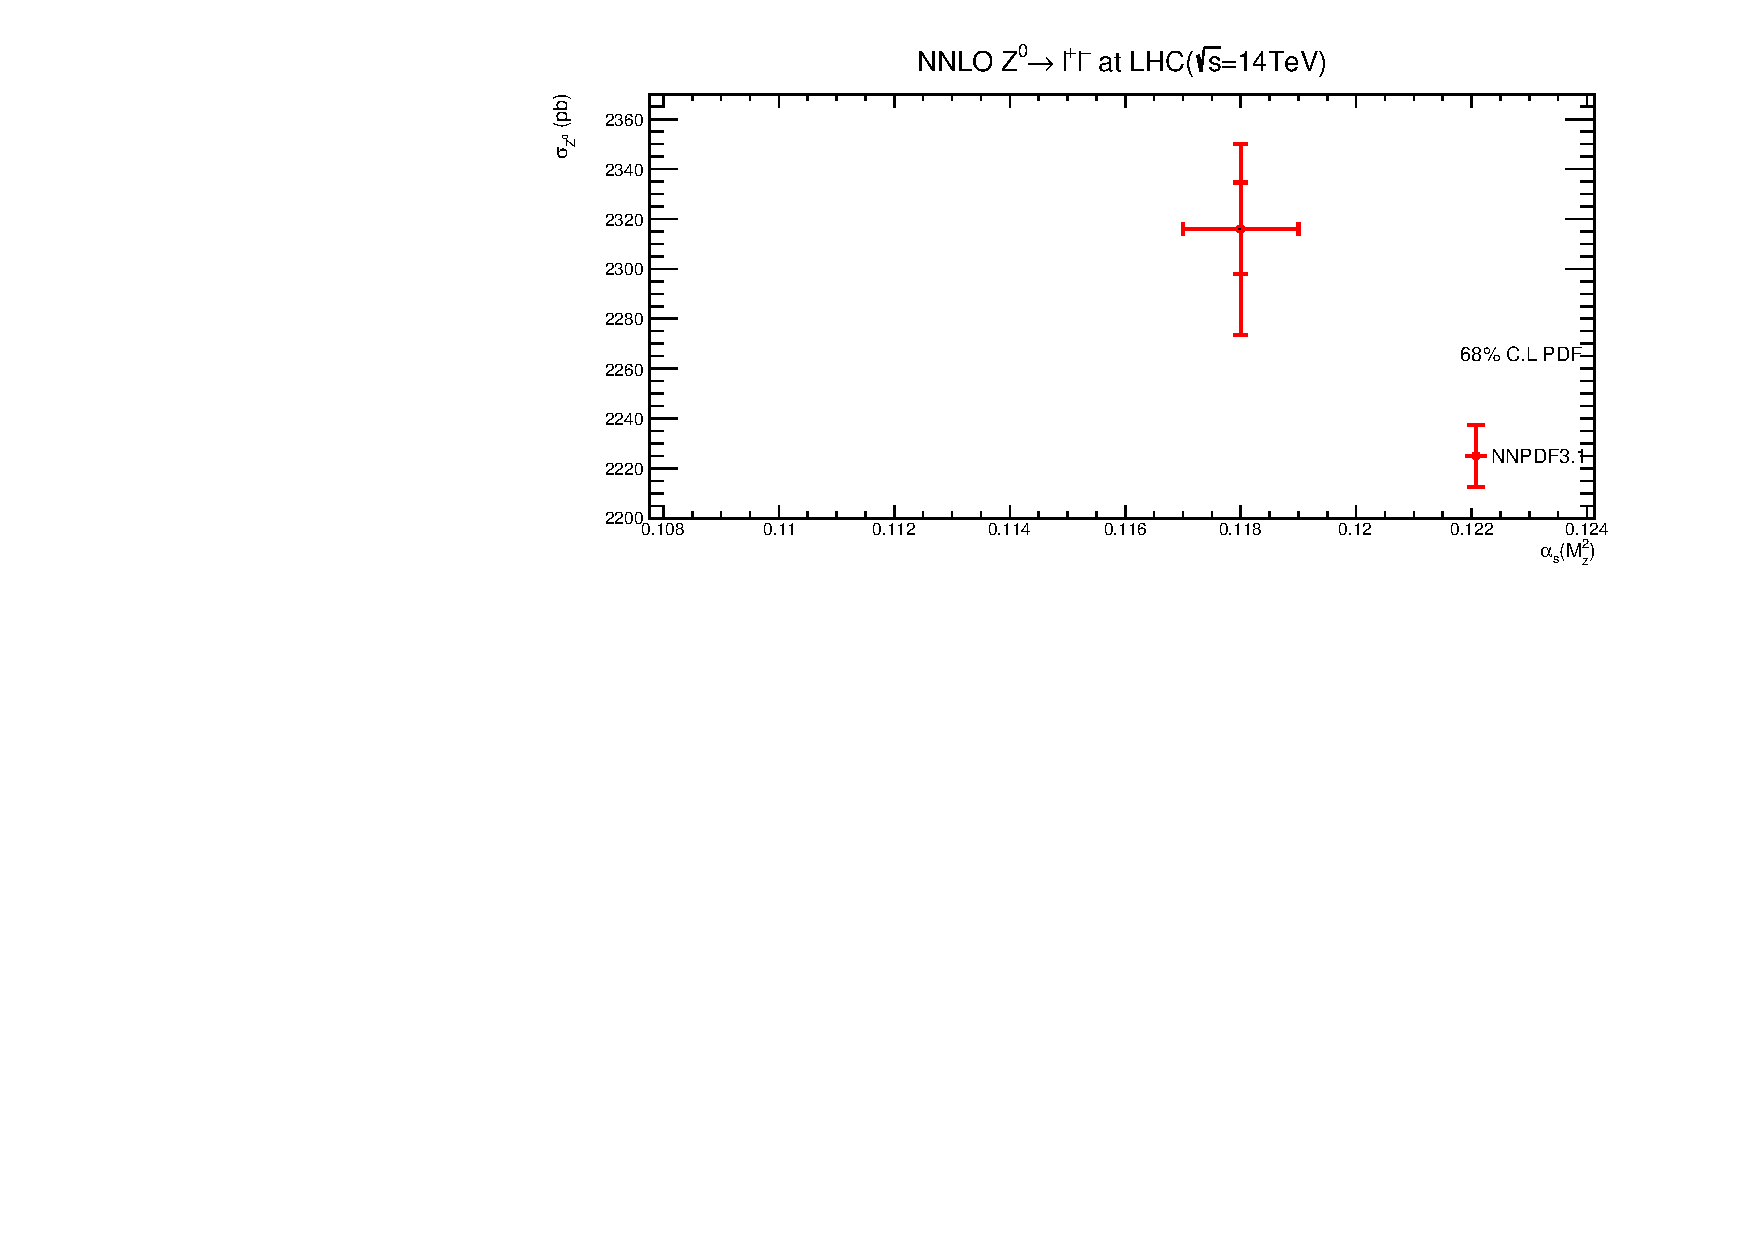
\includegraphics[height=6cm, width=\textwidth]{chapter4/Z14.pdf}
\vspace*{-6mm}
\caption{}
\label{z14}
\end{subfigure}
\begin{subfigure}{0.49\textwidth}
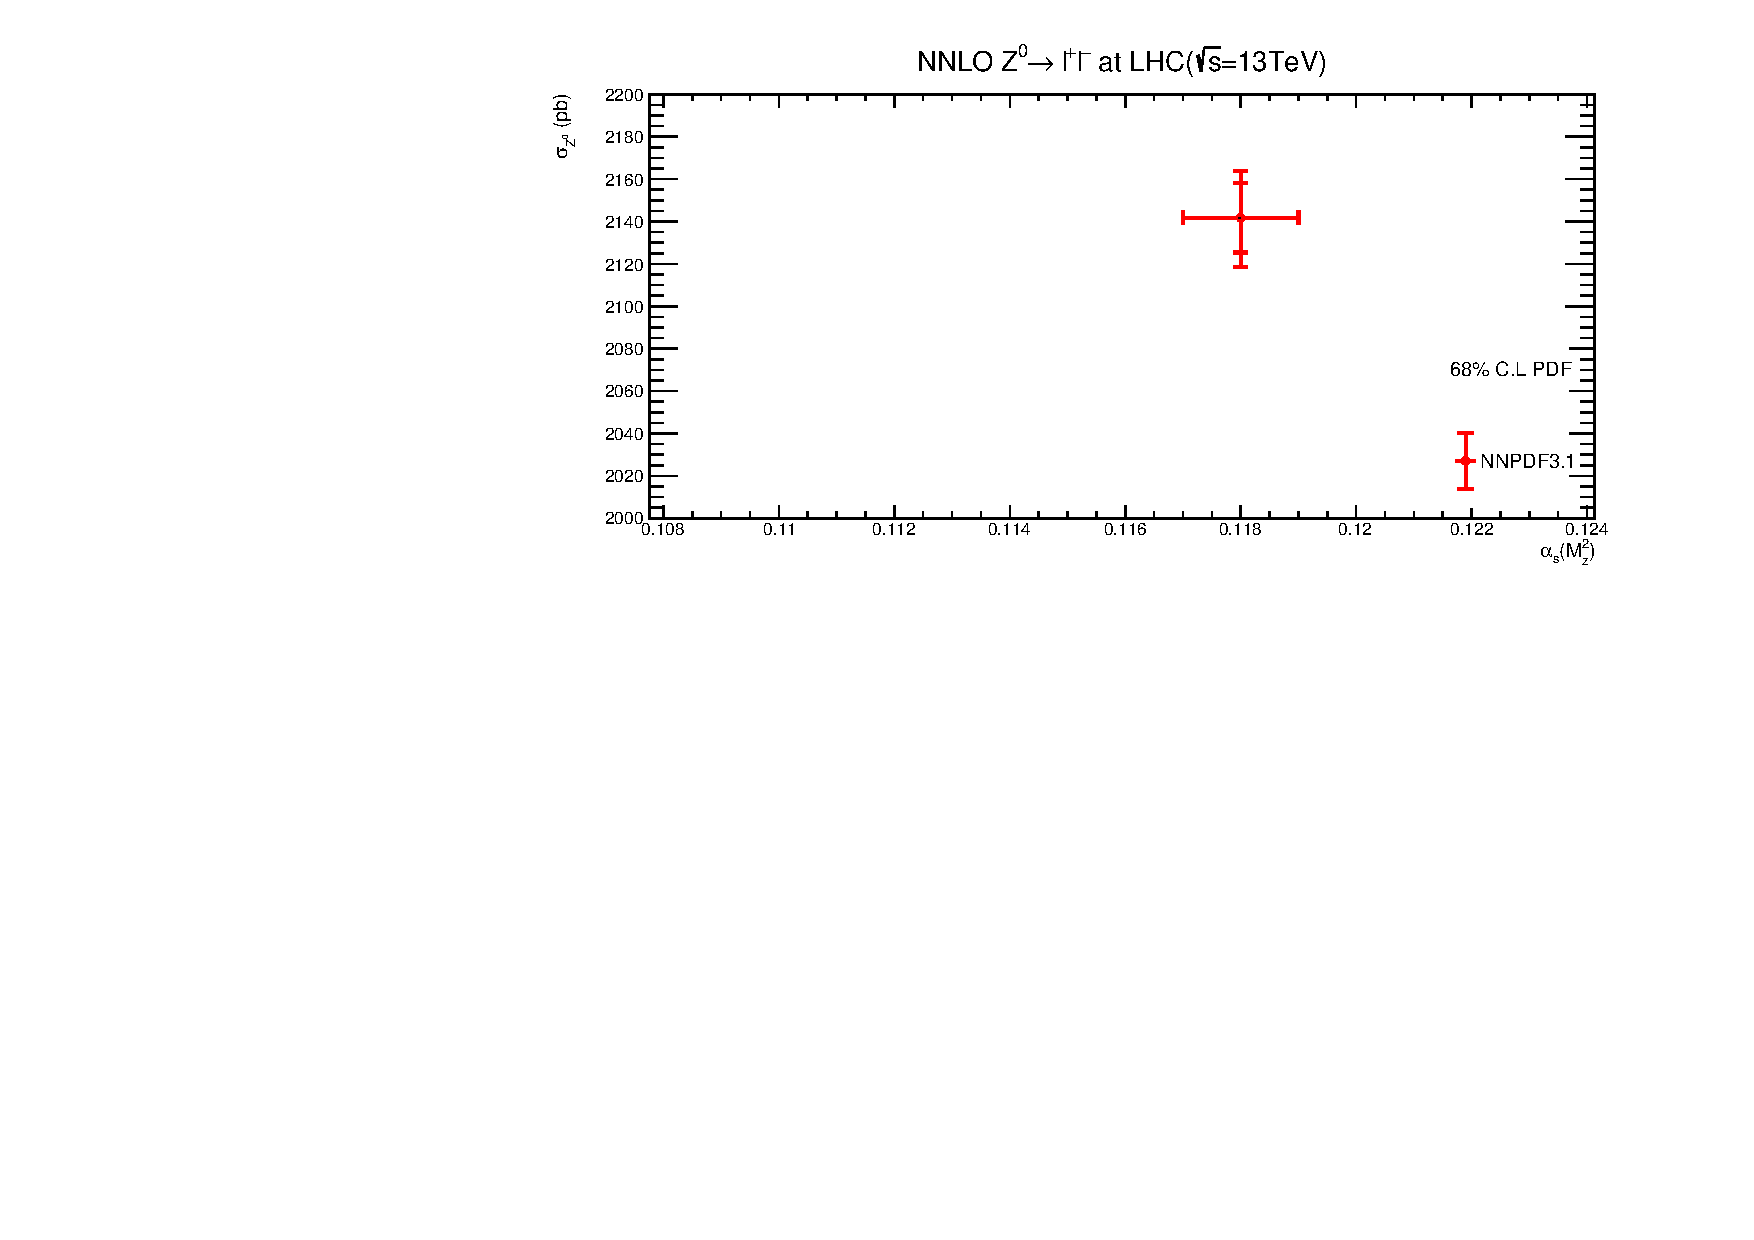
\includegraphics[height=6cm, width=\textwidth]{chapter4/Z13.pdf}
\vspace*{-6mm}
\caption{}
\label{z13}
\end{subfigure}
\begin{subfigure}{0.49\textwidth}
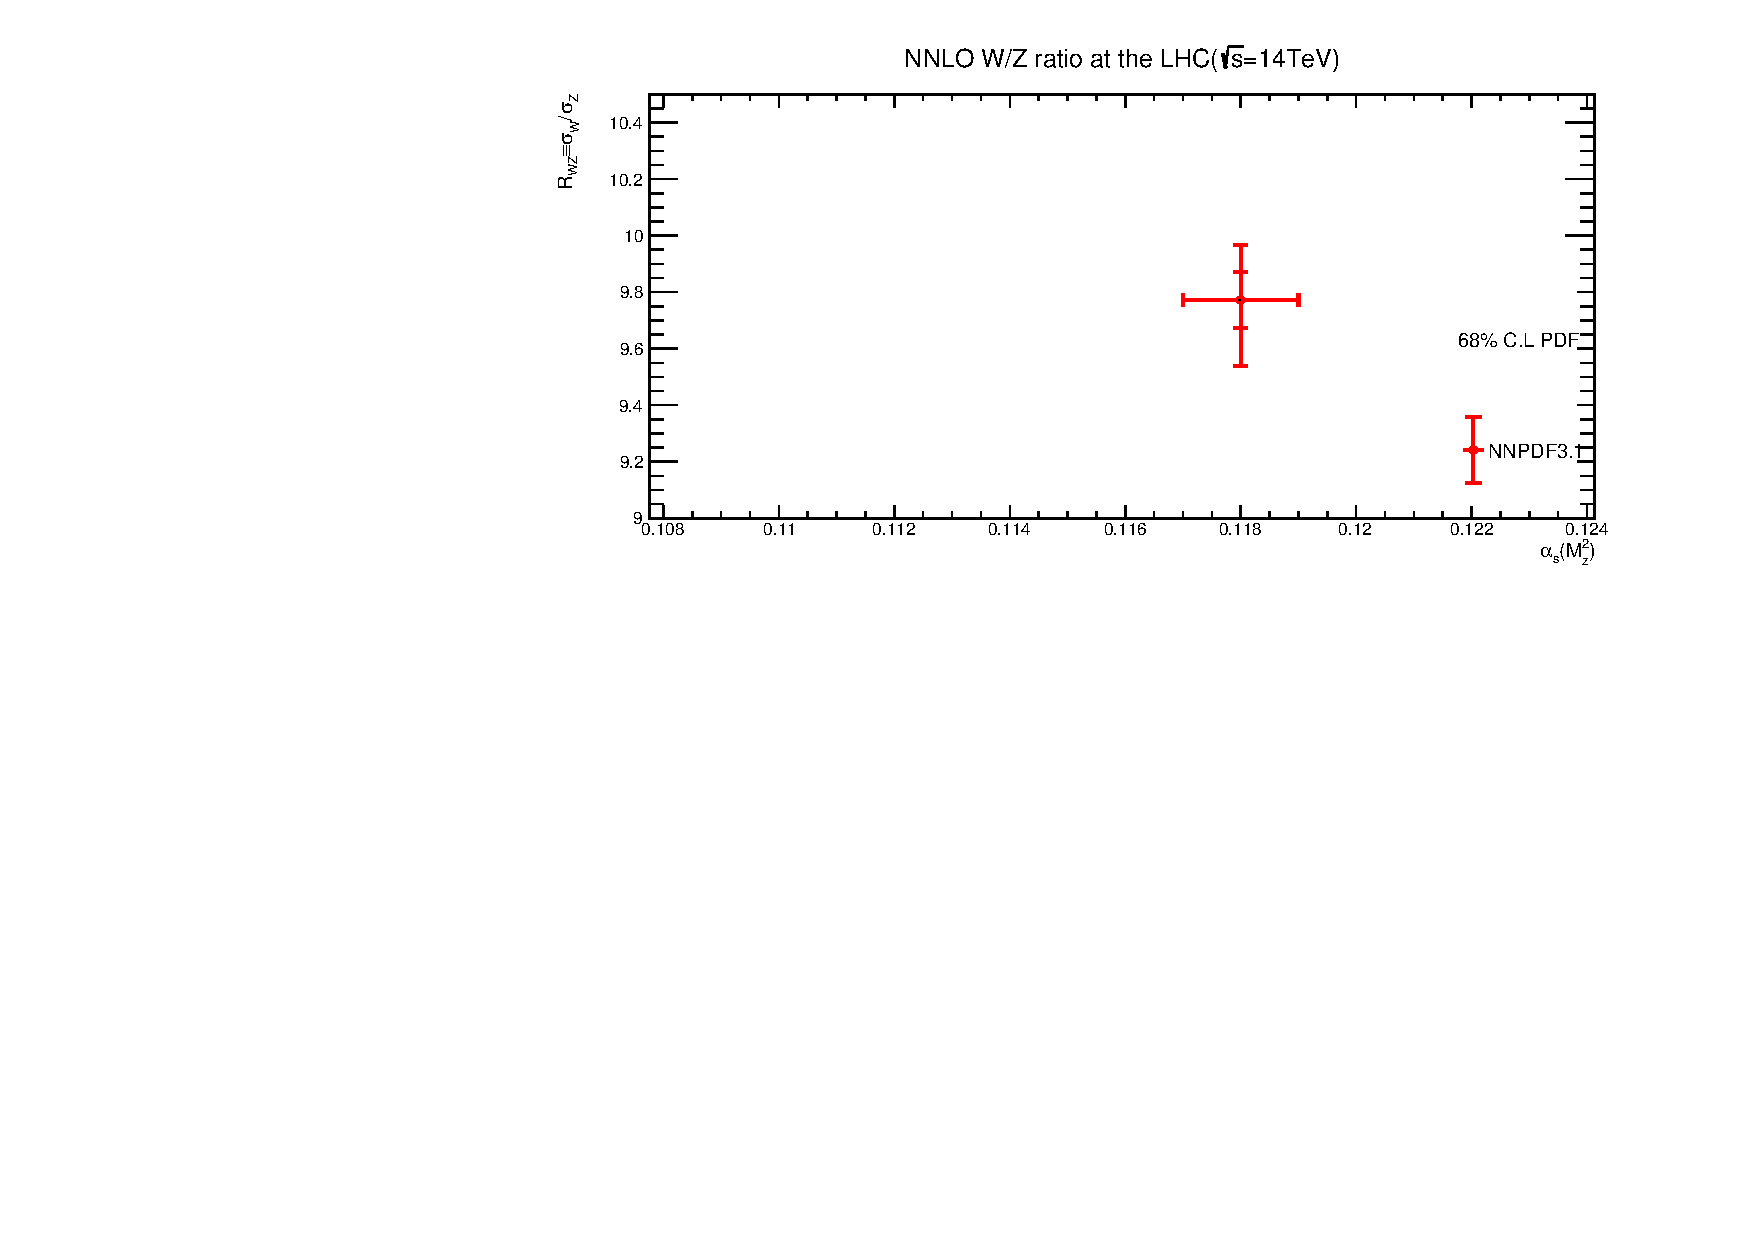
\includegraphics[height=6cm, width=\textwidth]{chapter4/Rwz14.pdf}
\vspace*{-6mm}
\caption{}
\label{rwz14}
\end{subfigure}
\begin{subfigure}{0.49\textwidth}
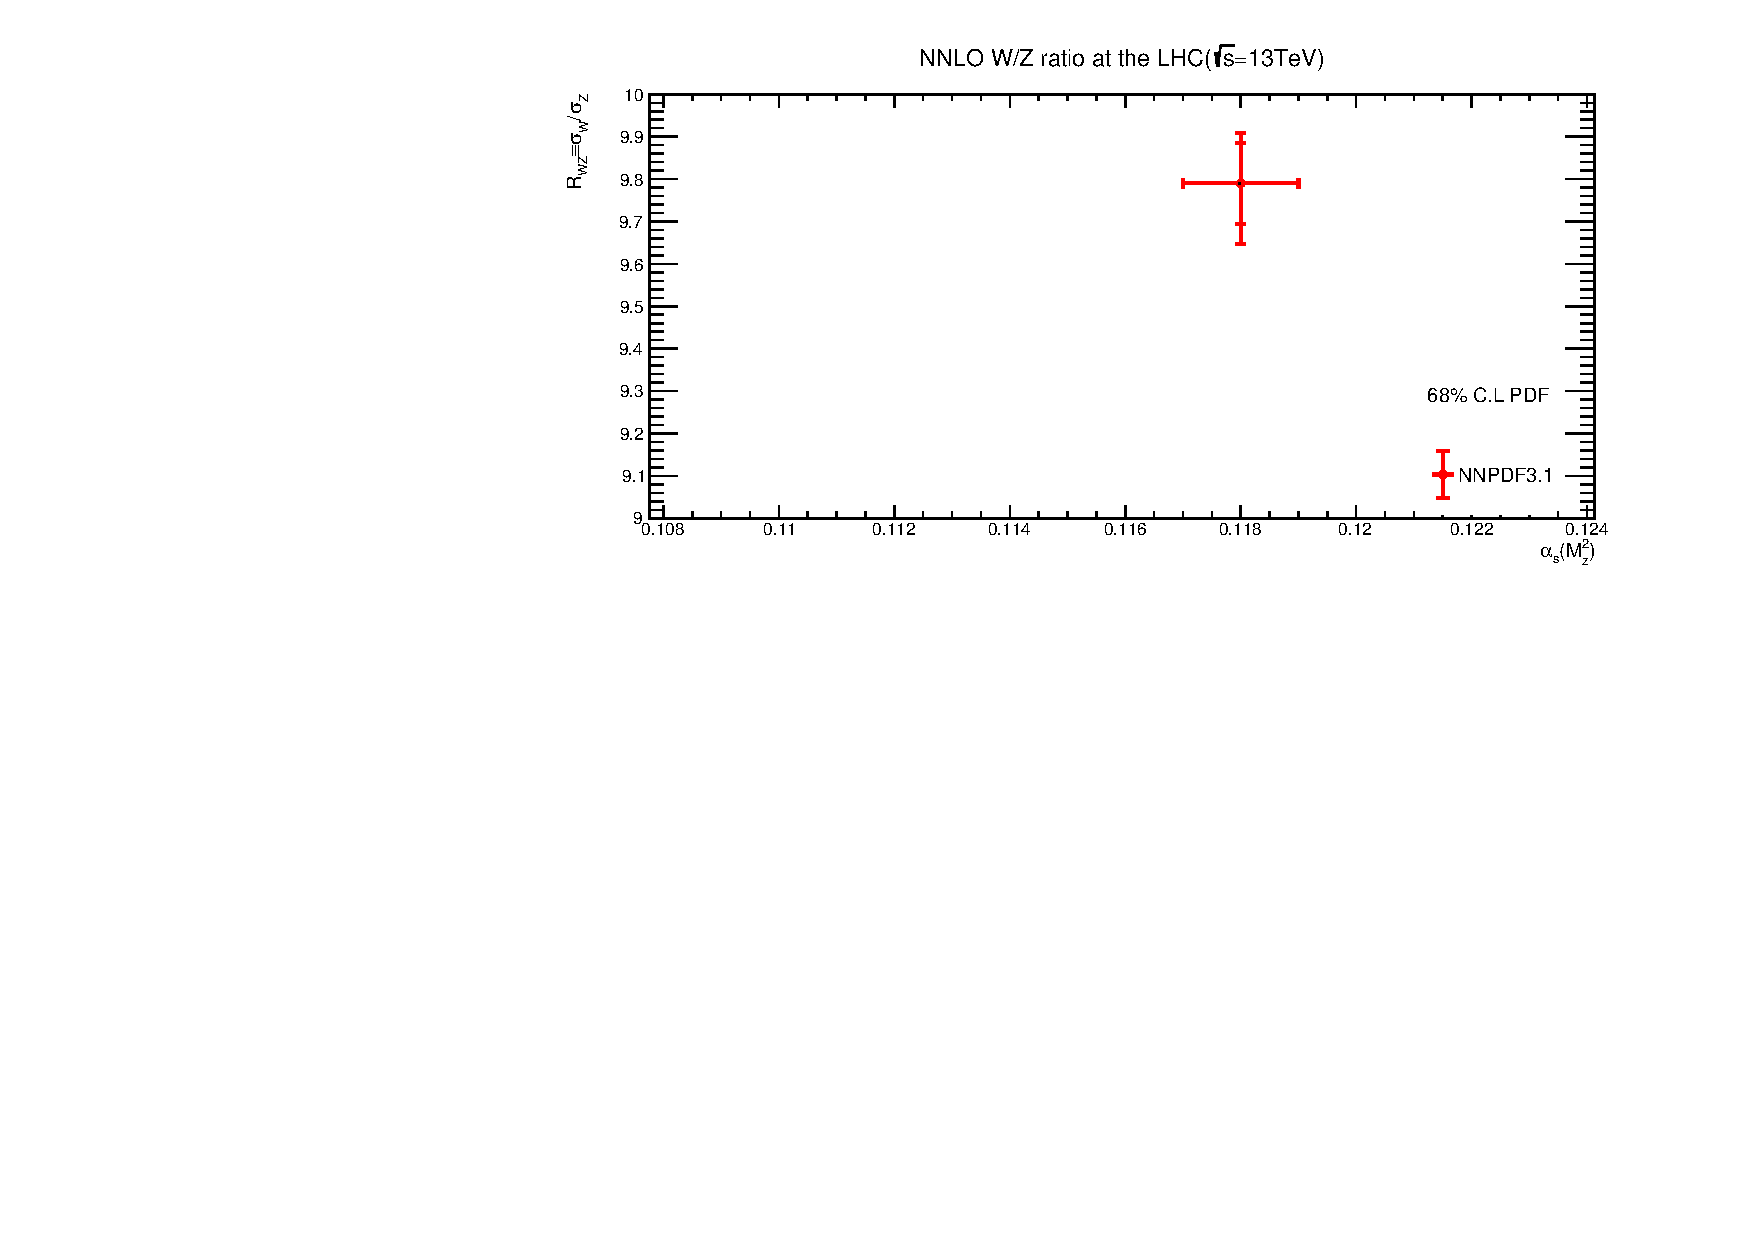
\includegraphics[height=6cm, width=\textwidth]{chapter4/Rwz13.pdf}
\vspace*{-6mm}
\caption{}
\label{rwz13}
\end{subfigure}
\caption{In Figure:~\ref{w14}~\ref{w13} are the NNLO predictions of $W$ boson production cross section at $13~TeV$ and $14~TeV$ with $68\%$ C.L. uncertainties. \ref{z14}~\ref{z13} are the $Z$ boson production cross section and \ref{rwz14}~\ref{rwz13} are the predicted ratio of $W$ and $Z$ boson production cross section at $13TeV$ and $14TeV$. The vertical error bars on prediction represent: inner~(PDF),~middle~($\alpha_{s}$),~outer~(PDF+$\alpha_{s}$~combined) error.} 
\label{13tev1}
\end{figure}


\begin{figure}[H]
\centering
\begin{subfigure}{0.49\textwidth}
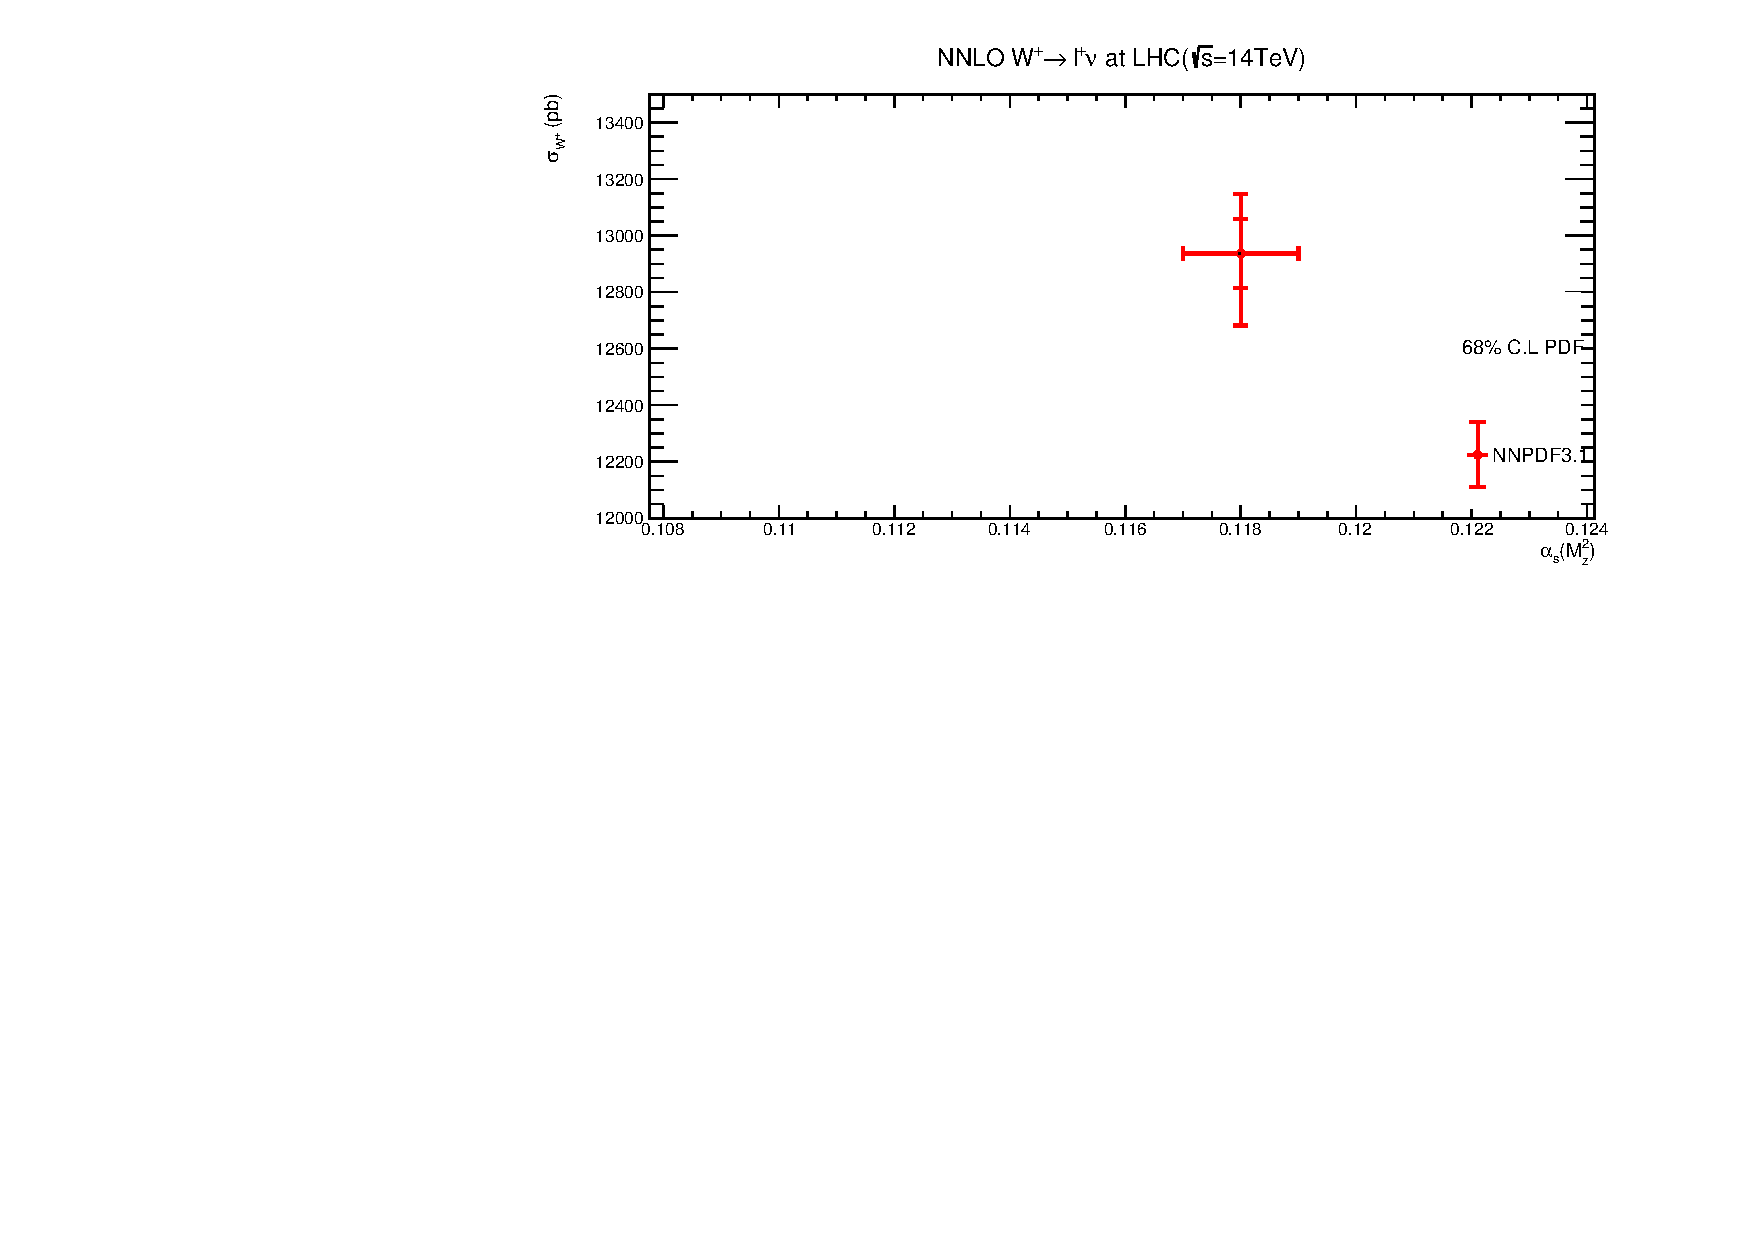
\includegraphics[height=6cm ,width=\textwidth]{chapter4/Wp14.pdf}

\caption{}
\label{w+14}
\end{subfigure}
\begin{subfigure}{0.49\textwidth}
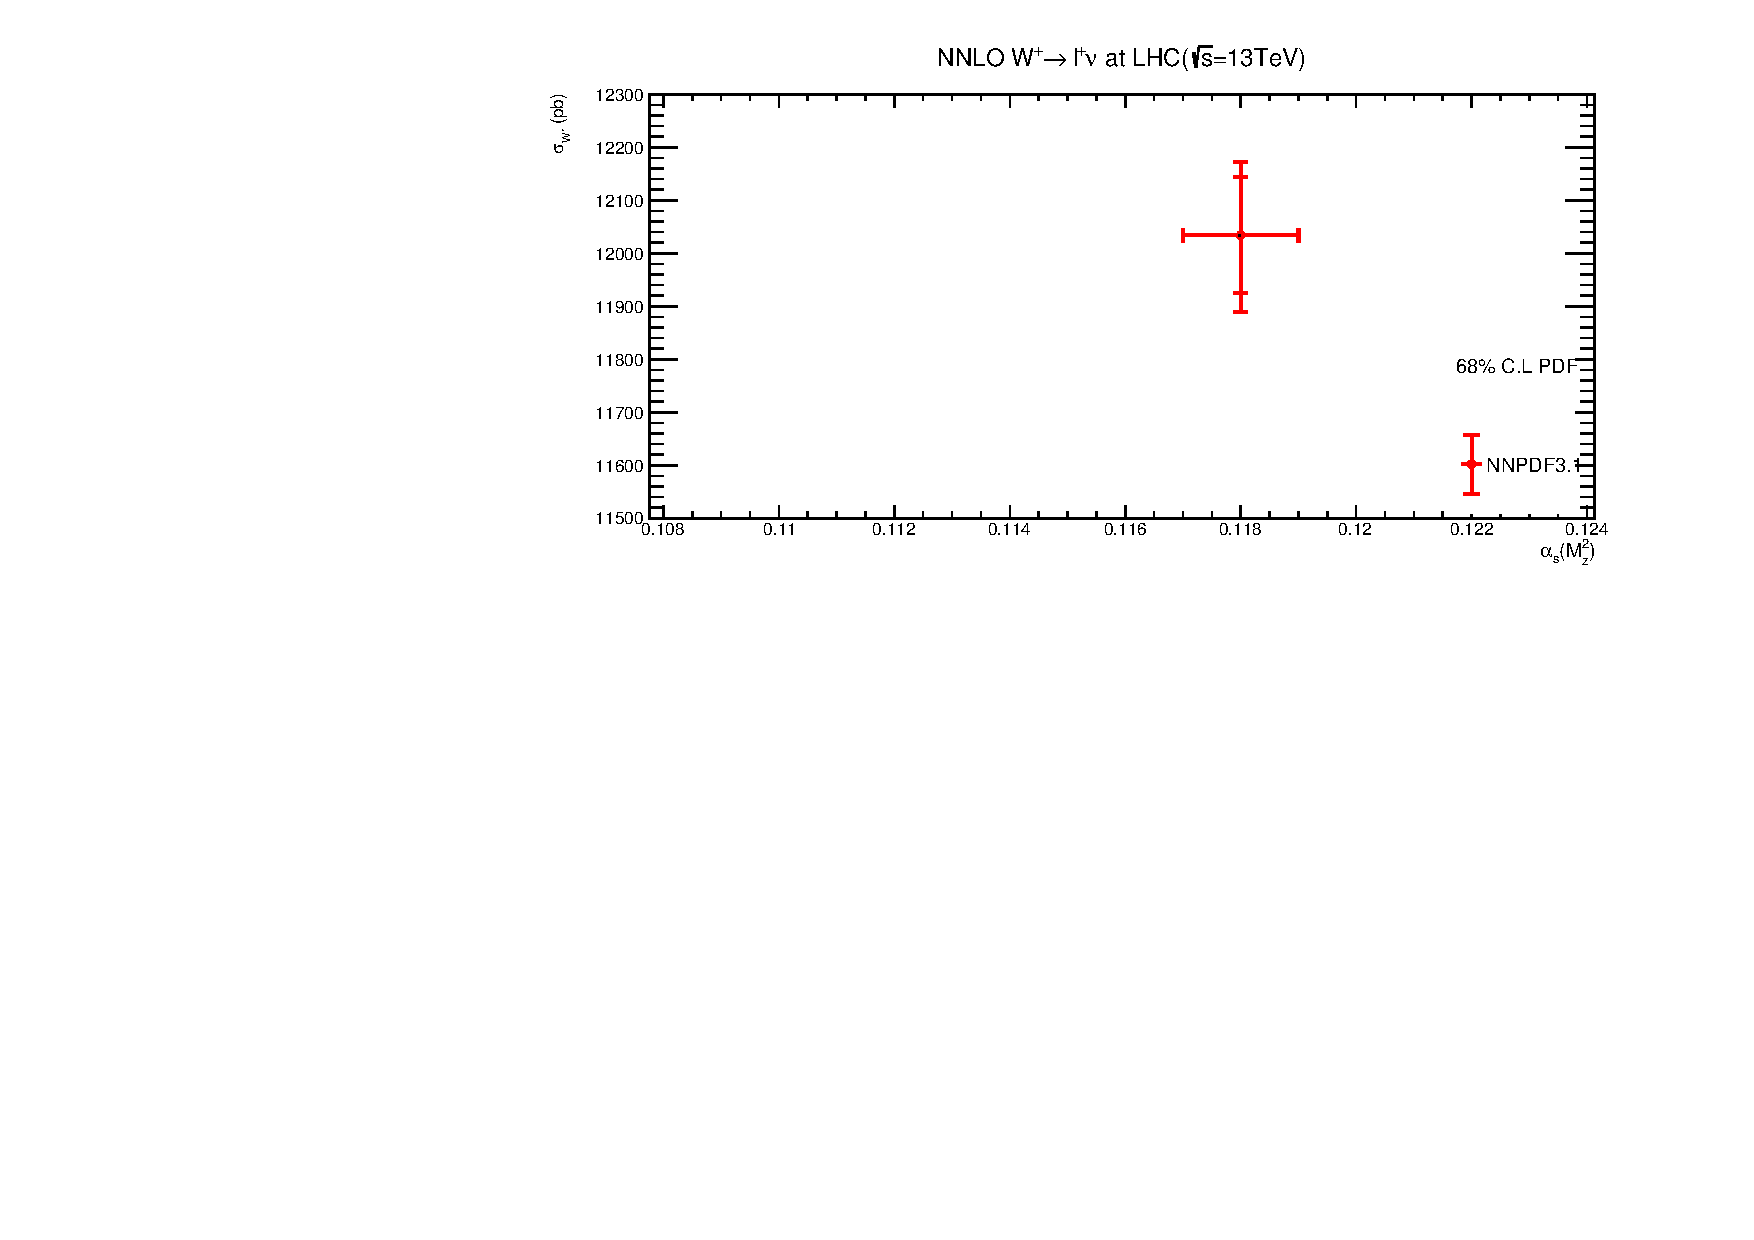
\includegraphics[height=6cm, width=\textwidth]{chapter4/Wp13.pdf}
\caption{}
\label{w+13}
\end{subfigure}
\begin{subfigure}{0.49\textwidth}
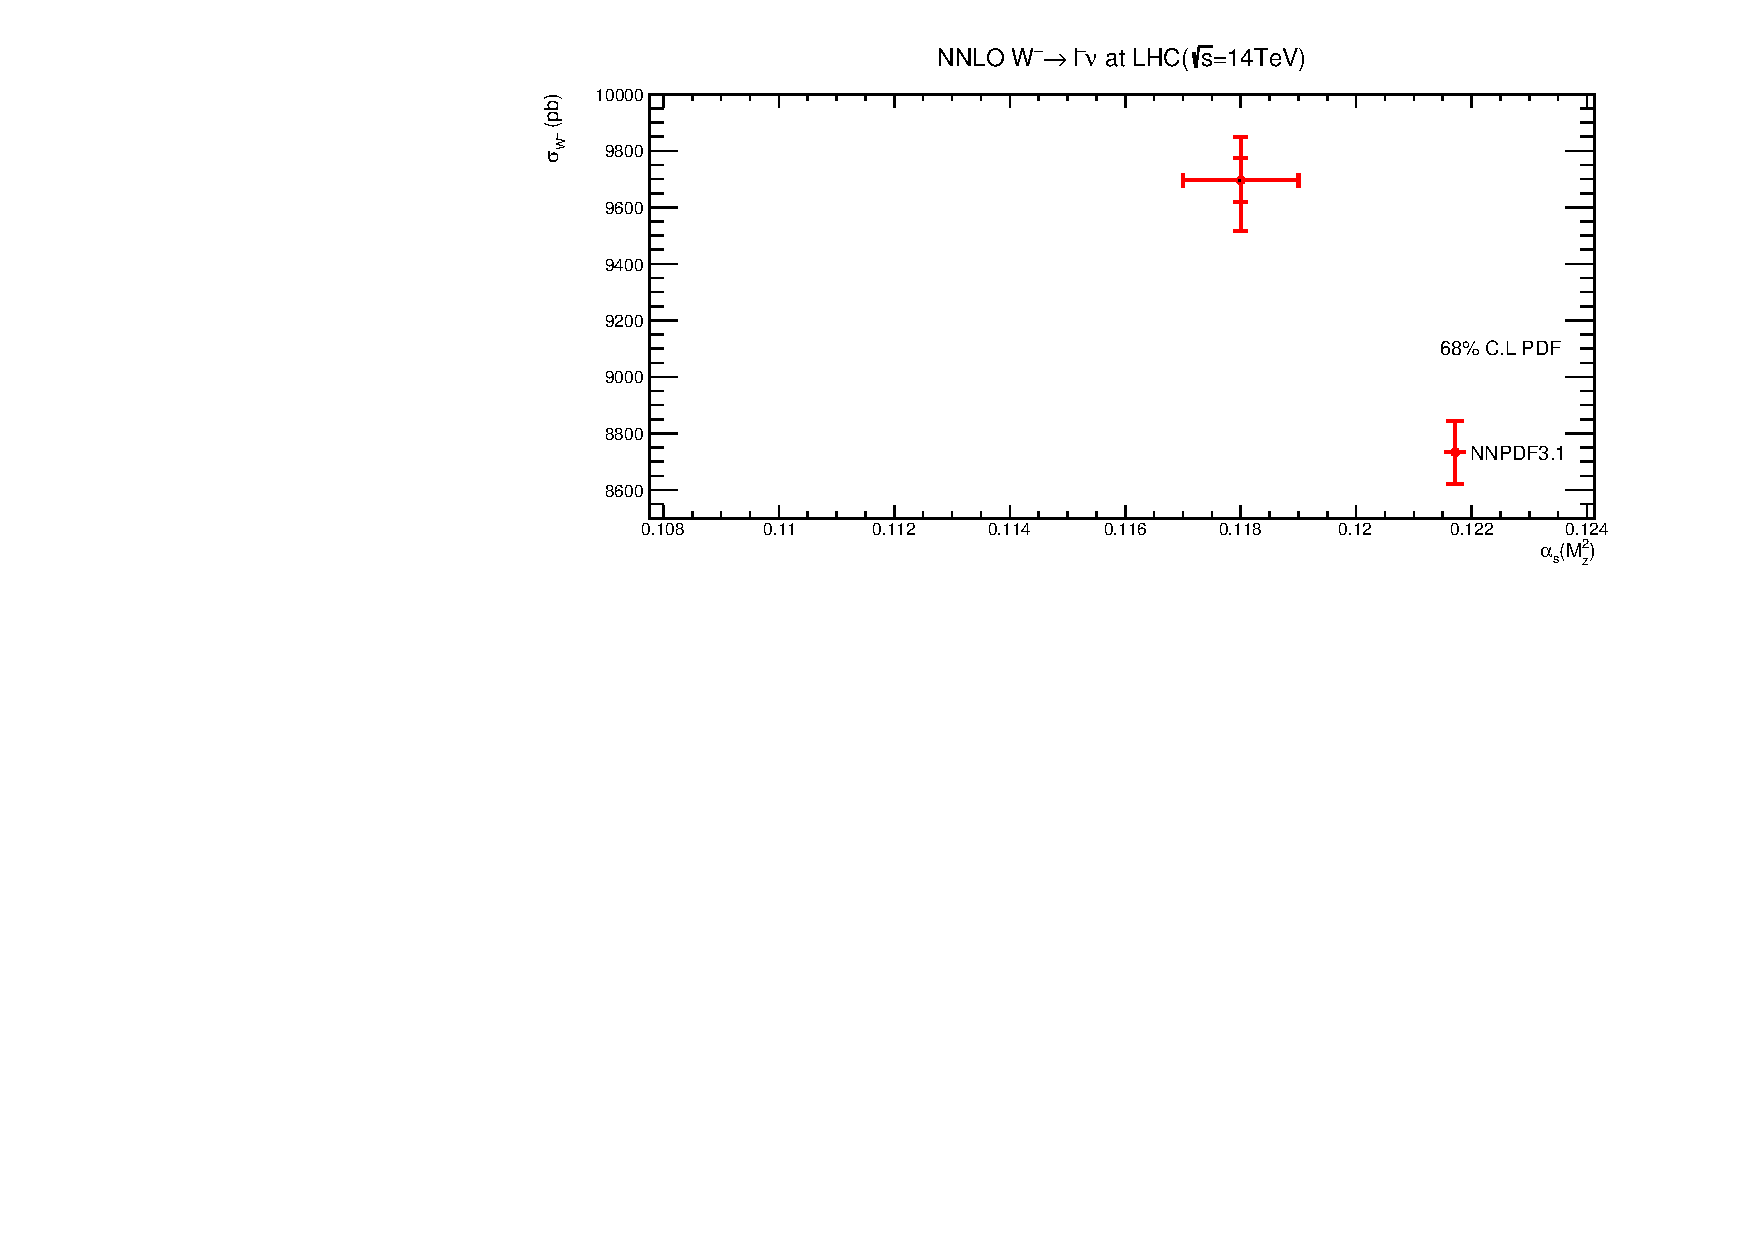
\includegraphics[height=6cm, width=\textwidth]{chapter4/Wm14.pdf}

\caption{}
\label{w-14}
\end{subfigure}
\begin{subfigure}{0.49\textwidth}
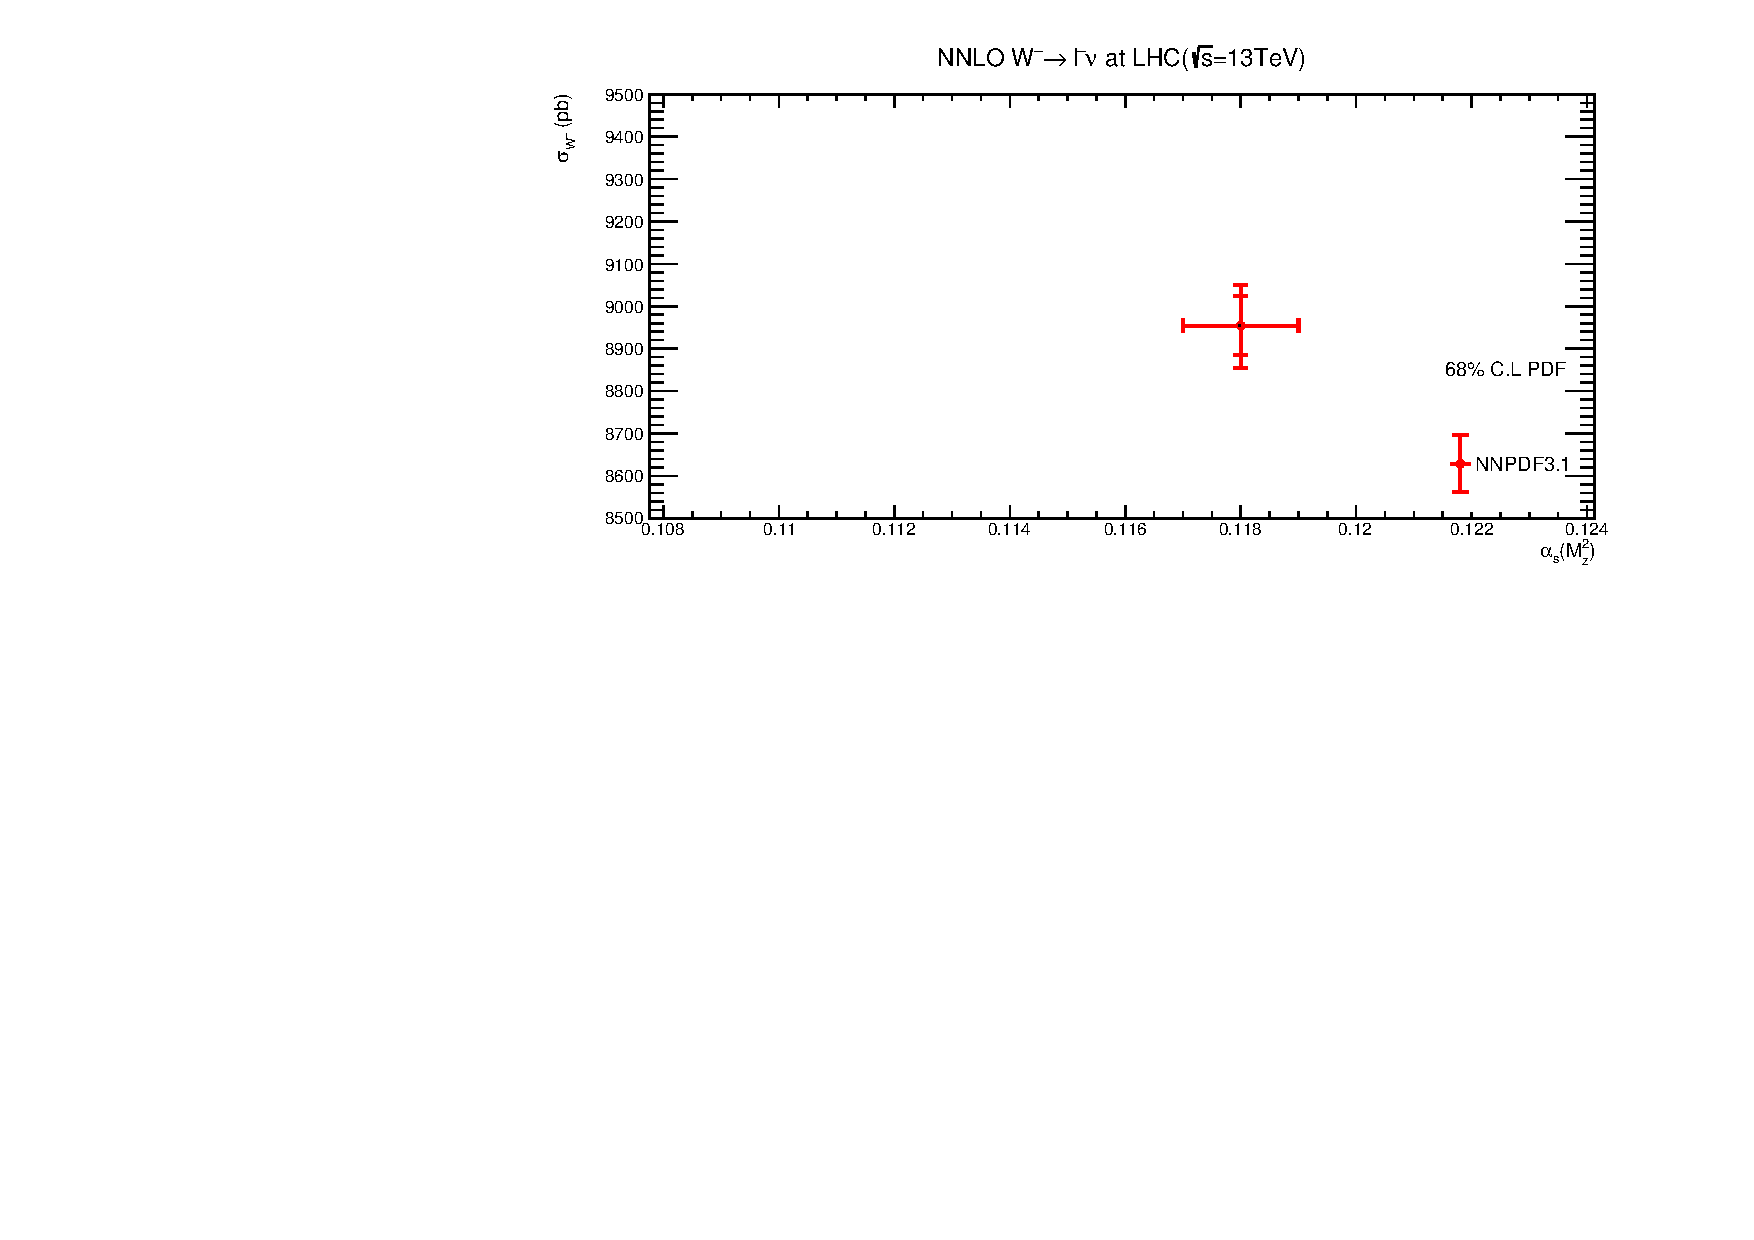
\includegraphics[height=6cm, width=\textwidth]{chapter4/Wm13.pdf}

\caption{}
\label{w-13}
\end{subfigure}
\begin{subfigure}{0.49\textwidth}
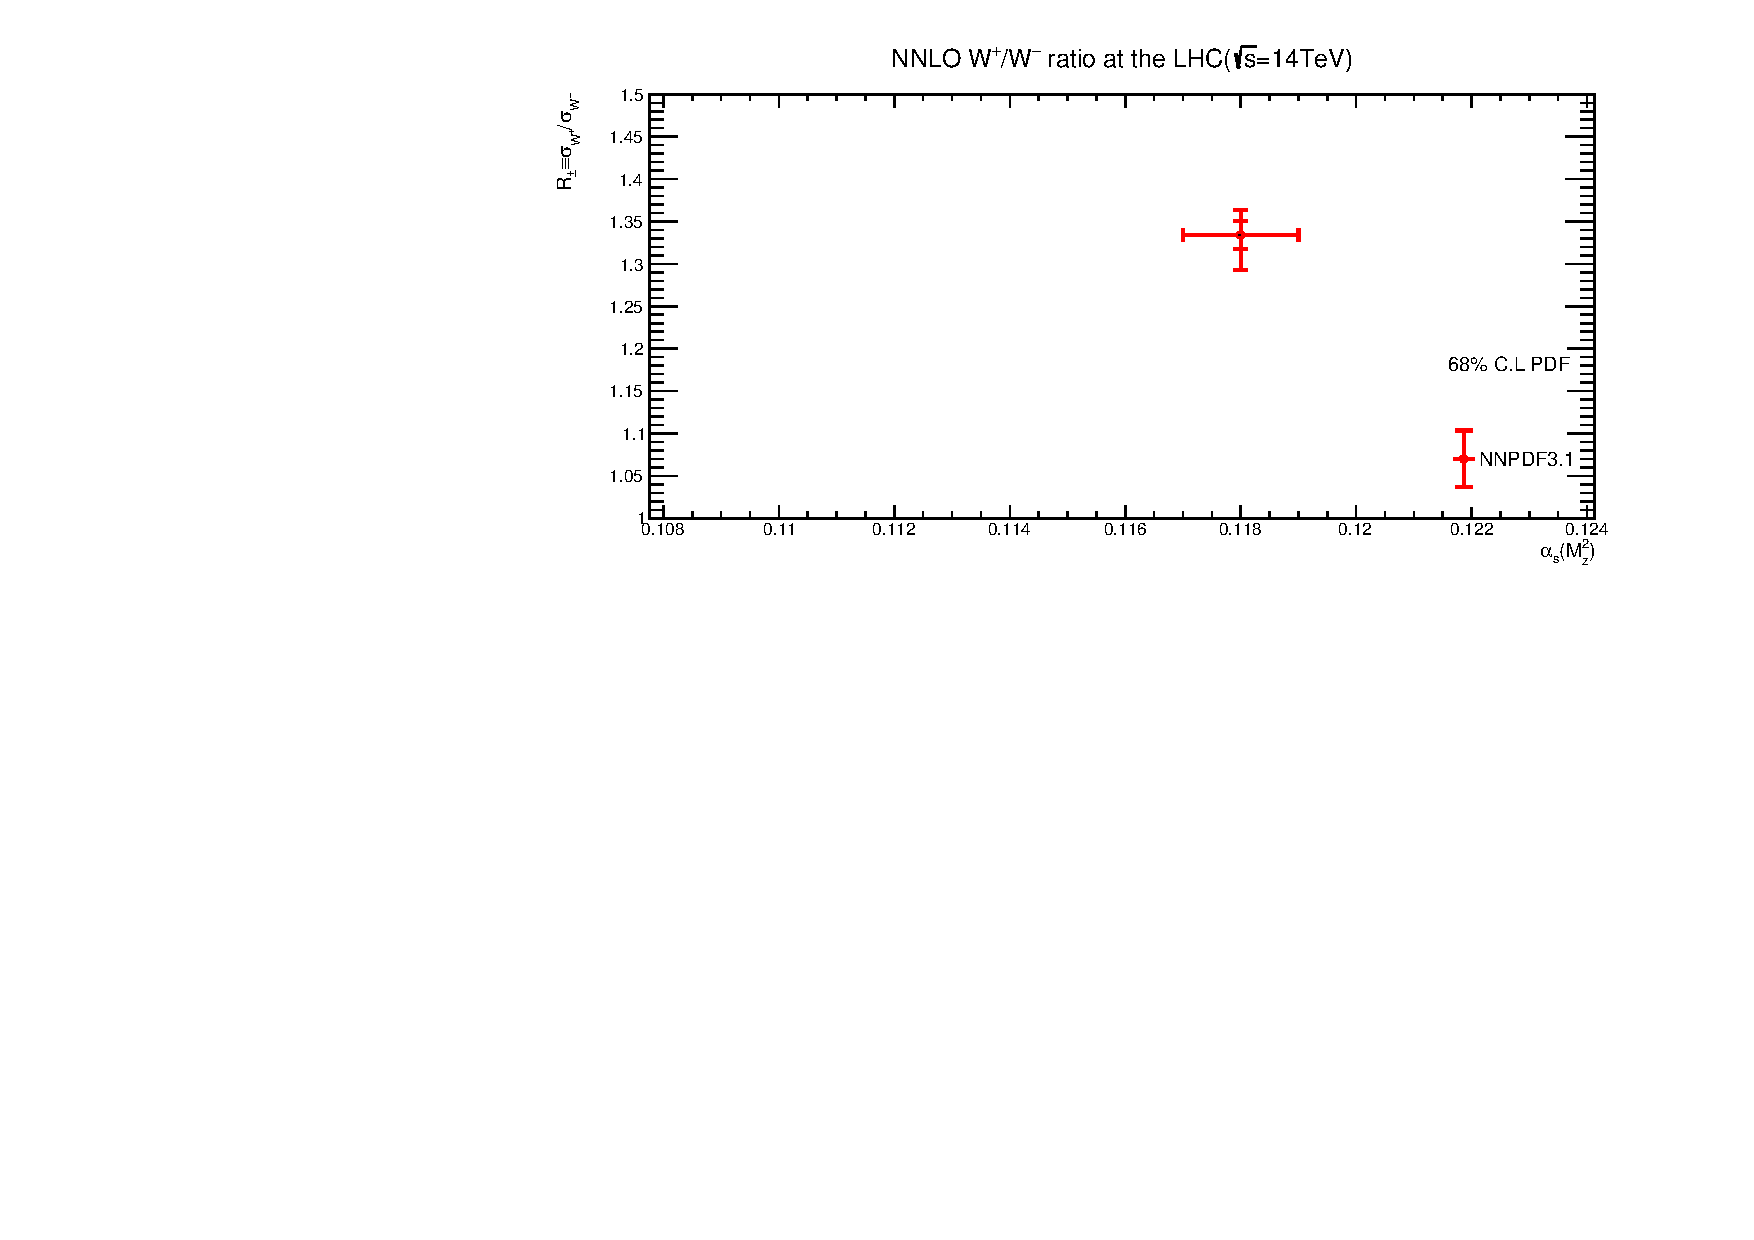
\includegraphics[height=6cm, width=\textwidth]{chapter4/Rww14.pdf}

\caption{}
\label{Rww14}
\end{subfigure}
\begin{subfigure}{0.49\textwidth}
\includegraphics[height=6cm, width=\textwidth]{chapter4/Rww13.pdf}

\caption{}
\label{Rww13}
\end{subfigure}
\caption{In Figure \ref{w+14}~\ref{w+13} are the NNLO predictions of $W^{+}$ boson production cross section at $13~TeV$ and $14~TeV$ with $68\%$ C.L. uncertainties. \ref{w-14}~\ref{w-13} are the $W^{-}$ boson production cross section and \ref{Rww14}~\ref{Rww13} are the predicted ratio of $W^{+}$ and $W^{-}$ boson production cross section at $13TeV$ and $14TeV$. The vertical error bars on prediction represent: inner~(PDF),~middle~($\alpha_{s}$),~outer~(PDF+$\alpha_{s}$~combined) error. } 
\label{13tev2}
\end{figure}

\begin{figure}[H]
\centering
\begin{subfigure}{0.49\textwidth}
\includegraphics[height=5cm ,width=\textwidth]{chapter4/W14_90.pdf}
\vspace*{-8mm}
\caption{}
\label{w14_90}
\end{subfigure}
\begin{subfigure}{0.49\textwidth}
\includegraphics[height=5cm, width=\textwidth]{chapter4/W13_90.pdf}
\vspace*{-8mm}
\caption{}
\label{w13_90}
\end{subfigure}
\begin{subfigure}{0.49\textwidth}
\includegraphics[height=5cm, width=\textwidth]{chapter4/Z14.pdf}
\vspace*{-8mm}
\caption{}
\label{z14_90}
\end{subfigure}
\begin{subfigure}{0.49\textwidth}
\includegraphics[height=5cm, width=\textwidth]{chapter4/Z13_90.pdf}
\vspace*{-8mm}
\caption{}
\label{z13_90}
\end{subfigure}
\begin{subfigure}{0.49\textwidth}
\includegraphics[height=5cm, width=\textwidth]{chapter4/Wp14_90.pdf}
\vspace*{-8mm}
\caption{}
\label{wp14_90}
\end{subfigure}
\begin{subfigure}{0.49\textwidth}
\includegraphics[height=5cm, width=\textwidth]{chapter4/Wp13_90.pdf}
\vspace*{-8mm}
\caption{}
\label{wp13_90}
\end{subfigure}
\begin{subfigure}{0.49\textwidth}
\includegraphics[height=5cm, width=\textwidth]{chapter4/Wm14_90.pdf}
\vspace*{-8mm}
\caption{}
\label{wm14_90}
\end{subfigure}
\begin{subfigure}{0.49\textwidth}
\includegraphics[height=5cm, width=\textwidth]{chapter4/Wm13_90.pdf}
\vspace*{-8mm}
\caption{}
\label{wm13_90}
\end{subfigure}
\caption{In Figure, \ref{w14_90}~\ref{w13_90} are the NNLO predictions of $W$ boson production cross section at $13~TeV$ and $14~TeV$ with $90\%$ C.L. uncertainties. \ref{z14_90}~\ref{z13_90} are the $Z$ boson production cross section and \ref{wp14_90}~\ref{wp13_90} and \ref{wm14_90}~\ref{wm13_90} showing the predicted cross section of $W^{+}$ and $W^{-}$ boson at $13~TeV$ and $14TeV$ respectively. The vertical error bars on prediction represent: inner~(PDF),~middle~($\alpha_{s}$),~outer~(PDF+$\alpha_{s}$~combined) error.} 
\label{13tev3}
\end{figure}


\begin{figure}[H]
\centering
\begin{subfigure}{0.49\textwidth}
\includegraphics[height=6cm ,width=\textwidth]{chapter4/W14_hessian.pdf}
\vspace*{-8mm}
\caption{}
\label{w14_he}
\end{subfigure}
\begin{subfigure}{0.49\textwidth}
\includegraphics[height=6cm, width=\textwidth]{chapter4/W13_hessian.pdf}
\vspace*{-8mm}
\caption{}
\label{w13_he}
\end{subfigure}
\begin{subfigure}{0.49\textwidth}
\includegraphics[height=6cm, width=\textwidth]{chapter4/Z14_hessian.pdf}
\vspace*{-8mm}
\caption{}
\label{z14_he}
\end{subfigure}
\begin{subfigure}{0.49\textwidth}
\includegraphics[height=6cm, width=\textwidth]{chapter4/Z13_hessian.pdf}
\vspace*{-8mm}
\caption{}
\label{z13_he}
\end{subfigure}
\begin{subfigure}{0.49\textwidth}
\includegraphics[height=6cm, width=\textwidth]{chapter4/Rwz_hessian.pdf}
\vspace*{-8mm}
\caption{}
\label{rwz14_he}
\end{subfigure}
\begin{subfigure}{0.49\textwidth}
\includegraphics[height=6cm, width=\textwidth]{chapter4/Rwz_hessian13.pdf}
\vspace*{-8mm}
\caption{}
\label{rwz13_he}
\end{subfigure}
\caption{In Figure, \ref{w14_he}~\ref{w13_he} are the NNLO predictions of $W^{+}$ boson production cross section at $13~TeV$ and $14~TeV$ with $90\%$ C.L. uncertainties. \ref{z14_he}~\ref{z13_he} are the $Z$ boson production cross section and \ref{rwz14_he}~\ref{rwz13_he} are the predicted ratio of $W$ and $Z$ boson production cross section at $13TeV$ and $14TeV$. These uncertainties are measured with hessian error vector method in which vertical error bars represent~inner~(PDF),~middle~($\alpha_{s}$) and~outer~(PDF+$\alpha_{s}$ combined) uncertainties.} 
\label{13tev4}
\end{figure}



\begin{figure}[H]\label{WZ13_inc}
\centering
\begin{subfigure}{0.8\textwidth}
\includegraphics[height=7cm ,width=\textwidth]{chapter4/PDF_W.pdf}
\vspace*{-8mm}
\caption{}
\label{var_cs}
\end{subfigure}
\begin{subfigure}{0.8\textwidth}
\includegraphics[height=7cm, width=\textwidth]{chapter4/PDF_Z.pdf}
\vspace*{-8mm}
\caption{}
\label{var_cs1}
\end{subfigure}
\caption{The predicted increase in production cross section of $W$ and $Z$ vector boson with the choice of $\alpha_{s}(M_{Z}^{2})$ at $13~TeV$.}
 \end{figure}

\begin{figure}[h!]{\label{w+w-_inc}}
\centering
\begin{subfigure}{0.8\textwidth}
\includegraphics[height=5.5cm, width=\textwidth]{chapter4/var_cswp_13.pdf}
\vspace*{-8mm}
\caption{}
\label{var_cs2}
\end{subfigure}
\begin{subfigure}{0.8\textwidth}
\includegraphics[height=5.5cm, width=\textwidth]{chapter4/var_cswm_13.pdf}
\vspace*{-8mm}
\caption{}
\label{var_cs3}
\end{subfigure}
\caption{The predicted increase in production cross section of $W^{+}$ ,$W^{-}$ vector boson with the choice of $\alpha_{s}(M_{Z}^{2})$ at $13~TeV$.}
 \end{figure}

\subsubsection{Variation In Cross Section With QCD Scale}
The predicted increase in cross section values of $W$ and $Z$ boson with the change in value of strong coupling constant $\alpha_{s}$ at $13~TeV$ and $14~TeV$ is shown in Fig.~\ref{var_cs}~\ref{var_cs1}~\ref{var_cs2}~\ref{var_cs3}. The variation in the predicted cross section with the change of factorization~($\mu_{F}$) and re-normalisation~($\mu_{R}$) scale simultaneously at $13~TeV$ and $14~TeV$ is shown in Fig.~\ref{comp},~\ref{comp1},~\ref{comp2} and \ref{comp3}.

\begin{figure}[H]
\centering
\begin{subfigure}{0.8\textwidth}
\includegraphics[height=7cm ,width=\textwidth]{chapter4/Comp13_68.pdf}
\vspace*{-8mm}
\caption{}
\label{rfw}
\end{subfigure}
\begin{subfigure}{0.8\textwidth}
\includegraphics[height=7cm, width=\textwidth]{chapter4/CompZ13_68.pdf}
\vspace*{-8mm}
\caption{}
\label{rfz}
\end{subfigure}
\caption{The predicted change in cross section of $W$ and $Z$ boson with the change in factorisation~$\mu_{R}$ and re-normalisation~$\mu_{F}$. \ref{rfw}~\ref{rfz} with $68\%$~C.L. at $13~TeV$ } 
\label{comp}
\end{figure}

\begin{figure}[H]
\centering
\begin{subfigure}{0.8\textwidth}
\includegraphics[height=5cm ,width=\textwidth]{chapter4/comp_wp13.pdf}
\vspace*{-8mm}
\caption{}
\label{varwp13}
\end{subfigure}
\begin{subfigure}{0.8\textwidth}
\includegraphics[height=5cm, width=\textwidth]{chapter4/comp_wm13.pdf}
\vspace*{-8mm}
\caption{}
\label{varwm13}
\end{subfigure}
\begin{subfigure}{0.8\textwidth}
\includegraphics[height=5cm, width=\textwidth]{chapter4/RwzRF_68.pdf}
\vspace*{-8mm}
\caption{}
\label{var_rat13}
\end{subfigure}
\begin{subfigure}{0.8\textwidth}
\includegraphics[height=5cm, width=\textwidth]{chapter4/RwwRF_68.pdf}
\vspace*{-8mm}
\caption{}
\label{var_rat131}
\end{subfigure}
\caption{In figure~\ref{varwp13} and\ref{varwm13} shows the predicted change in cross section of $W^{+}$ and $W^{-}$ boson with the change in factorisation~$\mu_{R}$ and re-normalisation~$\mu_{F}$ scale and~\ref{var_rat13} and~\ref{var_rat131} are the cross section ratio of $W$ to $Z$ and $W^{+}$ to $W^{-}$  boson. The vertical error bars on prediction represent: inner~(PDF),~middle~($\alpha_{s}$),~outer~(PDF+$\alpha_{s}$~combined) error.}
\label{comp1}
\end{figure}


\begin{figure}[H]
\centering
\begin{subfigure}{0.8\textwidth}
\includegraphics[height=5cm ,width=\textwidth]{chapter4/Comp14_68.pdf}
\vspace*{-8mm}
\caption{}
\label{var_14-1}
\end{subfigure}
\begin{subfigure}{0.8\textwidth}
\includegraphics[height=5cm, width=\textwidth]{chapter4/Comp14_90.pdf}
\vspace*{-8mm}
\caption{}
\label{var_14-2}
\end{subfigure}
\begin{subfigure}{0.8\textwidth}
\includegraphics[height=5cm, width=\textwidth]{chapter4/CompZ14_68.pdf}
\vspace*{-8mm}
\caption{}
\label{var_14-3}
\end{subfigure}
\begin{subfigure}{0.8\textwidth}
\includegraphics[height=5cm, width=\textwidth]{chapter4/CompZ14_90.pdf}
\vspace*{-8mm}
\caption{}
\label{var_14-4}
\end{subfigure}
\caption{The predicted change in cross section of $W$ and $Z$ boson with the change in factorisation~$\mu_{R}$ and re-normalisation~$\mu_{F}$ scale at $14~TeV$. \ref{var_14-1}~\ref{var_14-3}, with $68\%~C.L.$ and \ref{var_14-2}~\ref{var_14-4} with $90\%~C.L.$. The vertical error bars on prediction represent: inner~(PDF),~middle~($\alpha_{s}$),~outer~(PDF+$\alpha_{s}$~combined) error.}
\label{comp2} 
\end{figure}



\begin{figure}[H]
\centering
\begin{subfigure}{0.48\textwidth}
\includegraphics[height=7cm ,width=\textwidth]{chapter4/compwp14.pdf}
\vspace*{-8mm}
\caption{}
\label{wp14rf}
\end{subfigure}
\begin{subfigure}{0.49\textwidth}
\includegraphics[height=7cm, width=\textwidth]{chapter4/compwm14.pdf}
\vspace*{-8mm}
\caption{}
\label{wm14rf}
\end{subfigure}
\begin{subfigure}{0.49\textwidth}
\includegraphics[height=7cm, width=\textwidth]{chapter4/Rwz14RF_68.pdf}
\vspace*{-8mm}
\caption{}
\label{rwz14rf}
\end{subfigure}
\begin{subfigure}{0.49\textwidth}
\includegraphics[height=7cm, width=\textwidth]{chapter4/Rwz14RF_90.pdf}
\vspace*{-8mm}
\caption{}
\label{rwz14rf1}
\end{subfigure}
\begin{subfigure}{0.49\textwidth}
\includegraphics[height=7cm, width=\textwidth]{chapter4/Rww14RF_68.pdf}
\vspace*{-8mm}
\caption{}
\label{rww14rf}
\end{subfigure}
\begin{subfigure}{0.49\textwidth}
\includegraphics[height=7cm, width=\textwidth]{chapter4/Rww14RF_90.pdf}
\vspace*{-8mm}
\caption{}
\label{rww14rf1}
\end{subfigure}
\caption{In figure \ref{wp14rf}~\ref{wm14rf} showing the cross section of $W^{+}$ and $W^{-}$ boson with different QCD scales at $68\%C.L.$ uncertainties. \ref{rwz14rf}~\ref{rwz14rf1} represent the predicted change in cross section ratio of $W$ and $Z$ boson with QCD scales and \ref{rww14rf}~\ref{rww14rf1} for the $W^{+}$ and $W^{-}$ boson similarly.} 
\label{comp3}
\end{figure}


\section{Kinematics of $W$ and $Z$ Boson}
In this section generator level kinematic distributions of $W^{+}$, $W^{-}$ and $Z$ boson is presented, for LO, NLO and NNLO predictions. The kinematics are plotted at 13 and 14~TeV with QCD scale variation. The kinematics of decaying leptons from the $W\rightarrow l\nu$ and $Z\rightarrow ll$ process are also presented.
\subsection{Transverse Momentum and Pseudo Rapidity Distribution}
Figs. \ref{dist},~\ref{dist2},~\ref{dist3} and \ref{dist4} show the generator level distribution of kinematics of $W$ and $Z$ bosons at $13~TeV$ and $14~TeV$
\begin{figure}[H]
\centering
\begin{subfigure}{0.49\textwidth}
\includegraphics[height=5cm ,width=\textwidth]{chapter4/Wpt_rf1_14.pdf}
\vspace*{-8mm}
\caption{}
\label{pt141}
\end{subfigure}
\begin{subfigure}{0.49\textwidth}
\includegraphics[height=5cm, width=\textwidth]{chapter4/Wppt_rf1_13.pdf}
\vspace*{-8mm}
\caption{}
\label{pt131}
\end{subfigure}
\begin{subfigure}{0.49\textwidth}
\includegraphics[height=5cm, width=\textwidth]{chapter4/Wmpt_rf1_14.pdf}
\vspace*{-8mm}
\caption{}
\label{pt142}
\end{subfigure}
\begin{subfigure}{0.49\textwidth}
\includegraphics[height=5cm, width=\textwidth]{chapter4/Wmpt_rf1_13.pdf}
\vspace*{-8mm}
\caption{}
\label{pt132}
\end{subfigure}
\begin{subfigure}{0.49\textwidth}
\includegraphics[height=5cm, width=\textwidth]{chapter4/Zpt_rf1_14.pdf}
\vspace*{-8mm}
\caption{}
\label{pt143}
\end{subfigure}
\begin{subfigure}{0.49\textwidth}
\includegraphics[height=5cm, width=\textwidth]{chapter4/Zpt_rf1_13.pdf}
\vspace*{-8mm}
\caption{}
\label{pt133}
\end{subfigure}
\caption{In figure~\ref{pt141},~\ref{pt142},~\ref{pt143} are the theoretically predicted transverse momentum distribution of $W^{+}$, $W^{-}$ and $Z$ boson at $14~TeV$ with LO, NLO, and NNLO.\ref{pt131},~\ref{pt132},~\ref{pt133} for the $13~TeV$ for NLO and NNLO.}  
\label{dist}
\end{figure}

\begin{figure}[H]
\centering
\begin{subfigure}{0.49\textwidth}
\includegraphics[height=6cm ,width=\textwidth]{chapter4/Wpeta_rf1_14.pdf}
\vspace*{-8mm}
\caption{}
\label{eta141}
\end{subfigure}
\begin{subfigure}{0.49\textwidth}
\includegraphics[height=6cm, width=\textwidth]{chapter4/Wpeta_rf1_13.pdf}
\vspace*{-8mm}
\caption{}
\label{eta131}
\end{subfigure}
\begin{subfigure}{0.49\textwidth}
\includegraphics[height=6cm, width=\textwidth]{chapter4/Wmeta_rf1_14.pdf}
\vspace*{-8mm}
\caption{}
\label{eta142}
\end{subfigure}
\begin{subfigure}{0.49\textwidth}
\includegraphics[height=6cm, width=\textwidth]{chapter4/Wmeta_rf1_13.pdf}
\vspace*{-8mm}
\caption{}
\label{eta132}
\end{subfigure}
\begin{subfigure}{0.49\textwidth}
\includegraphics[height=6cm, width=\textwidth]{chapter4/Zeta_rf1_14.pdf}
\vspace*{-8mm}
\caption{}
\label{eta143}
\end{subfigure}
\begin{subfigure}{0.49\textwidth}
\includegraphics[height=6cm, width=\textwidth]{chapter4/Zeta_rf1_13.pdf}
\vspace*{-8mm}
\caption{}
\label{eta133}
\end{subfigure}
\caption{In figure~\ref{eta141},~\ref{eta142},~\ref{eta143} are the generator level theoretically predicted pseudo rapidity distribution of $W^{+}$, $W^{-}$ and $Z$ boson at $14~TeV$ with LO, NLO, and NNLO.\ref{eta131},~\ref{eta132},~\ref{eta133} for the $13~TeV$ for NLO and NNLO.}  
\label{dist2}
\end{figure}

\begin{figure}[H]
\centering
\begin{subfigure}{0.49\textwidth}
\includegraphics[height=6cm ,width=\textwidth]{chapter4/Wwppt_rf2_14.pdf}
\vspace*{-8mm}
\caption{}
\label{rf2pt1}
\end{subfigure}
\begin{subfigure}{0.49\textwidth}
\includegraphics[height=6cm, width=\textwidth]{chapter4/Wwpeta_rf2_14.pdf}
\vspace*{-8mm}
\caption{}
\label{rf2eta1}
\end{subfigure}
\begin{subfigure}{0.49\textwidth}
\includegraphics[height=6cm, width=\textwidth]{chapter4/Wwmpt_rf2_14.pdf}
\vspace*{-8mm}
\caption{}
\label{rf2pt2}
\end{subfigure}
\begin{subfigure}{0.49\textwidth}
\includegraphics[height=6cm, width=\textwidth]{chapter4/Wwmeta_rf2_14.pdf}
\vspace*{-8mm}
\caption{}
\label{rf2eta2}
\end{subfigure}
\begin{subfigure}{0.49\textwidth}
\includegraphics[height=6cm, width=\textwidth]{chapter4/Zpt_rf2_14.pdf}
\vspace*{-8mm}
\caption{}
\label{rf2pt3}
\end{subfigure}
\begin{subfigure}{0.49\textwidth}
\includegraphics[height=6cm, width=\textwidth]{chapter4/Zeta_rf2_14.pdf}
\vspace*{-8mm}
\caption{}
\label{rf2eta3}
\end{subfigure}
\caption{In figure~\ref{rf2pt1},~\ref{rf2pt2},~\ref{rf2pt3} are the generator level transverse momentum distribution of $W^{+}$,~$W^{-}$ and $Z$ boson at $14~TeV$ with different QCD scales.\ref{rf2eta1},~\ref{rf2eta2},~\ref{rf2eta3} are the pseudo rapidity distribution for NLO and NNLO.}  
\label{dist3}
\end{figure}

\begin{figure}[H]
\centering
\begin{subfigure}{0.49\textwidth}
\includegraphics[height=6cm ,width=\textwidth]{chapter4/WpY14.pdf}
\vspace*{-8mm}
\caption{}
\label{wpy14}
\end{subfigure}
\begin{subfigure}{0.49\textwidth}
\includegraphics[height=6cm, width=\textwidth]{chapter4/WpY13.pdf}
\vspace*{-8mm}
\caption{}
\label{wpy13}
\end{subfigure}
\begin{subfigure}{0.49\textwidth}
\includegraphics[height=6cm, width=\textwidth]{chapter4/WmY14.pdf}
\vspace*{-8mm}
\caption{}
\label{wmy14}
\end{subfigure}
\begin{subfigure}{0.49\textwidth}
\includegraphics[height=6cm, width=\textwidth]{chapter4/WmY13.pdf}
\vspace*{-8mm}
\caption{}
\label{wmy13}
\end{subfigure}
\begin{subfigure}{0.49\textwidth}
\includegraphics[height=6cm, width=\textwidth]{chapter4/ZY14.pdf}
\vspace*{-8mm}
\caption{}
\label{zy14}
\end{subfigure}
\begin{subfigure}{0.49\textwidth}
\includegraphics[height=6cm, width=\textwidth]{chapter4/ZY13.pdf}
\vspace*{-8mm}
\caption{}
\label{zy13}
\end{subfigure}
\caption{In figure~\ref{wpy14},~\ref{wpy13}~are the generator level rapidity distribution of $W^{+}$ boson at $14~TeV$ and $13~TeV$.\ref{wmy14},~\ref{wmy13}~for the  $W^{-}$ boson and \ref{zy14}~\ref{zy13}for $Z$ boson rapidity distribution.}  
\label{dist4}
\end{figure}


\section{Leptons $p_{T}$ and $\eta$ Distribution}
Figs. \ref{elec} and \ref{elec1} show the electron $p_{T}$ and $\eta$ distribution at $13~TeV$ and $14~TeV$.
\begin{figure}[H]
\centering
\begin{subfigure}{0.49\textwidth}
\includegraphics[height=6cm ,width=\textwidth]{chapter4/Ewppt_rf1_14.pdf}
\vspace*{-8mm}
\caption{}
\label{ept141}
\end{subfigure}
\begin{subfigure}{0.49\textwidth}
\includegraphics[height=6cm, width=\textwidth]{chapter4/Ewppt_rf1_13.pdf}
\vspace*{-8mm}
\caption{}
\label{ept131}
\end{subfigure}
\begin{subfigure}{0.49\textwidth}
\includegraphics[height=6cm, width=\textwidth]{chapter4/Ewmpt_rf1_14.pdf}
\vspace*{-8mm}
\caption{}
\label{ept142}
\end{subfigure}
\begin{subfigure}{0.49\textwidth}
\includegraphics[height=6cm, width=\textwidth]{chapter4/Ewmpt_rf1_13.pdf}
\vspace*{-8mm}
\caption{}
\label{ept132}
\end{subfigure}
\begin{subfigure}{0.49\textwidth}
\includegraphics[height=6cm, width=\textwidth]{chapter4/Ezpt_rf1_14.pdf}
\vspace*{-8mm}
\caption{}
\label{ept143}
\end{subfigure}
\begin{subfigure}{0.49\textwidth}
\includegraphics[height=6cm, width=\textwidth]{chapter4/Ezpt_rf1_13.pdf}
\vspace*{-8mm}
\caption{}
\label{ept133}
\end{subfigure}
\caption{In figure~\ref{ept141},~\ref{ept142},~\ref{ept143} are the generator level transverse momentum distribution of electron at $14~TeV$ with LO, NLO, and NNLO.\ref{ept131},~\ref{ept132},~\ref{ept133} for the $13~TeV$ for NLO and NNLO.}  
\label{elec}
\end{figure}




\begin{figure}[H]
\centering
\begin{subfigure}{0.49\textwidth}
\includegraphics[height=6cm ,width=\textwidth]{chapter4/Ewpeta_rf1_14.pdf}
\vspace*{-8mm}
\caption{}
\label{eeta141}
\end{subfigure}
\begin{subfigure}{0.49\textwidth}
\includegraphics[height=6cm, width=\textwidth]{chapter4/Ewpeta_rf1_13.pdf}
\vspace*{-8mm}
\caption{}
\label{eeta131}
\end{subfigure}
\begin{subfigure}{0.49\textwidth}
\includegraphics[height=6cm, width=\textwidth]{chapter4/Ewmeta_rf1_14.pdf}
\vspace*{-8mm}
\caption{}
\label{eeta142}
\end{subfigure}
\begin{subfigure}{0.49\textwidth}
\includegraphics[height=6cm, width=\textwidth]{chapter4/Ewmeta_rf1_13.pdf}
\vspace*{-8mm}
\caption{}
\label{eeta132}
\end{subfigure}
\begin{subfigure}{0.49\textwidth}
\includegraphics[height=6cm, width=\textwidth]{chapter4/Ezeta_rf1_14.pdf}
\vspace*{-8mm}
\caption{}
\label{eeta143}
\end{subfigure}
\begin{subfigure}{0.49\textwidth}
\includegraphics[height=6cm, width=\textwidth]{chapter4/Ezeta_rf1_13.pdf}
\vspace*{-8mm}
\caption{}
\label{eeta133}
\end{subfigure}
\caption{In figure~\ref{eeta141},~\ref{eeta142},~\ref{eeta143} are the generator level pseudo rapidity distribution of electron at $14~TeV$ with LO, NLO, and NNLO.\ref{eeta131},~\ref{eeta132},~\ref{eeta133} for the $13~TeV$ for NLO and NNLO.}  
\label{elec1}
\end{figure}






\subsection{Di-lepton Mass and Rapidity Distribution}
The plots in Figs.~\ref{dilep} and \ref{delep1} show the distribution of rapidity and Di-lepton mass from $W\rightarrow e\nu$, $Z\rightarrow ll$ events at the generator level.
\begin{figure}[H]
\centering
\begin{subfigure}{0.49\textwidth}
\includegraphics[height=6cm ,width=\textwidth]{chapter4/WpYE14.pdf}
\vspace*{-8mm}
\caption{}
\label{wpey14}
\end{subfigure}
\begin{subfigure}{0.49\textwidth}
\includegraphics[height=6cm, width=\textwidth]{chapter4/WpYE13.pdf}
\vspace*{-8mm}
\caption{}
\label{wpey13}
\end{subfigure}
\begin{subfigure}{0.49\textwidth}
\includegraphics[height=6cm, width=\textwidth]{chapter4/WmYE14.pdf}
\vspace*{-8mm}
\caption{}
\label{wmey14}
\end{subfigure}
\begin{subfigure}{0.49\textwidth}
\includegraphics[height=6cm, width=\textwidth]{chapter4/WmYE13.pdf}
\vspace*{-8mm}
\caption{}
\label{wmey13}
\end{subfigure}
\begin{subfigure}{0.49\textwidth}
\includegraphics[height=6cm, width=\textwidth]{chapter4/ZEY14.pdf}
\vspace*{-8mm}
\caption{}
\label{zey14}
\end{subfigure}
\begin{subfigure}{0.49\textwidth}
\includegraphics[height=6cm, width=\textwidth]{chapter4/ZEY13.pdf}
\vspace*{-8mm}
\caption{}
\label{zey13}
\end{subfigure}
\caption{In figure~\ref{wpey14},~\ref{wpey13}~are the generator level rapidity distribution of electron for $W^{+}$ boson event at $14~TeV$~and~$13TeV$, \ref{wmey14},~\ref{wmey13} for $W^{-}$ and ~\ref{zey14},~\ref{zey13} for the $Z$ boson event.}  
\label{dilep}
\end{figure}


\begin{figure}[H]
\centering
\begin{subfigure}{0.49\textwidth}
\includegraphics[height=6cm ,width=\textwidth]{chapter4/Mll_rf1_14.pdf}
\vspace*{-8mm}
\caption{}
\label{mll14}
\end{subfigure}
\begin{subfigure}{0.49\textwidth}
\includegraphics[height=6cm, width=\textwidth]{chapter4/Mll_rf1_13.pdf}
\vspace*{-8mm}
\caption{}
\label{mll13}
\end{subfigure}
\begin{subfigure}{0.49\textwidth}
\includegraphics[height=6cm, width=\textwidth]{chapter4/Mll_rf2_14.pdf}
\vspace*{-8mm}
\caption{}
\label{mll142}
\end{subfigure}
\begin{subfigure}{0.49\textwidth}
\includegraphics[height=6cm, width=\textwidth]{chapter4/Mll_rf0.5_14.pdf}
\vspace*{-8mm}
\caption{}
\label{mll140}
\end{subfigure}

\caption{In figure~\ref{mll14},~\ref{mll142},~\ref{mll140} are the generator level Di-lepton transverse momentum distribution at $14~TeV$ with different QCD scales.} 
\label{delep1} 
\end{figure}


\chapter*{Conclusion}
The study of single vector boson production cross section is very important because these bosons form background events for many important processes in Standard Model, specially events involving Higgs boson and Top quark. The precise measurement of vector boson gives deep insight to understand quantum chromodynamics~(QCD) and electroweak~(EW) processes.\\
We performed a detail study of $W$ and $Z$ vector boson production cross section~i.e.~$\sigma\times BR(W\rightarrow l\nu, Z\rightarrow ll)$. The measured results of vector boson production cross section at $7~TeV\approx~ 40pb^{-1}$, $8~TeV\approx 18.2~pb^{-1}$ and $13~TeV\approx 81~pb^{-1}$ are compared with the theoretically predicted cross sections.We find a great agreement between measured and theoretically predicted cross sections.\\
We also studied about various theoretical uncertainties in the predictions including PDF, $\alpha_{s}$, QCD scale uncertainties etc. We also find how the $W$ and $Z$ boson cross section ratios are beneficial in cancellation of certain experimental and theoretical uncertainties.\\
The Predicted kinematics of these vector bosons and corresponding leptons are measured in detail and compared with the measured results.\\
We also made theoretical prediction for vector boson production cross section at $14~TeV$ at various QCD scales. These prediction will be checked with the measurements when the data will be available. We hope that these predictions at $14~TeV$ will be comparable with the measurements as were the previous results.





